\chapter{已知赛道环境中基于控制障碍函数的安全运动控制}
基于模型的运动控制方法在自动驾驶领域已经相对成熟，然而对于高速运动的赛车，如何在保证安全的前提下实现高性能控制仍然是一个具有挑战性的问题。本章针对已知赛道环境中的自动驾驶赛车控制问题，提出了一种基于控制障碍函数的安全运动控制方法。首先，我们建立了车辆的动力学模型，并通过参数辨识方法获取了模型中的关键参数。随后，我们介绍了控制障碍函数的基本概念，并设计了一种基于控制障碍函数的模型预测控制策略，以确保赛车在竞速过程中能够安全地避开障碍物和赛道边界。最后，我们通过仿真和实车实验验证了所提方法的有效性和实用性。
\section{动力学建模与参数辨识}
本节首先介绍了赛车的动力学模型，包括车辆的运动学方程和动力学方程。随后，我们采用实验数据对模型中的关键参数进行了辨识，以确保模型能够准确地描述赛车的运动行为。这些参数包括车辆的质量、轮胎的摩擦系数、轮胎侧偏刚度等。通过参数辨识，我们为后续的控制设计提供了可靠的模型基础。
\subsection{车辆动力学模型}
本文的赛车平台是一个1：10比例的阿克曼底盘赛车，具有前轮转向和后轮驱动的结构。为了描述赛车的运动行为，我们采用了一个基于单轨模型的动力学模型\cite{rajamani2006vehicle}，如图\ref{fig:car-model}所示。单轨模型（又称为自行车模型）是一种简化的车辆动力学模型，能够有效描述车辆的横向和纵向运动特性。其核心思想是将车辆的四个轮子简化为一个前轮和一个后轮，在保留车辆的主要动力学特性的同时降低模型的复杂度。模型做出了以下假设：车辆左右轮胎动力学对称，车辆仅考虑在平面内运动，轮胎力集中于轴中心，且忽略了车辆的悬挂系统和车身的滚转、俯仰等动态效应。
\begin{figure}[ht]
    \centering
    

\tikzset{every picture/.style={line width=0.75pt}} %set default line width to 0.75pt

\begin{tikzpicture}[x=0.75pt,y=0.75pt,yscale=-1,xscale=1]
%uncomment if require: \path (0,273); %set diagram left start at 0, and has height of 273

%Straight Lines [id:da7719784620419559]
\draw [line width=1.5]    (265.45,156.24) -- (381.67,97.67) ;
%Rounded Rect [id:dp09589244337872227]
\draw  [line width=0.75]  (365.34,115.38) .. controls (363.62,114.46) and (363.02,112.36) .. (363.99,110.67) -- (383.79,76.39) .. controls (384.76,74.7) and (386.94,74.08) .. (388.66,74.99) -- (397.99,79.96) .. controls (399.71,80.87) and (400.31,82.97) .. (399.34,84.66) -- (379.55,118.94) .. controls (378.57,120.63) and (376.39,121.25) .. (374.67,120.34) -- cycle ;
%Straight Lines [id:da9107485053132169]
\draw  [dash pattern={on 4.5pt off 4.5pt}]  (381.67,97.67) -- (431.89,71) ;
%Straight Lines [id:da7236581188251998]
\draw [color={rgb, 255:red, 245; green, 166; blue, 35 }  ,draw opacity=1 ][line width=1.5]    (252.24,162.81) -- (295.09,141.45) ;
\draw [shift={(298.67,139.67)}, rotate = 153.51] [fill={rgb, 255:red, 245; green, 166; blue, 35 }  ,fill opacity=1 ][line width=0.08]  [draw opacity=0] (15.6,-3.9) -- (0,0) -- (15.6,3.9) -- cycle    ;
%Straight Lines [id:da2345090417358633]
\draw [color={rgb, 255:red, 245; green, 166; blue, 35 }  ,draw opacity=1 ][line width=1.5]    (252.24,162.81) -- (231.56,124.19) ;
\draw [shift={(229.67,120.67)}, rotate = 61.83] [fill={rgb, 255:red, 245; green, 166; blue, 35 }  ,fill opacity=1 ][line width=0.08]  [draw opacity=0] (15.6,-3.9) -- (0,0) -- (15.6,3.9) -- cycle    ;
%Straight Lines [id:da13192673239394748]
\draw  [dash pattern={on 4.5pt off 4.5pt}]  (252.24,162.81) -- (278.24,213.81) ;
%Straight Lines [id:da7431772516827679]
\draw  [dash pattern={on 4.5pt off 4.5pt}]  (381.67,97.67) -- (407.67,148.67) ;
%Straight Lines [id:da09341401254024317]
\draw [color={rgb, 255:red, 126; green, 211; blue, 33 }  ,draw opacity=1 ][line width=1.5]    (317.24,129.81) -- (355.31,110.79) ;
\draw [shift={(358.89,109)}, rotate = 153.45] [fill={rgb, 255:red, 126; green, 211; blue, 33 }  ,fill opacity=1 ][line width=0.08]  [draw opacity=0] (15.6,-3.9) -- (0,0) -- (15.6,3.9) -- cycle    ;
%Straight Lines [id:da930566701836]
\draw [color={rgb, 255:red, 126; green, 211; blue, 33 }  ,draw opacity=1 ][line width=1.5]    (317.24,129.81) -- (296.56,91.19) ;
\draw [shift={(294.67,87.67)}, rotate = 61.83] [fill={rgb, 255:red, 126; green, 211; blue, 33 }  ,fill opacity=1 ][line width=0.08]  [draw opacity=0] (15.6,-3.9) -- (0,0) -- (15.6,3.9) -- cycle    ;
%Straight Lines [id:da2713517829094356]
\draw  [dash pattern={on 4.5pt off 4.5pt}]  (317.24,129.81) -- (343.24,180.81) ;
%Straight Lines [id:da4899430101257738]
\draw [line width=0.75]    (273.74,206.81) -- (404.74,142.81) ;
%Straight Lines [id:da39204459222601296]
\draw    (271.81,200.95) -- (278.24,213.81) ;
%Straight Lines [id:da9324309786355234]
\draw    (336.81,167.95) -- (343.24,180.81) ;
%Straight Lines [id:da34772620532399245]
\draw    (401.24,135.81) -- (407.67,148.67) ;
%Straight Lines [id:da3864334623108914]
\draw  [dash pattern={on 4.5pt off 4.5pt}]  (381.67,97.67) -- (411.89,45) ;
%Shape: Arc [id:dp7662248610550513]
\draw  [draw opacity=0][line width=1.5]  (326.36,139.39) .. controls (323.96,141.52) and (320.75,142.81) .. (317.24,142.81) .. controls (309.78,142.81) and (303.74,136.99) .. (303.74,129.81) .. controls (303.74,123.22) and (308.82,117.78) .. (315.42,116.93) -- (317.24,129.81) -- cycle ; \draw  [color={rgb, 255:red, 74; green, 144; blue, 226 }  ,draw opacity=1 ][line width=1.5]  (326.36,139.39) .. controls (323.96,141.52) and (320.75,142.81) .. (317.24,142.81) .. controls (309.78,142.81) and (303.74,136.99) .. (303.74,129.81) .. controls (303.74,123.22) and (308.82,117.78) .. (315.42,116.93) ;
%Shape: Triangle [id:dp8756825061990094]
\draw  [color={rgb, 255:red, 74; green, 144; blue, 226 }  ,draw opacity=1 ][fill={rgb, 255:red, 74; green, 144; blue, 226 }  ,fill opacity=1 ] (330.67,129.41) -- (329.79,140) -- (324.77,138.17) -- cycle ;
%Straight Lines [id:da09074034690483157]
\draw [color={rgb, 255:red, 245; green, 166; blue, 35 }  ,draw opacity=1 ][line width=1.5]    (381.67,97.67) -- (342.37,75.13) ;
\draw [shift={(338.9,73.14)}, rotate = 29.83] [fill={rgb, 255:red, 245; green, 166; blue, 35 }  ,fill opacity=1 ][line width=0.08]  [draw opacity=0] (15.6,-3.9) -- (0,0) -- (15.6,3.9) -- cycle    ;
%Straight Lines [id:da6145637530172485]
\draw  [dash pattern={on 4.5pt off 4.5pt}]  (381.67,97.67) -- (384.89,40) ;
%Shape: Arc [id:dp5179753373168106]
\draw  [draw opacity=0][line width=1.5]  (384.45,62.64) .. controls (385.78,62.22) and (387.19,61.99) .. (388.66,61.99) .. controls (393.29,61.99) and (397.38,64.24) .. (399.81,67.67) -- (388.66,74.99) -- cycle ; \draw  [color={rgb, 255:red, 74; green, 144; blue, 226 }  ,draw opacity=1 ][line width=1.5]  (384.45,62.64) .. controls (385.78,62.22) and (387.19,61.99) .. (388.66,61.99) .. controls (393.29,61.99) and (397.38,64.24) .. (399.81,67.67) ;
%Shape: Arc [id:dp44228022218032126]
\draw  [draw opacity=0][line width=1.5]  (399.81,67.67) .. controls (400.01,67.66) and (400.22,67.65) .. (400.43,67.65) .. controls (407.88,67.65) and (413.93,73.47) .. (413.93,80.65) .. controls (413.93,80.77) and (413.93,80.88) .. (413.92,81) -- (400.43,80.65) -- cycle ; \draw  [color={rgb, 255:red, 126; green, 211; blue, 33 }  ,draw opacity=1 ][line width=1.5]  (399.81,67.67) .. controls (400.01,67.66) and (400.22,67.65) .. (400.43,67.65) .. controls (407.88,67.65) and (413.93,73.47) .. (413.93,80.65) .. controls (413.93,80.77) and (413.93,80.88) .. (413.92,81) ;
%Straight Lines [id:da07400618834280537]
\draw  [dash pattern={on 4.5pt off 4.5pt}]  (317.24,129.81) -- (364.89,129) ;
%Shape: Arc [id:dp2521543667068522]
\draw  [draw opacity=0][line width=1.5]  (340.05,118.8) .. controls (342.11,121.09) and (343.36,124.07) .. (343.36,127.33) .. controls (343.36,128.02) and (343.31,128.69) .. (343.2,129.34) -- (329.86,127.33) -- cycle ; \draw  [color={rgb, 255:red, 245; green, 166; blue, 35 }  ,draw opacity=1 ][line width=1.5]  (340.05,118.8) .. controls (342.11,121.09) and (343.36,124.07) .. (343.36,127.33) .. controls (343.36,128.02) and (343.31,128.69) .. (343.2,129.34) ;
%Rounded Rect [id:dp31997282329303633]
\draw  [line width=0.75]  (228.8,168.36) .. controls (227.89,166.65) and (228.56,164.56) .. (230.31,163.71) -- (265.89,146.35) .. controls (267.64,145.5) and (269.8,146.2) .. (270.71,147.92) -- (275.68,157.25) .. controls (276.59,158.97) and (275.91,161.06) .. (274.16,161.91) -- (238.58,179.26) .. controls (236.83,180.12) and (234.68,179.41) .. (233.76,177.7) -- cycle ;
%Straight Lines [id:da08889167466547088]
\draw  [dash pattern={on 4.5pt off 4.5pt}]  (252.24,162.81) -- (272.89,109) ;
%Shape: Arc [id:dp2783789579468383]
\draw  [draw opacity=0][line width=1.5]  (259.85,140.5) .. controls (260.59,140.38) and (261.35,140.31) .. (262.12,140.31) .. controls (268.85,140.31) and (274.42,145.04) .. (275.45,151.24) -- (262.12,153.31) -- cycle ; \draw  [color={rgb, 255:red, 126; green, 211; blue, 33 }  ,draw opacity=1 ][line width=1.5]  (259.85,140.5) .. controls (260.59,140.38) and (261.35,140.31) .. (262.12,140.31) .. controls (268.85,140.31) and (274.42,145.04) .. (275.45,151.24) ;

% Text Node
\draw (308,193.73) node [anchor=north west][inner sep=0.75pt]    {$l_{r}$};
% Text Node
\draw (375,160.4) node [anchor=north west][inner sep=0.75pt]    {$l_{f}$};
% Text Node
\draw (206,122.4) node [anchor=north west][inner sep=0.75pt]    {$F_{y,r}$};
% Text Node
\draw (277.45,154.64) node [anchor=north west][inner sep=0.75pt]    {$F_{x}$};
% Text Node
\draw (342,51.4) node [anchor=north west][inner sep=0.75pt]    {$F_{y,f}$};
% Text Node
\draw (386.9,35.54) node [anchor=north west][inner sep=0.75pt]    {$\alpha _{f}$};
% Text Node
\draw (414,54.4) node [anchor=north west][inner sep=0.75pt]    {$\delta $};
% Text Node
\draw (329,94.4) node [anchor=north west][inner sep=0.75pt]    {$v_{x}$};
% Text Node
\draw (301,76.4) node [anchor=north west][inner sep=0.75pt]    {$v_{y}$};
% Text Node
\draw (308,145.4) node [anchor=north west][inner sep=0.75pt]    {$\omega $};
% Text Node
\draw (347,114.4) node [anchor=north west][inner sep=0.75pt]    {$\theta $};
% Text Node
\draw (271.9,124.54) node [anchor=north west][inner sep=0.75pt]    {$\alpha _{r}$};


\end{tikzpicture}

    \caption{车辆动力学模型}
    \label{fig:car-model}
\end{figure}

该模型的状态变量为$\boldsymbol{x}=[X,Y,\phi, v_x,v_y,\omega]^\top$，其中$X$和$Y$表示车辆质心在全局坐标系下的位置，$\phi$表示车辆的航向角，$v_x$和$v_y$分别表示车辆在车身坐标系下的纵向和横向速度，$\omega$表示车辆的偏航角速度。控制输入为$\boldsymbol{u}=[\delta, T]^\top$，其中$\delta$表示前轮转角，$T$表示后轮驱动输入，$T=1$表示全油门，$T=-1$表示全刹车。车辆的动力学方程可以表示为：
\begin{equation}
\begin{aligned}
    \dot{v_x}&=\frac{1}{m}(F_x-F_{y,f}\sin{\delta}+mv_y\omega),\\
    \dot{v_y}&=\frac{1}{m}(F_{y,r}+F_{y,f}\cos{\delta}-mv_x\omega),\\
    \dot{\omega}&=\frac{1}{I_z}(F_{y,f}l_f\cos{\delta}-F_{y,r}l_r),
\end{aligned}
\label{equ:car-dynamics}
\end{equation}
其中$m$表示车辆的质量，$I_z$表示车辆的偏航转动惯量，$l_f$和$l_r$分别表示前轴和后轴到车辆质心的距离，$F_x$表示车辆的纵向驱动力，$F_{y,f}$和$F_{y,r}$分别表示前轮和后轮的横向力。由车辆的运动学关系，我们还可以推出车辆的运动学方程：
\begin{equation}
\begin{aligned}
    \dot{X}&=v_x\cos{\phi}-v_y\sin{\phi},\\
    \dot{Y}&=v_x\sin{\phi}+v_y\cos{\phi},\\
    \dot{\phi}&=\omega.
\end{aligned}
\end{equation}

为了完整描述车辆的动力学行为，我们还需要建立轮胎模型来计算轮胎力。本文采用了基于魔术公式（Magic Formula，简称MF）的轮胎模型\cite{pacejka2005tire}，该模型能够准确地描述轮胎在不同工况下的力学特性。魔术公式模型的核心思想是通过一系列参数化的函数来描述轮胎的纵向和横向力与轮胎侧偏角之间的关系。下面首先推导侧偏角的计算方法，然后介绍魔术公式模型的具体形式。

侧偏角$\alpha_{f/r}$是描述轮胎横向滑移程度的一个重要参数，定义为轮胎的横向速度与纵向速度之比。车辆可被视为一个刚体，刚体上任意一点的速度$\vec{v}_P$可由质心CG的速度$\vec{v}_{CG}$和角速度$\vec{\omega}$以及P到CG的距离$\vec{r}_{P,CG}$计算：
\begin{equation}
\begin{aligned}
    \vec{v}_P=\vec{v}_{CG}+\vec{\omega}\times \vec{r}_{P,CG}.
\end{aligned}
\end{equation}
因此，对于前轮和后轮，侧偏角的计算方法如下：
\begin{equation}
\begin{aligned}
    \alpha_{f}&=-\arctan{\left(\frac{v_y+l_f\omega}{v_x}\right)}+\delta,\\
    \alpha_{r}&=\arctan{\left(\frac{l_r\omega-v_y}{v_x}\right)}.
\end{aligned}
\label{equ:slip-angle}
\end{equation}

魔术公式模型通过一系列参数化的函数来描述轮胎的纵向和横向力与轮胎侧偏角之间的关系。对于横向力，魔术公式模型的表达式如下：
\begin{equation}
\begin{aligned}
    F_{y}(\alpha)=D\sin{(C\arctan{(B\alpha-E(B\alpha-\arctan{B\alpha}))})},
\end{aligned}
\end{equation}
其中$B$、$C$、$D$和$E$是魔术公式模型的参数。$B$控制轮胎力与侧偏角的刚度；$C$控制轮胎力的形状，$BCD$控制摩擦力在线性区的斜率；$D$控制轮胎力的幅值，一般来说$D=\mu F_z$，其中$\mu$为轮胎与地面的摩擦系数，$F_z$为轮胎的垂向载荷；$E$控制饱和后轮胎力的曲线偏移。通过调整这些参数，魔术公式模型能够适应不同类型的轮胎和不同的路面条件，从而准确地描述轮胎的力学特性。图\ref{fig:magic-formula}展示了一个魔术公式曲线的示例，其中参数设置为$B=10$，$C=1.5$，$D=15$，$E=0.1$。
\begin{figure}[ht]
    \centering
    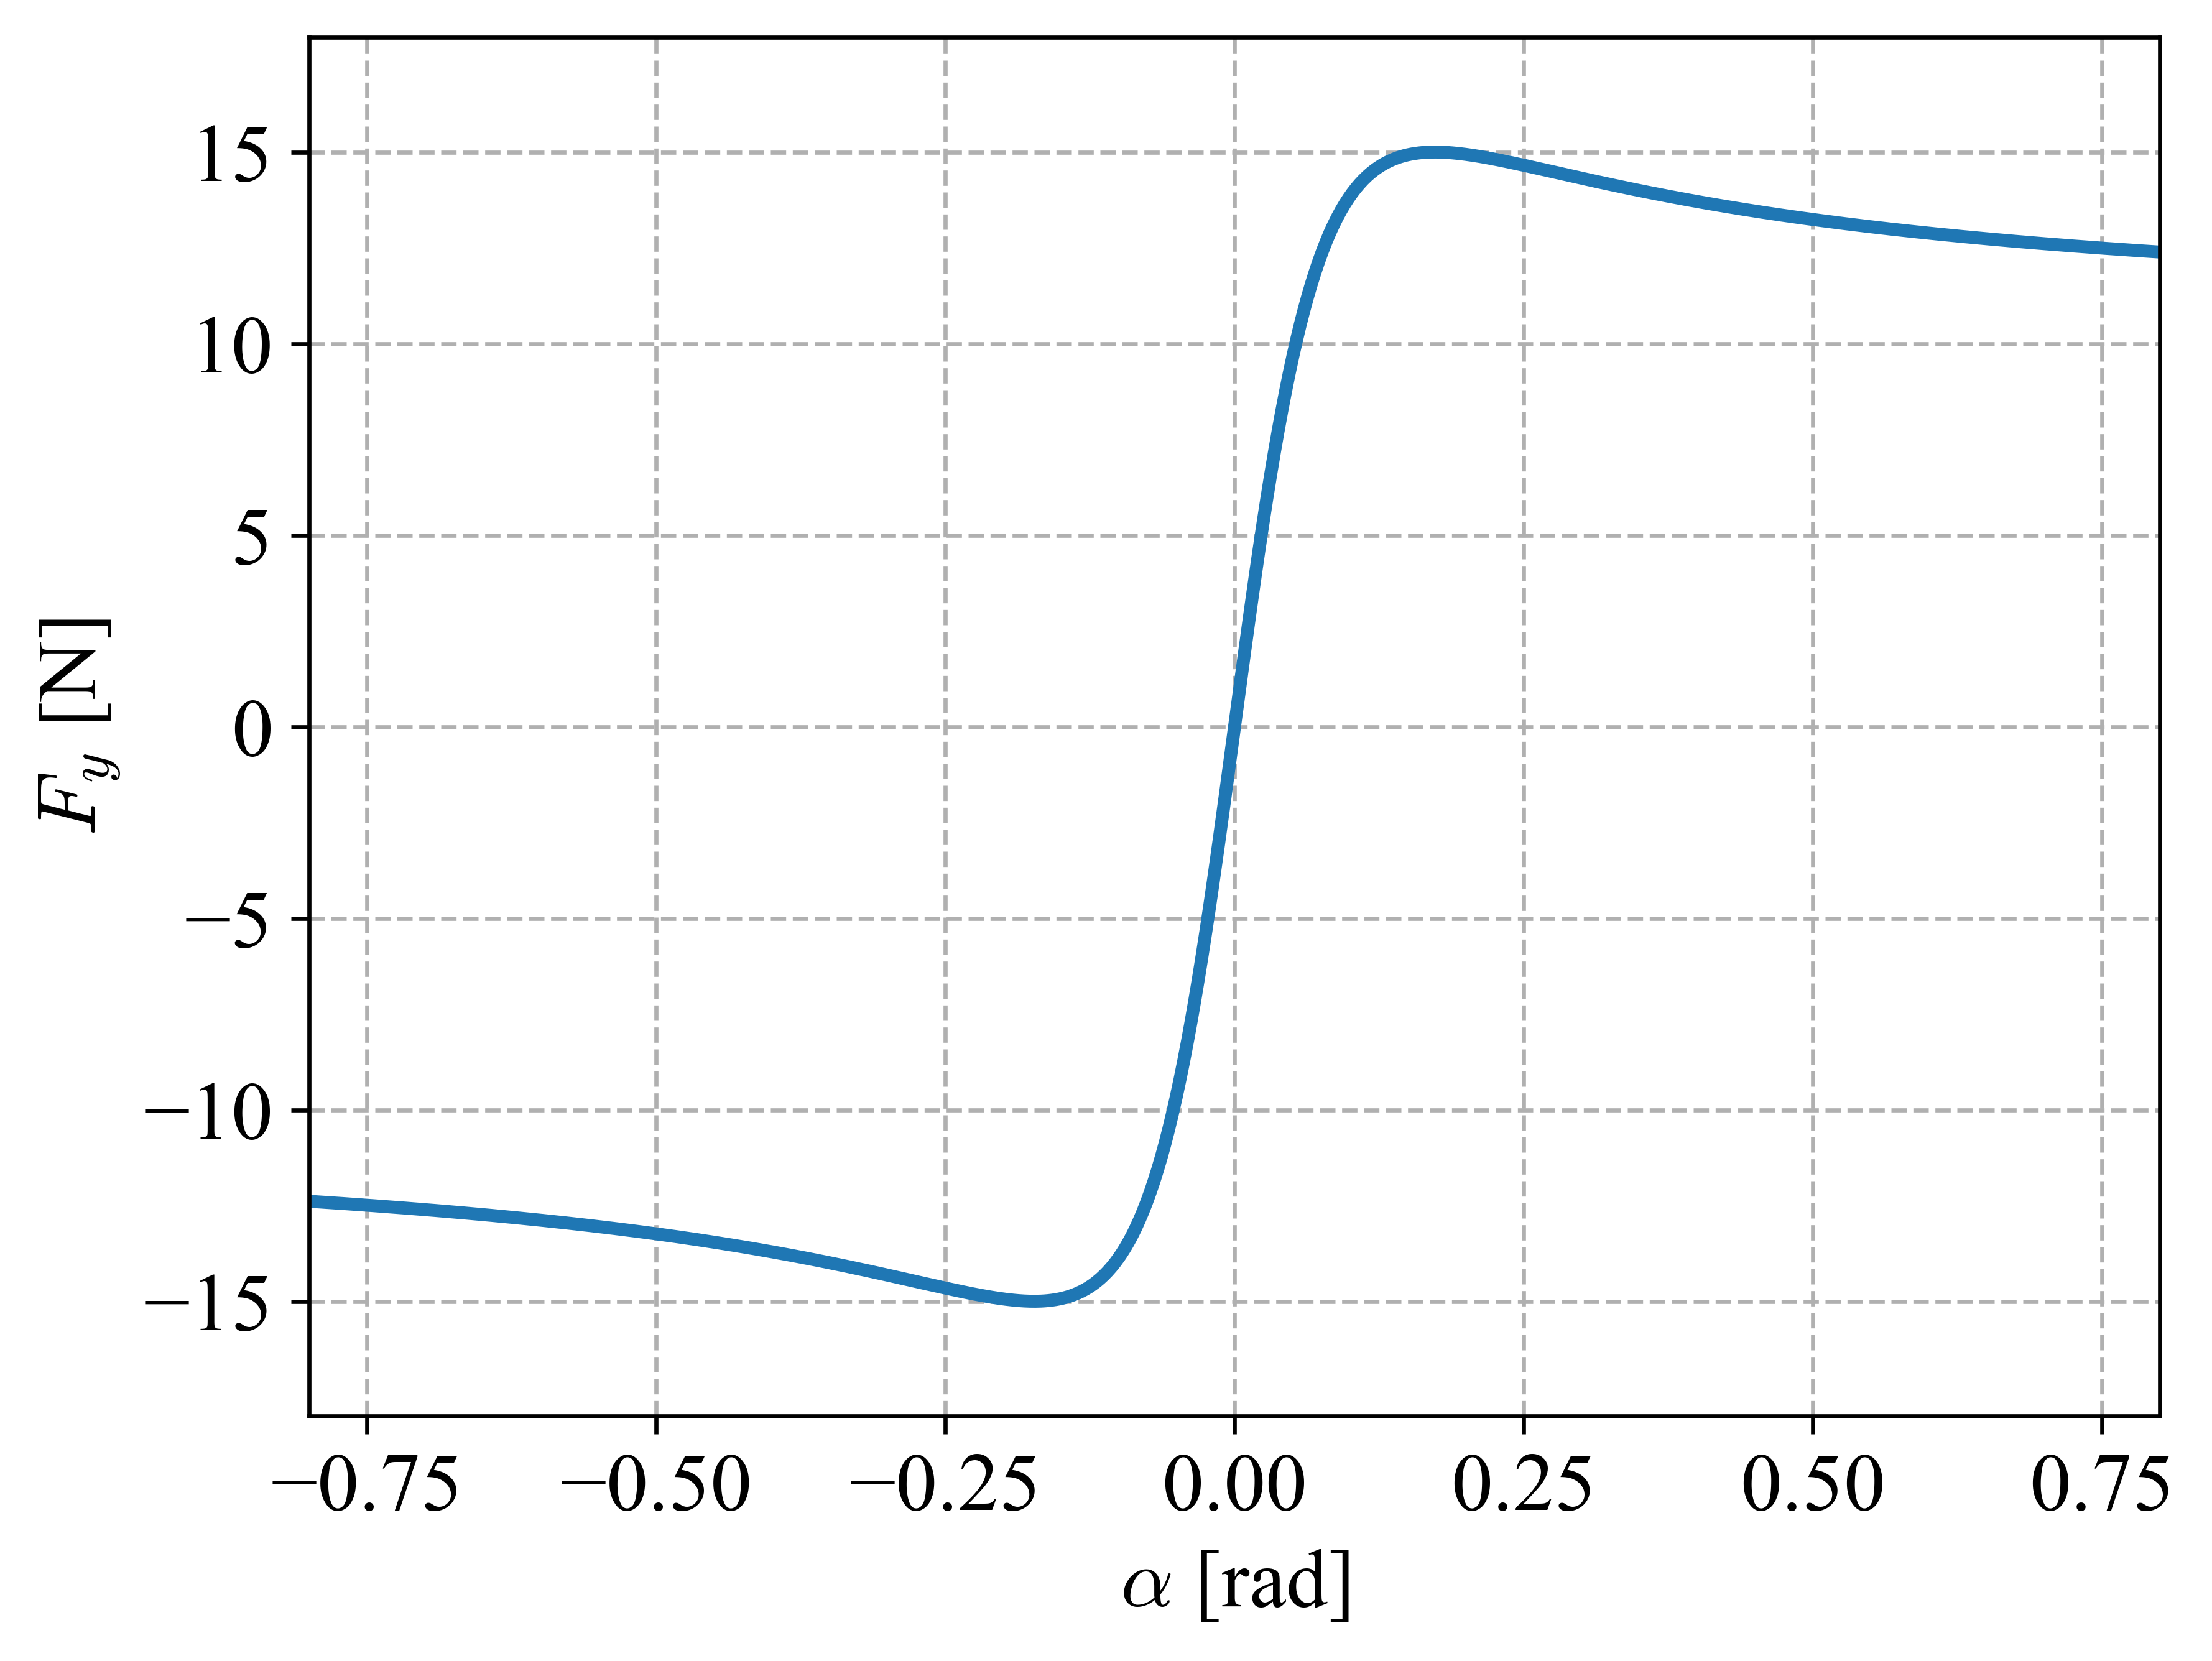
\includegraphics[width=0.55\linewidth]{figure/chapter2/magic.png}
    \caption{魔术公式曲线示例：$B=10$，$C=1.5$，$D=15$，$E=0.1$}
    \label{fig:magic-formula}
\end{figure}

为了计算方便，我们令$E=0$，从而简化魔术公式模型的表达式:
\begin{equation}
\begin{aligned}
    F_{y,i}(\alpha_i)=D_i\sin{(C_i\arctan{(B_i\alpha_i)})},i\in\{f,r\}.
\end{aligned}
\end{equation}
简化后的魔术公式模型仍然能够较好地描述轮胎的横向力特性，并且减少了模型的复杂度，便于后续的控制设计和参数辨识。

另外，车辆的纵向驱动力$F_x$可以通过后轮的驱动输入$T$和轮胎的摩擦特性计算得到。具体来说，$F_x$可以表示为：
\begin{equation}
\begin{aligned}
    F_x=C_m T-C_d - C_v v_x^2,
\end{aligned}
\end{equation}
其中$C_m$是驱动增益，$C_d$是滚动阻力系数，$C_v$是空气阻力系数。通过调整这些参数，我们可以模拟不同的驱动和阻力特性，从而更准确地描述车辆的纵向动力学行为。

综上所述，赛车的完整动力学模型为：
\begin{equation}
\begin{aligned}
    \dot{\boldsymbol{x}}=f(\boldsymbol{x}, \boldsymbol{u})=\left[ \begin{matrix}
        v_x\cos{\phi}-v_y\sin{\phi}  \\
        v_x\sin{\phi}+v_y\cos{\phi}  \\
        \omega  \\
        \frac{1}{m}(F_x-F_{y,f}\sin{\delta}+mv_y\omega)  \\
        \frac{1}{m}(F_{y,r}+F_{y,f}\cos{\delta}-mv_x\omega)  \\
        \frac{1}{I_z}(F_{y,f}l_f\cos{\delta}-F_{y,r}l_r)  \\
    \end{matrix} \right].
\end{aligned}
\label{equ:car-fulldynamics}
\end{equation}

\subsection{动力学参数辨识}
为了确保动力学模型能够准确地描述赛车的运动行为，我们需要对模型中的关键参数进行辨识。模型中的参数主要分为两类：车辆参数和轮胎参数。车辆参数包括质量$m$、偏航转动惯量$I_z$、前轴和后轴到质心的距离$l_f$和$l_r$等；轮胎参数包括魔术公式模型中的参数$B$、$C$、$D$和$E$，以及纵向动力学中的驱动增益$C_m$、滚动阻力系数$C_d$和空气阻力系数$C_v$。其中，车辆参数可以通过直接测量获得，而轮胎参数则需要通过实验数据进行辨识。本文所用到的车辆参数如表\ref{table:car-params}所示。
\begin{table}[ht]
\renewcommand{\arraystretch}{1.25}
\caption{\label{table:car-params}本文所用赛车的车辆参数}
\begin{tabularx}{\linewidth}{X<{\centering} X<{\centering} X<{\centering}}
        \toprule[2pt]
        参数 & 单位 & 大小 \\ \midrule[1pt]
        赛车质量$m$ & kg & 3.93 \\
        偏航转动惯量$I_z$ & kg·m² & 0.0383 \\
        前轴到质心的距离$l_f$ & m & 0.18 \\
        后轴到质心的距离$l_r$ & m & 0.14 \\
        \bottomrule[2pt]
    \end{tabularx}
\end{table}
其中，车辆的质量$m$通过称重获得，前轴和后轴到质心的距离$l_f$和$l_r$通过测量车辆的几何尺寸获得，偏航转动惯量$I_z$则通过假设赛车为一个均匀分布的矩形平板来近似计算得到：
\begin{equation}
\begin{aligned}
    I_z=\frac{1}{12}m(l^2+w^2),
\end{aligned}
\end{equation}
其中$l$和$w$分别表示赛车的长度和宽度。

对于轮胎参数的辨识，我们通过在不同工况下进行车辆测试，收集车辆的状态和控制输入数据，并使用非线性优化方法拟合魔术公式模型的参数。具体来说，我们通过调整参数$B$、$C$、$D$和$E$，使得模型预测的轮胎力与实验数据中的轮胎力尽可能匹配，从而获得了准确的轮胎参数。为了尽可能地覆盖不同的工况，本文设计了如图\ref{fig:iden-traj}所示的参数辨识轨迹，该轨迹包含了不同速度、转向角和加速度的组合，以确保参数辨识的全面性和准确性。在收集数据时，采用PID控制器来跟踪预设的轨迹，并记录车辆的状态和控制输入数据。
\begin{figure}[ht]
    \centering
    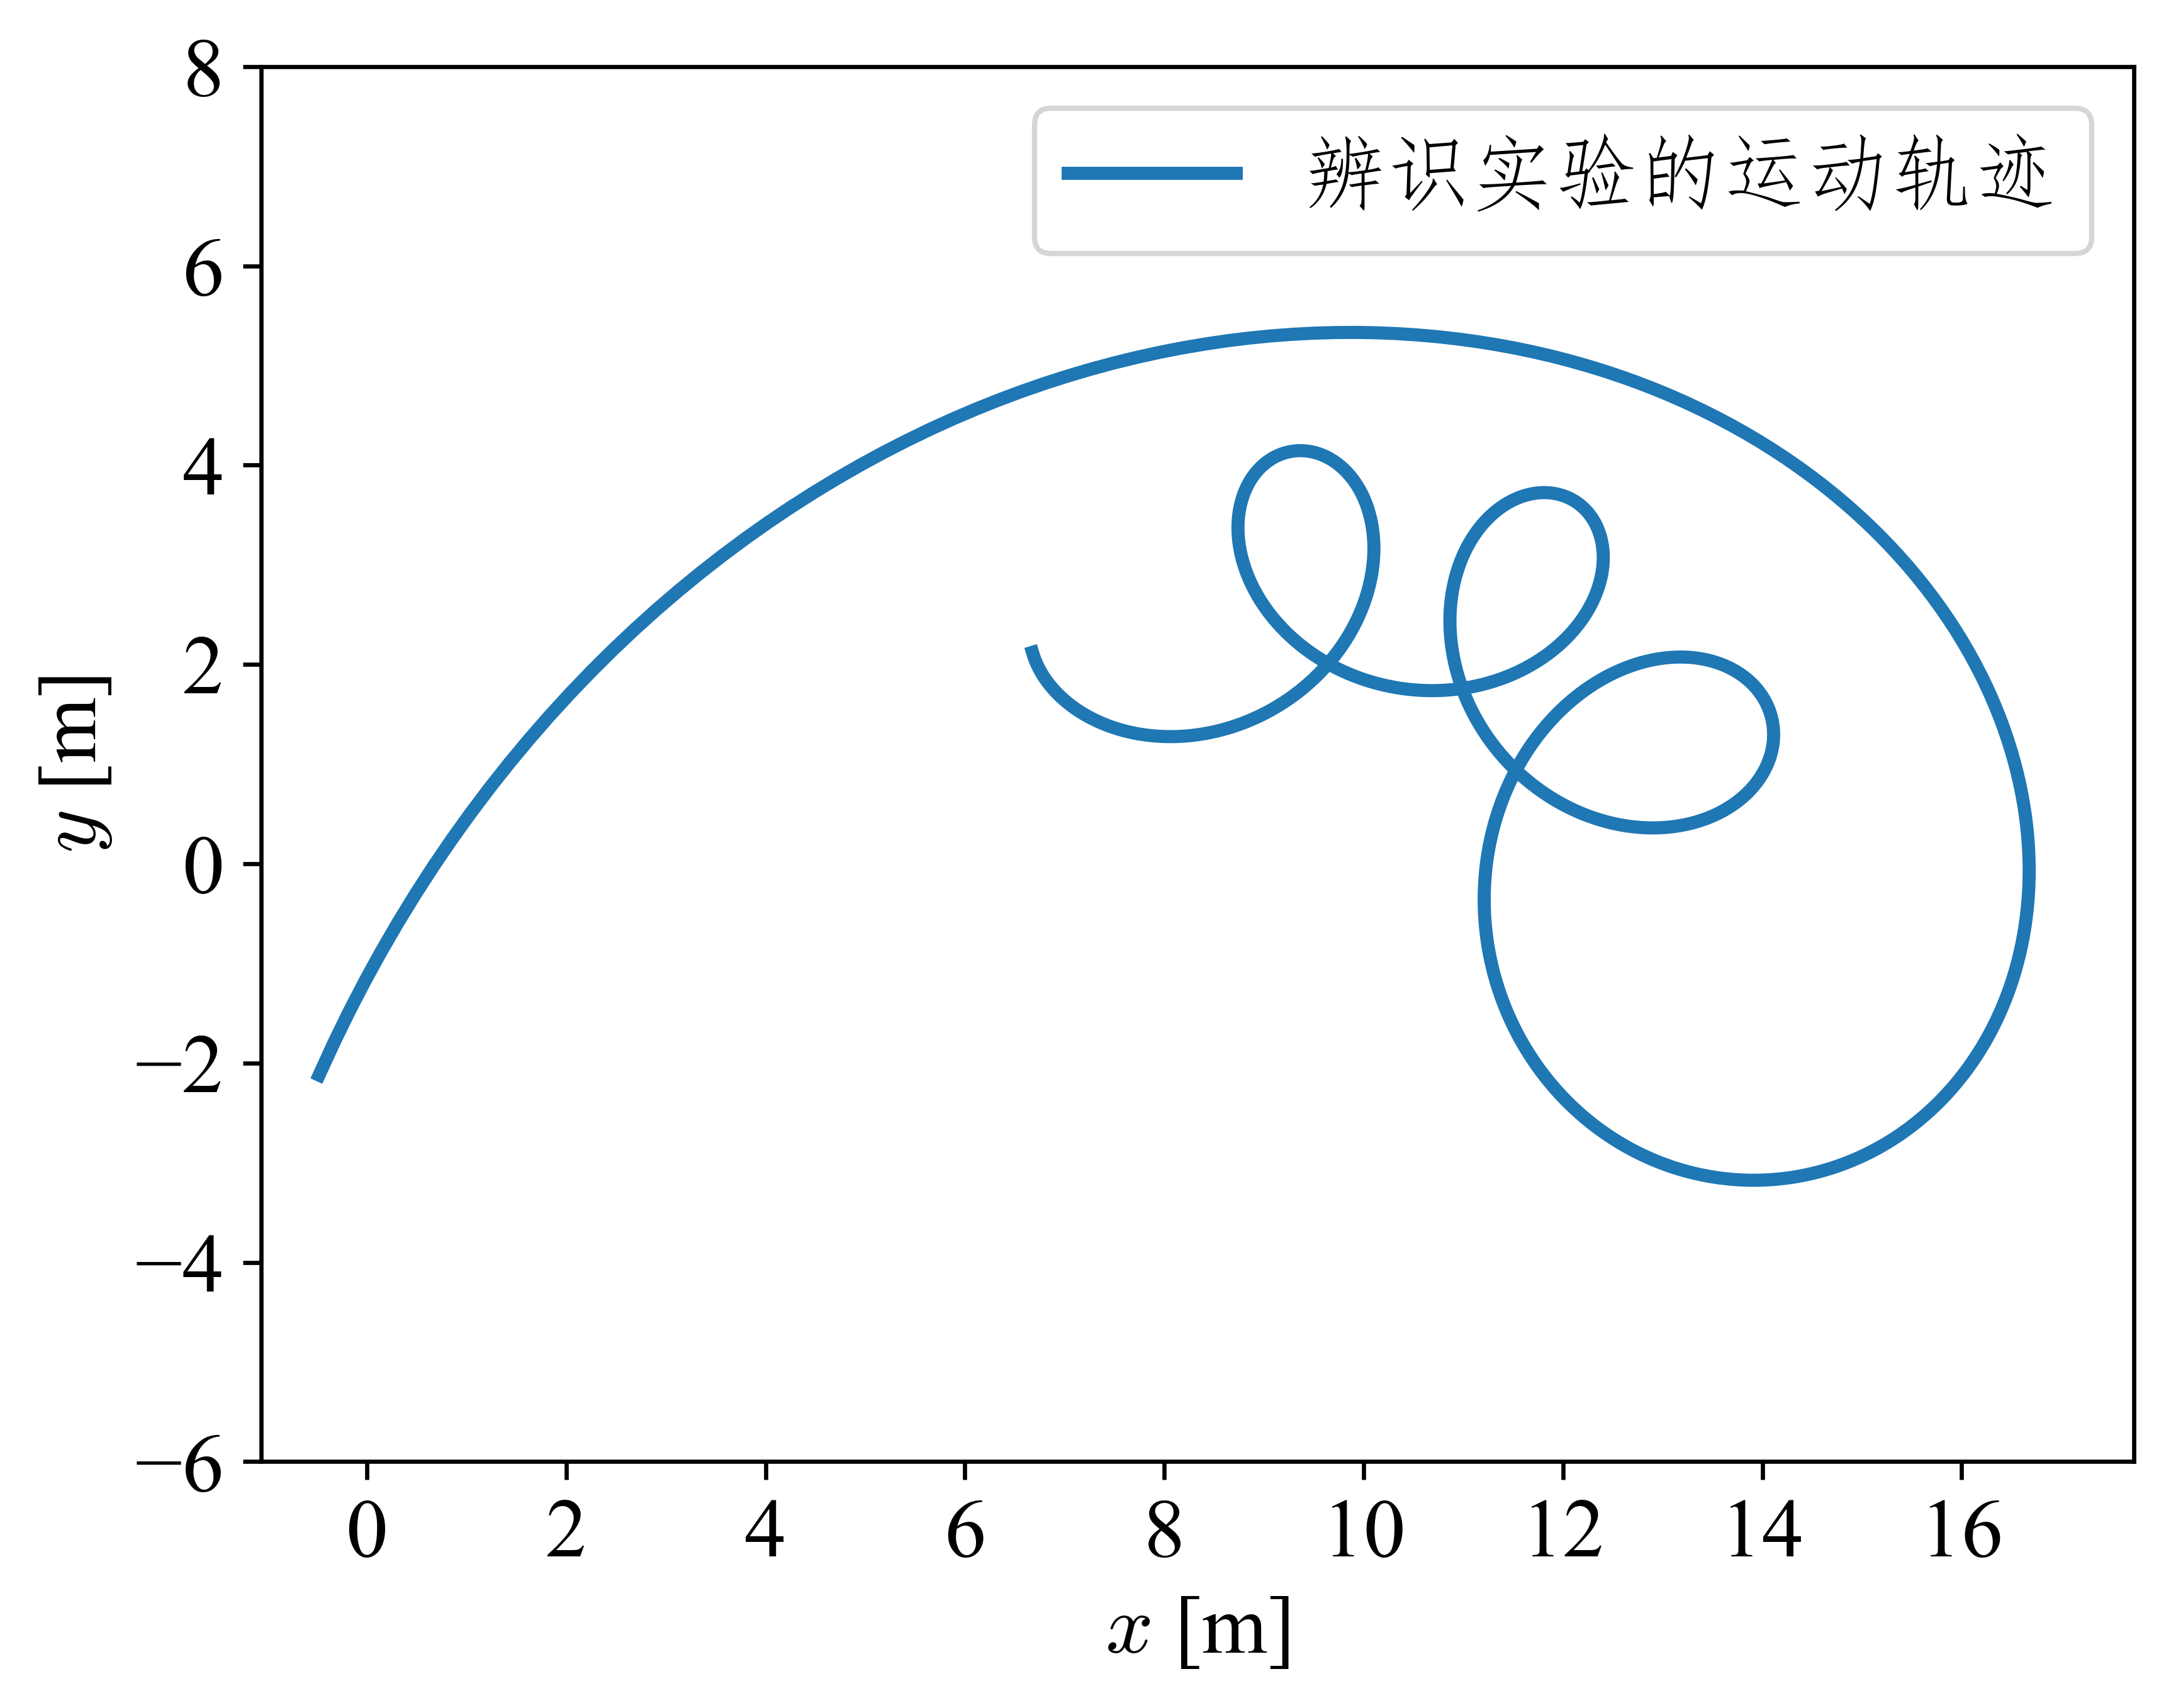
\includegraphics[width=0.6\linewidth]{figure/chapter2/iden-traj.png}
    \caption{轮胎参数辨识轨迹}
    \label{fig:iden-traj}
\end{figure}

根据公式（\ref{equ:car-dynamics}）可得轮胎侧向力$F_{y,f}$和$F_{y,r}$的计算方法：
\begin{equation}
\begin{aligned}
    F_{y,f}&=\frac{m\dot{v_y}l_r + m v_x\omega l_r + \dot{\omega}I_z}{(l_f+l_r)\cos{\delta}},\\
    F_{y,r}&=\frac{m\dot{v_y}l_f + m v_x\omega l_f - \dot{\omega}I_z}{l_f+l_r}.
\end{aligned}
\label{equ:tire-forces}
\end{equation}
由此可知辨识轮胎参数需要获取车辆的状态数据$\dot{v_y}$、$v_x$、$\omega$和$\dot{\omega}$，以及控制输入数据$\delta$。其中，$\dot{v_y}$和$\omega$可以通过安装在车辆上的IMU传感器测量得到，IMU传感器中的噪声使用低通滤波器来消除，截止频率为30Hz；$\dot{\omega}$可以通过对$\omega$进行数值微分得到，同样需要进行滤波处理以减少噪声的影响；$v_x$则使用IMU传感器提供的加速度和角速度与动作捕捉系统提供的位置与姿态信息进行拓展卡尔曼滤波（Extended Kalman Filter，简称EKF）融合计算得到；$\delta$可以通过记录控制输入数据获得。根据公式（\ref{equ:tire-forces}）计算得到轮胎侧向力后可进行最小二乘拟合来辨识魔术公式模型中的参数$B$、$C$、$D$：
\begin{equation}
\begin{aligned}
    \min_{B_{f/r},C_{f/r},D_{f/r}} \quad & \frac{1}{N}\sum_{j=1}^{N}(F_{y,f/r}^j-D_{f/r}\sin{(C_{f/r}\arctan{(B_{f/r}\alpha_{f/r}^j)})})^2,\\
    \text{s.t.} \quad & B_{f/r}>0, C_{f/r}>0, D_{f/r}>0,
\end{aligned}
\end{equation}
其中，$N$为采样点的数量，$F_{y,f/r}^j$为第$j$个采样点计算得到的轮胎侧向力，$\alpha_{f/r}^j$为第$j$个采样点计算得到的轮胎侧偏角，由公式（\ref{equ:slip-angle}）计算得到。通过求解上述优化问题，我们可以获得准确的轮胎参数，从而使得动力学模型能够更好地描述赛车的运动行为。图\ref{fig:tire-iden}展示了前轮和后轮侧向力的参数辨识结果示例。
\begin{figure}[ht]
    \centering
    \subfloat[前轮侧向力的参数辨识结果]{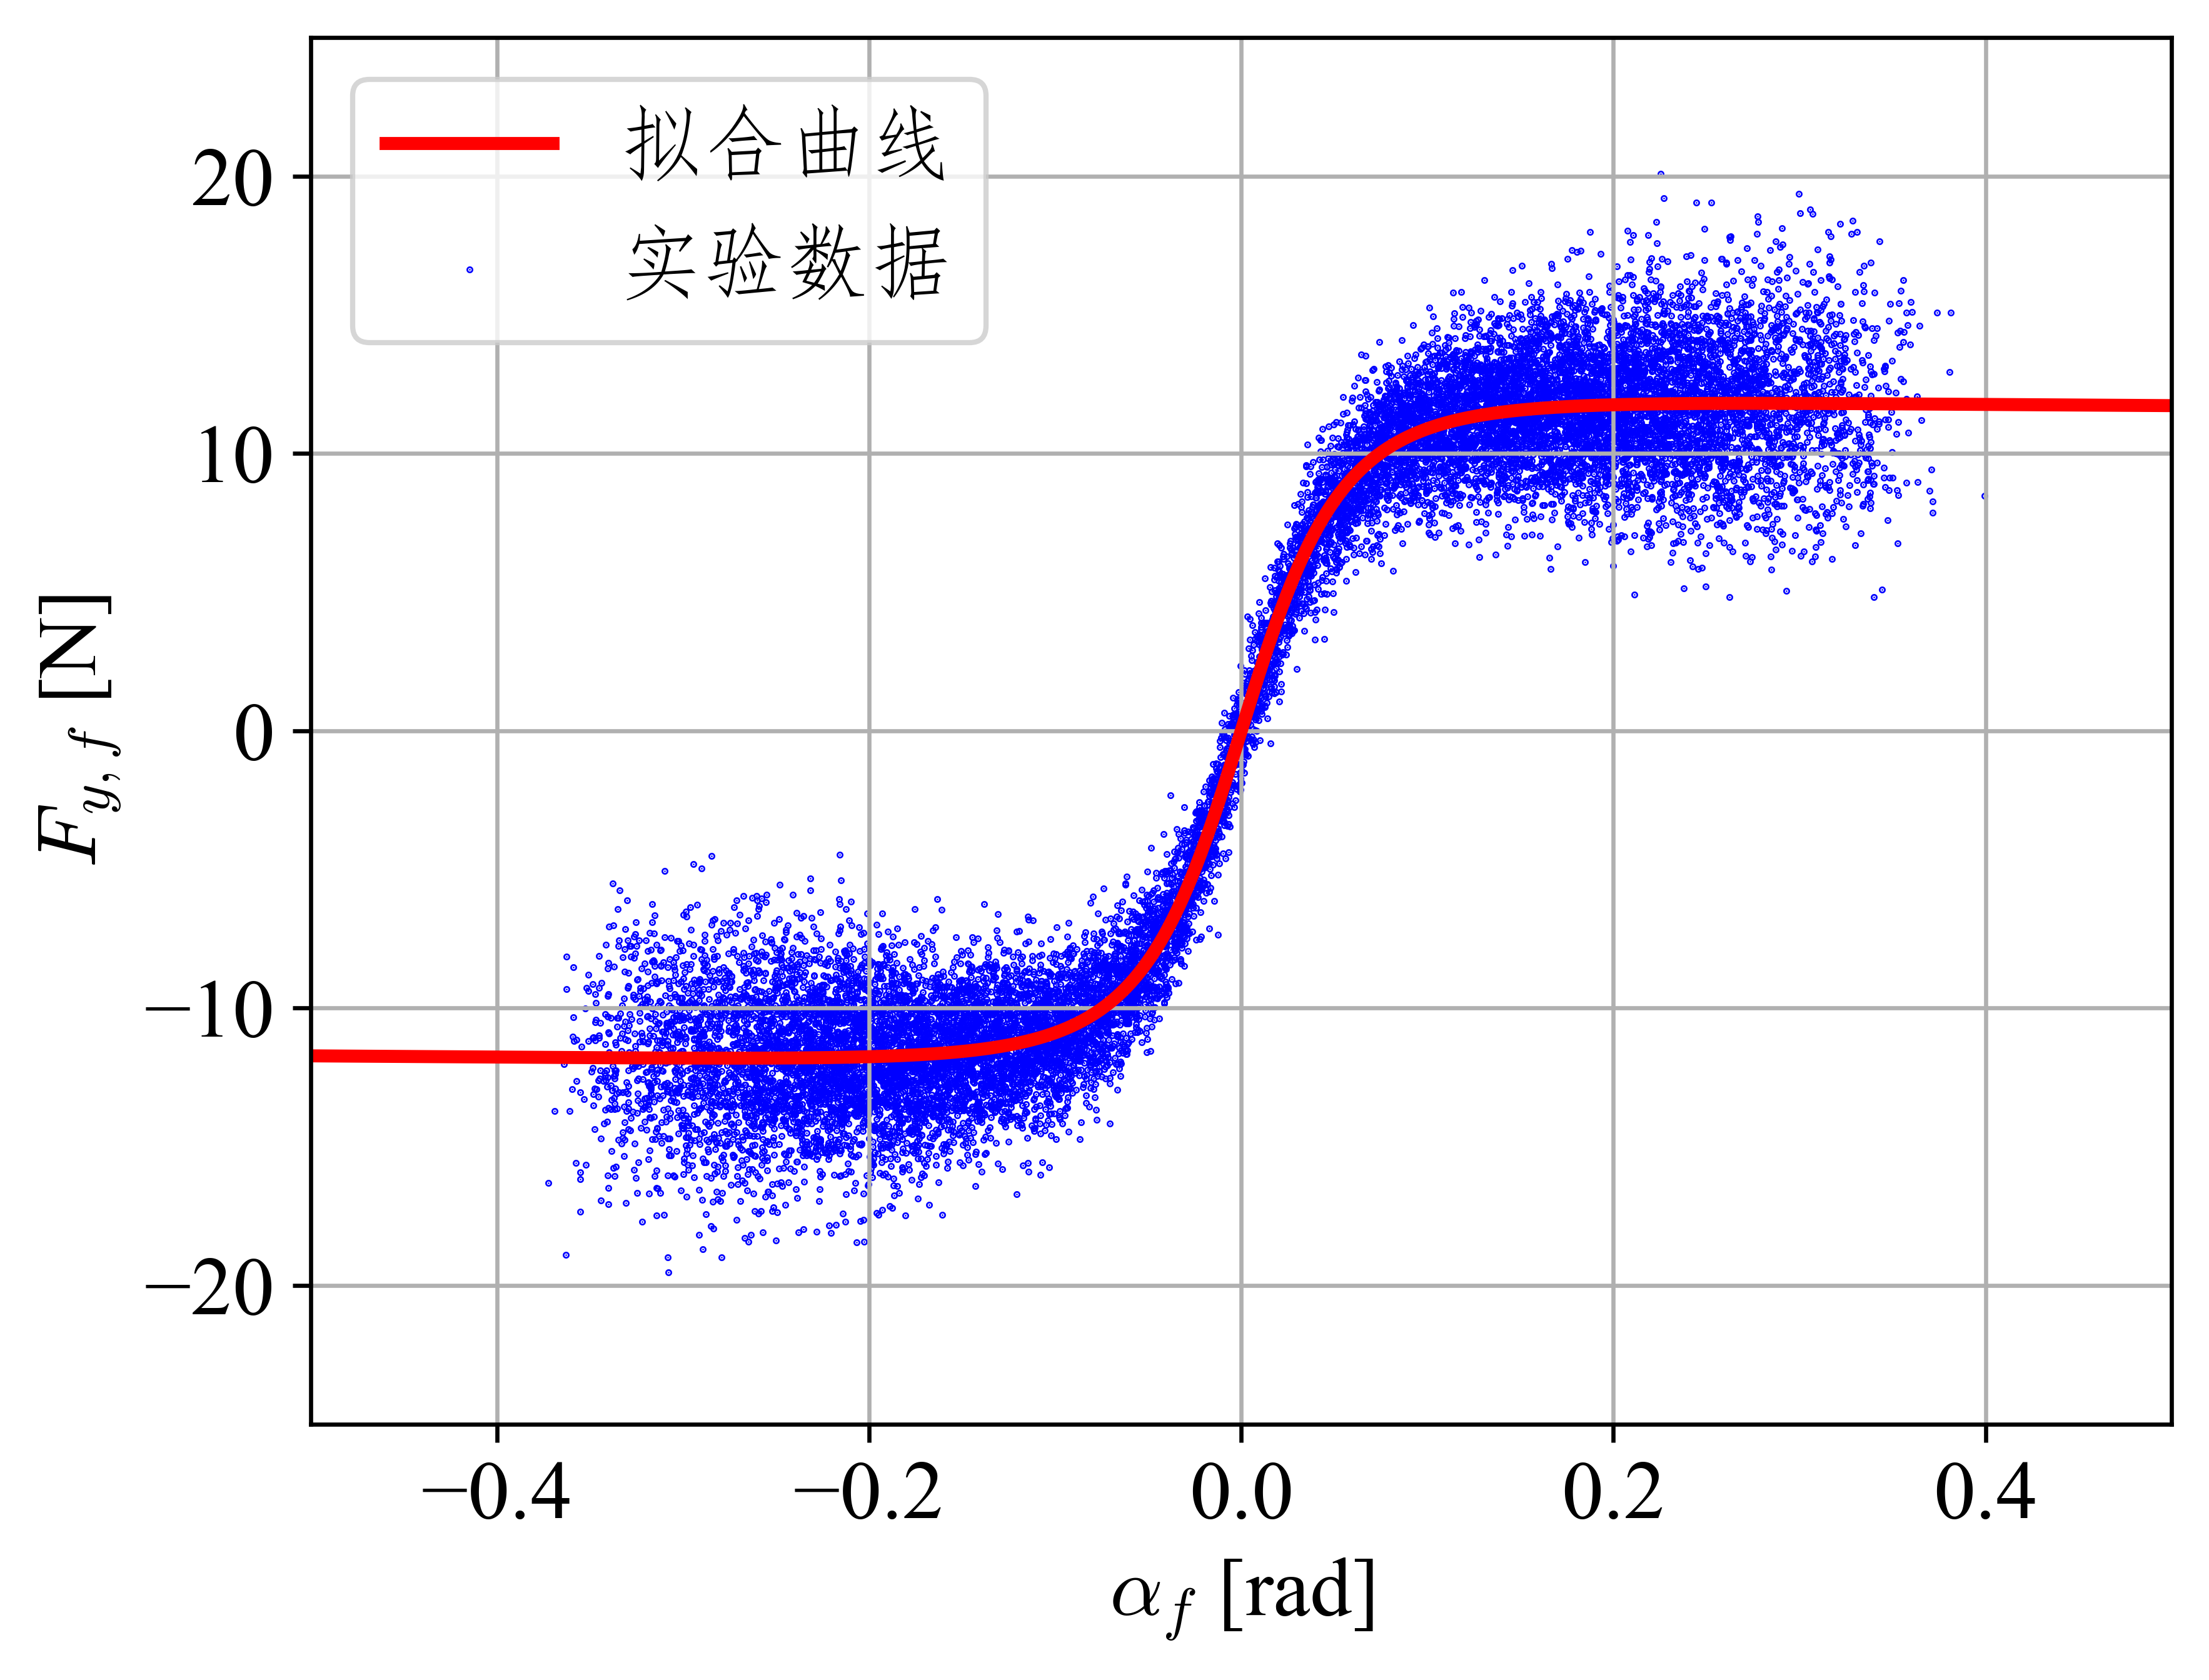
\includegraphics[width=0.45\linewidth]{figure/chapter2/tire-figure-front.png}}
    \subfloat[后轮侧向力的参数辨识结果]{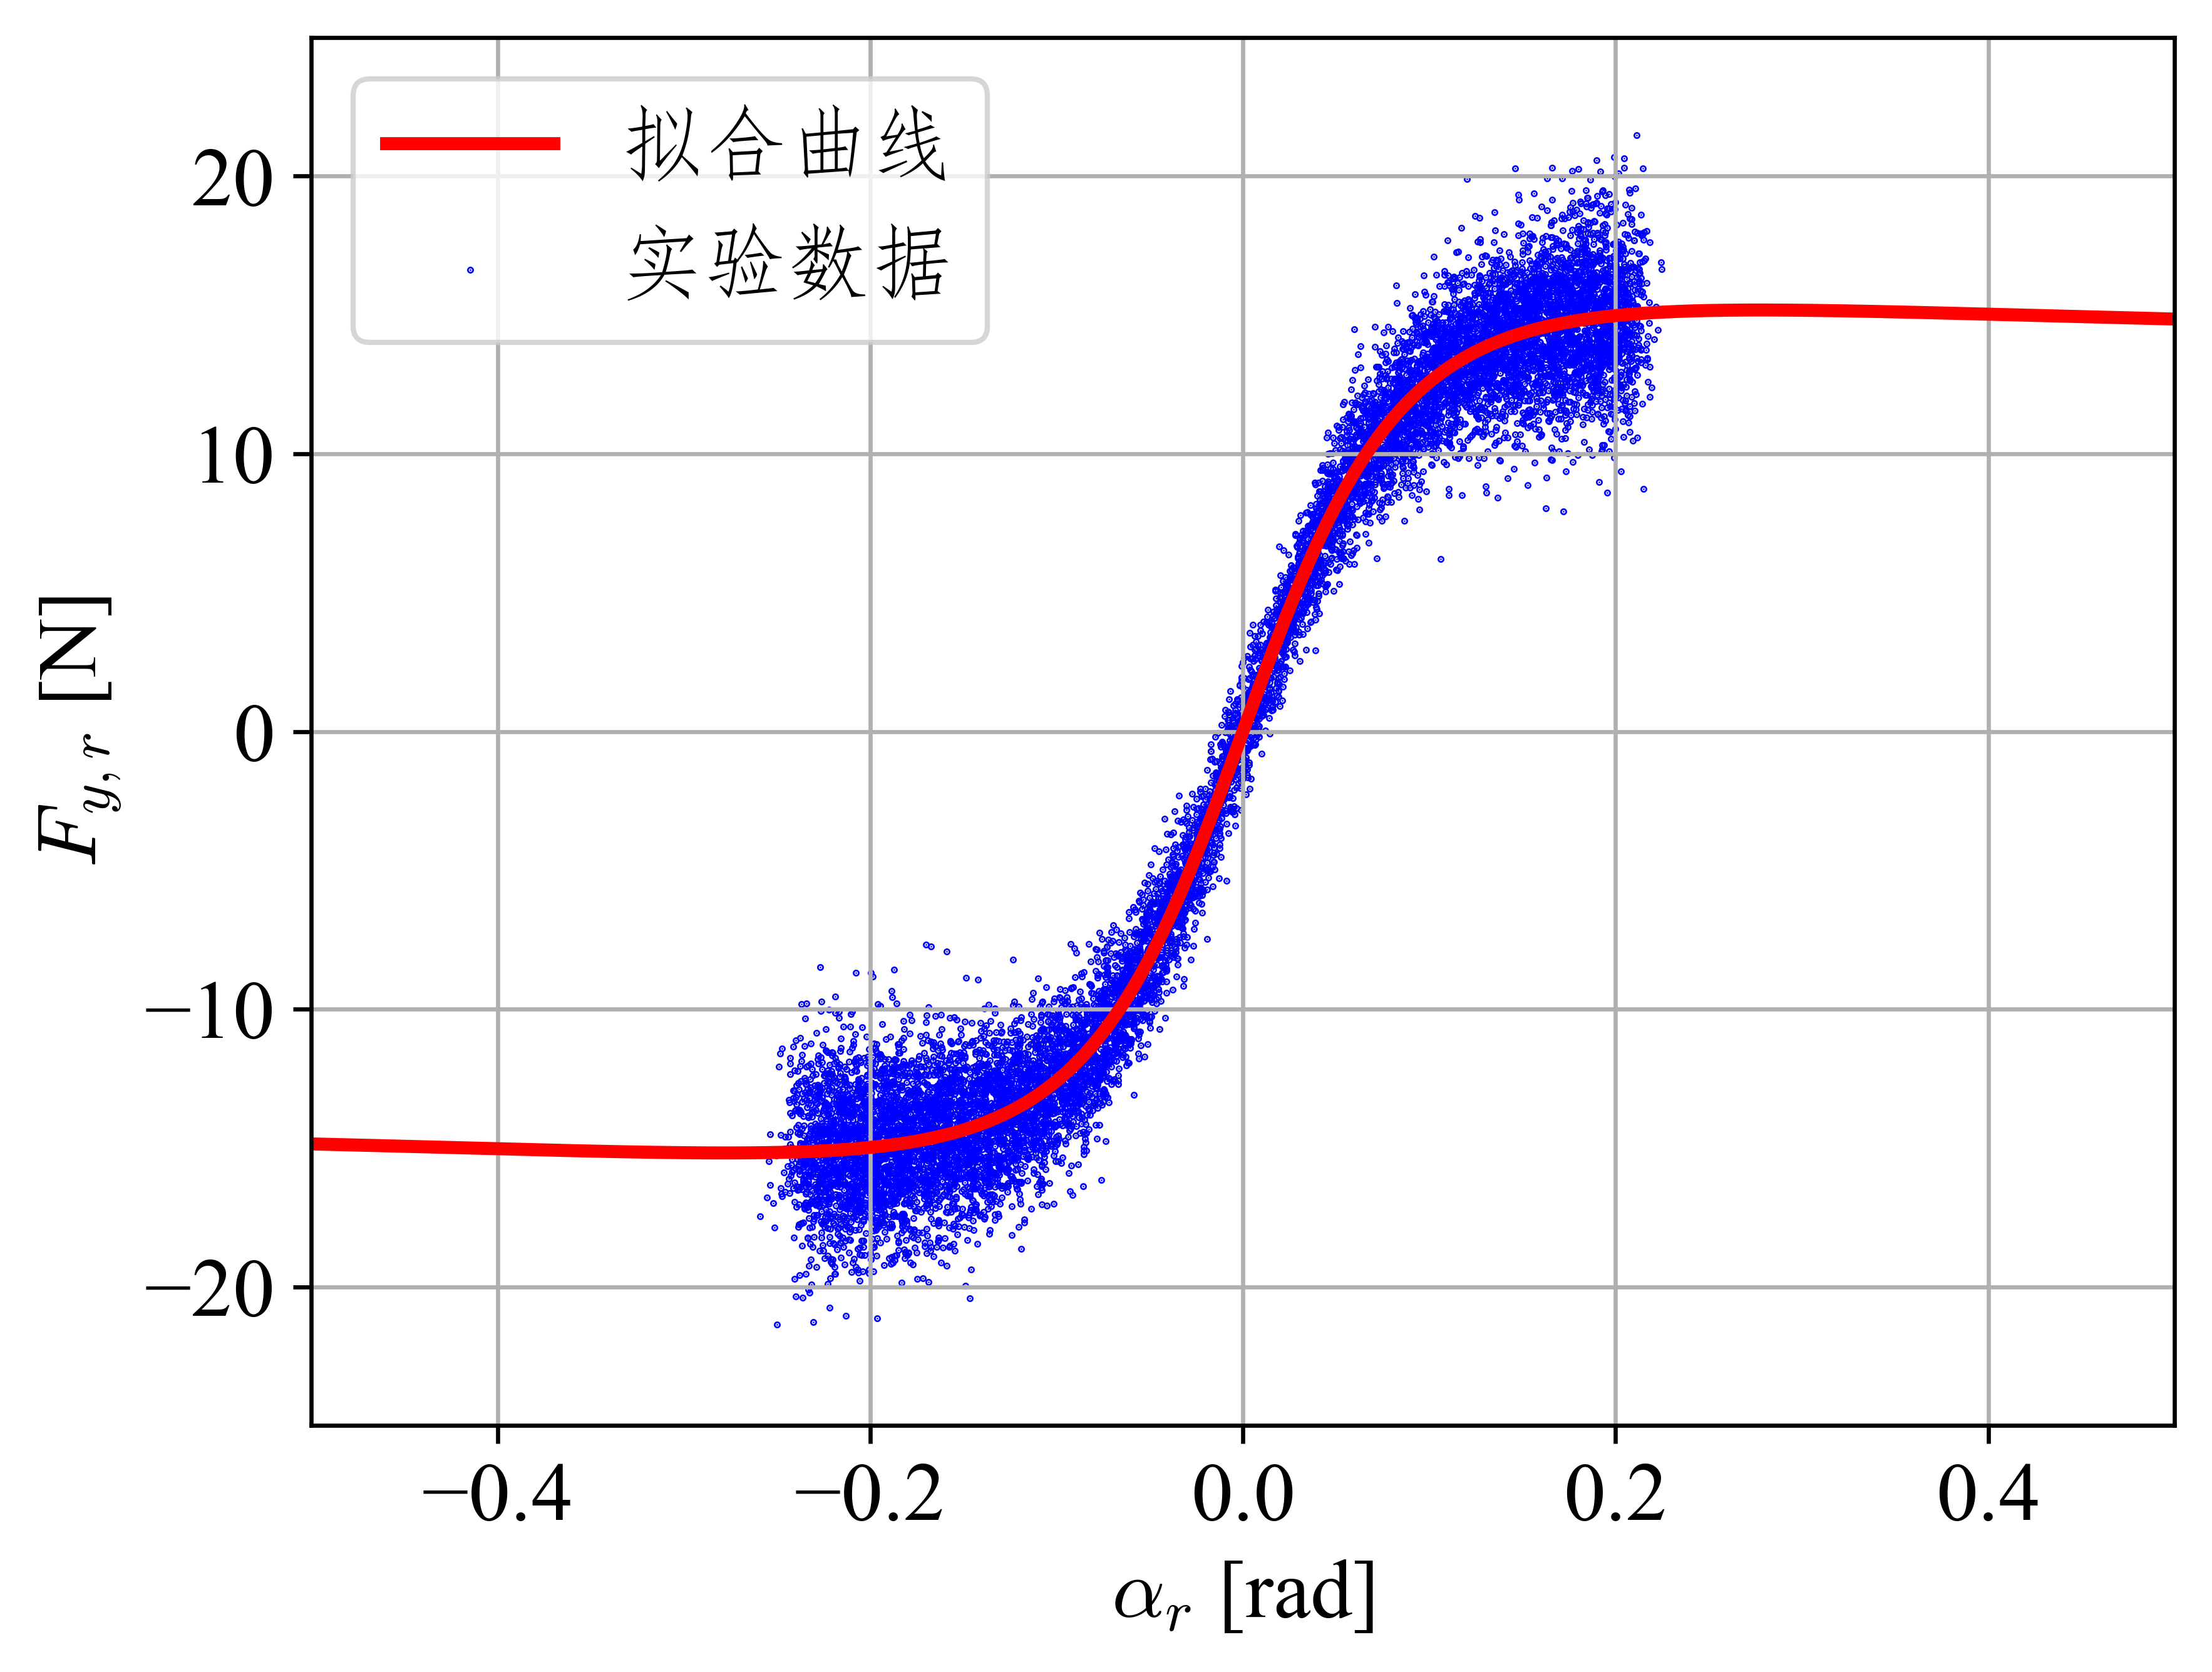
\includegraphics[width=0.45\linewidth]{figure/chapter2/tire-figure-rear.png}}
    \caption{轮胎参数辨识结果}
    \label{fig:tire-iden}
\end{figure}

对于驱动力参数的辨识，我们通过采集赛车直线行驶的数据来辨识驱动增益$C_m$、滚动阻力系数$C_d$和空气阻力系数$C_v$。具体来说，我们让赛车在平坦的赛道上以不同的油门输入进行直线加速和减速，并记录车辆的纵向速度$v_x$、IMU传感器数据滤波得到的加速度$\dot{v_x}$和驱动输入$T$。此时车辆的横向运动可以忽略，即$v_y\approx 0$，$\omega\approx 0$，$\delta\approx 0$，根据公式（\ref{equ:car-dynamics}）可得车辆的纵向加速度$\dot{v_x}$与驱动力$F_x$的关系为：
\begin{equation}
\begin{aligned}
    F_x=m\dot{v_x}.
\end{aligned}
\end{equation}
因此，我们可以通过拟合车辆的纵向加速度与驱动输入之间的关系来辨识驱动力参数。具体来说，我们可以通过最小二乘拟合来求解以下优化问题：
\begin{equation}
\begin{aligned}
    \min_{C_m,C_d,C_v} \quad & \frac{1}{N}\sum_{j=1}^{N}(F_x^j-(C_m T^j-C_{d} - C_v (v_x^j)^2))^2,\\
    \text{s.t.} \quad & C_m>0, C_d>0, C_v>0,
\end{aligned}
\end{equation}
其中，$N$为采样点的数量，$F_x^j$为第$j$个采样点计算得到的纵向驱动力，$T^j$为第$j$个采样点的驱动输入，$v_x^j$为第$j$个采样点的纵向速度。图\ref{fig:drive-iden}展示了驱动力参数辨识的结果示例，我们恒定油门输入$T=0.5$，让赛车在平坦的赛道上进行直线加速，并记录车辆的纵向速度，将其与辨识出的模型进行比较，可以看出辨识出的模型能够较好地拟合车辆的纵向加速行为，从而验证了驱动力参数辨识的有效性。
\begin{figure}[ht]
    \centering
    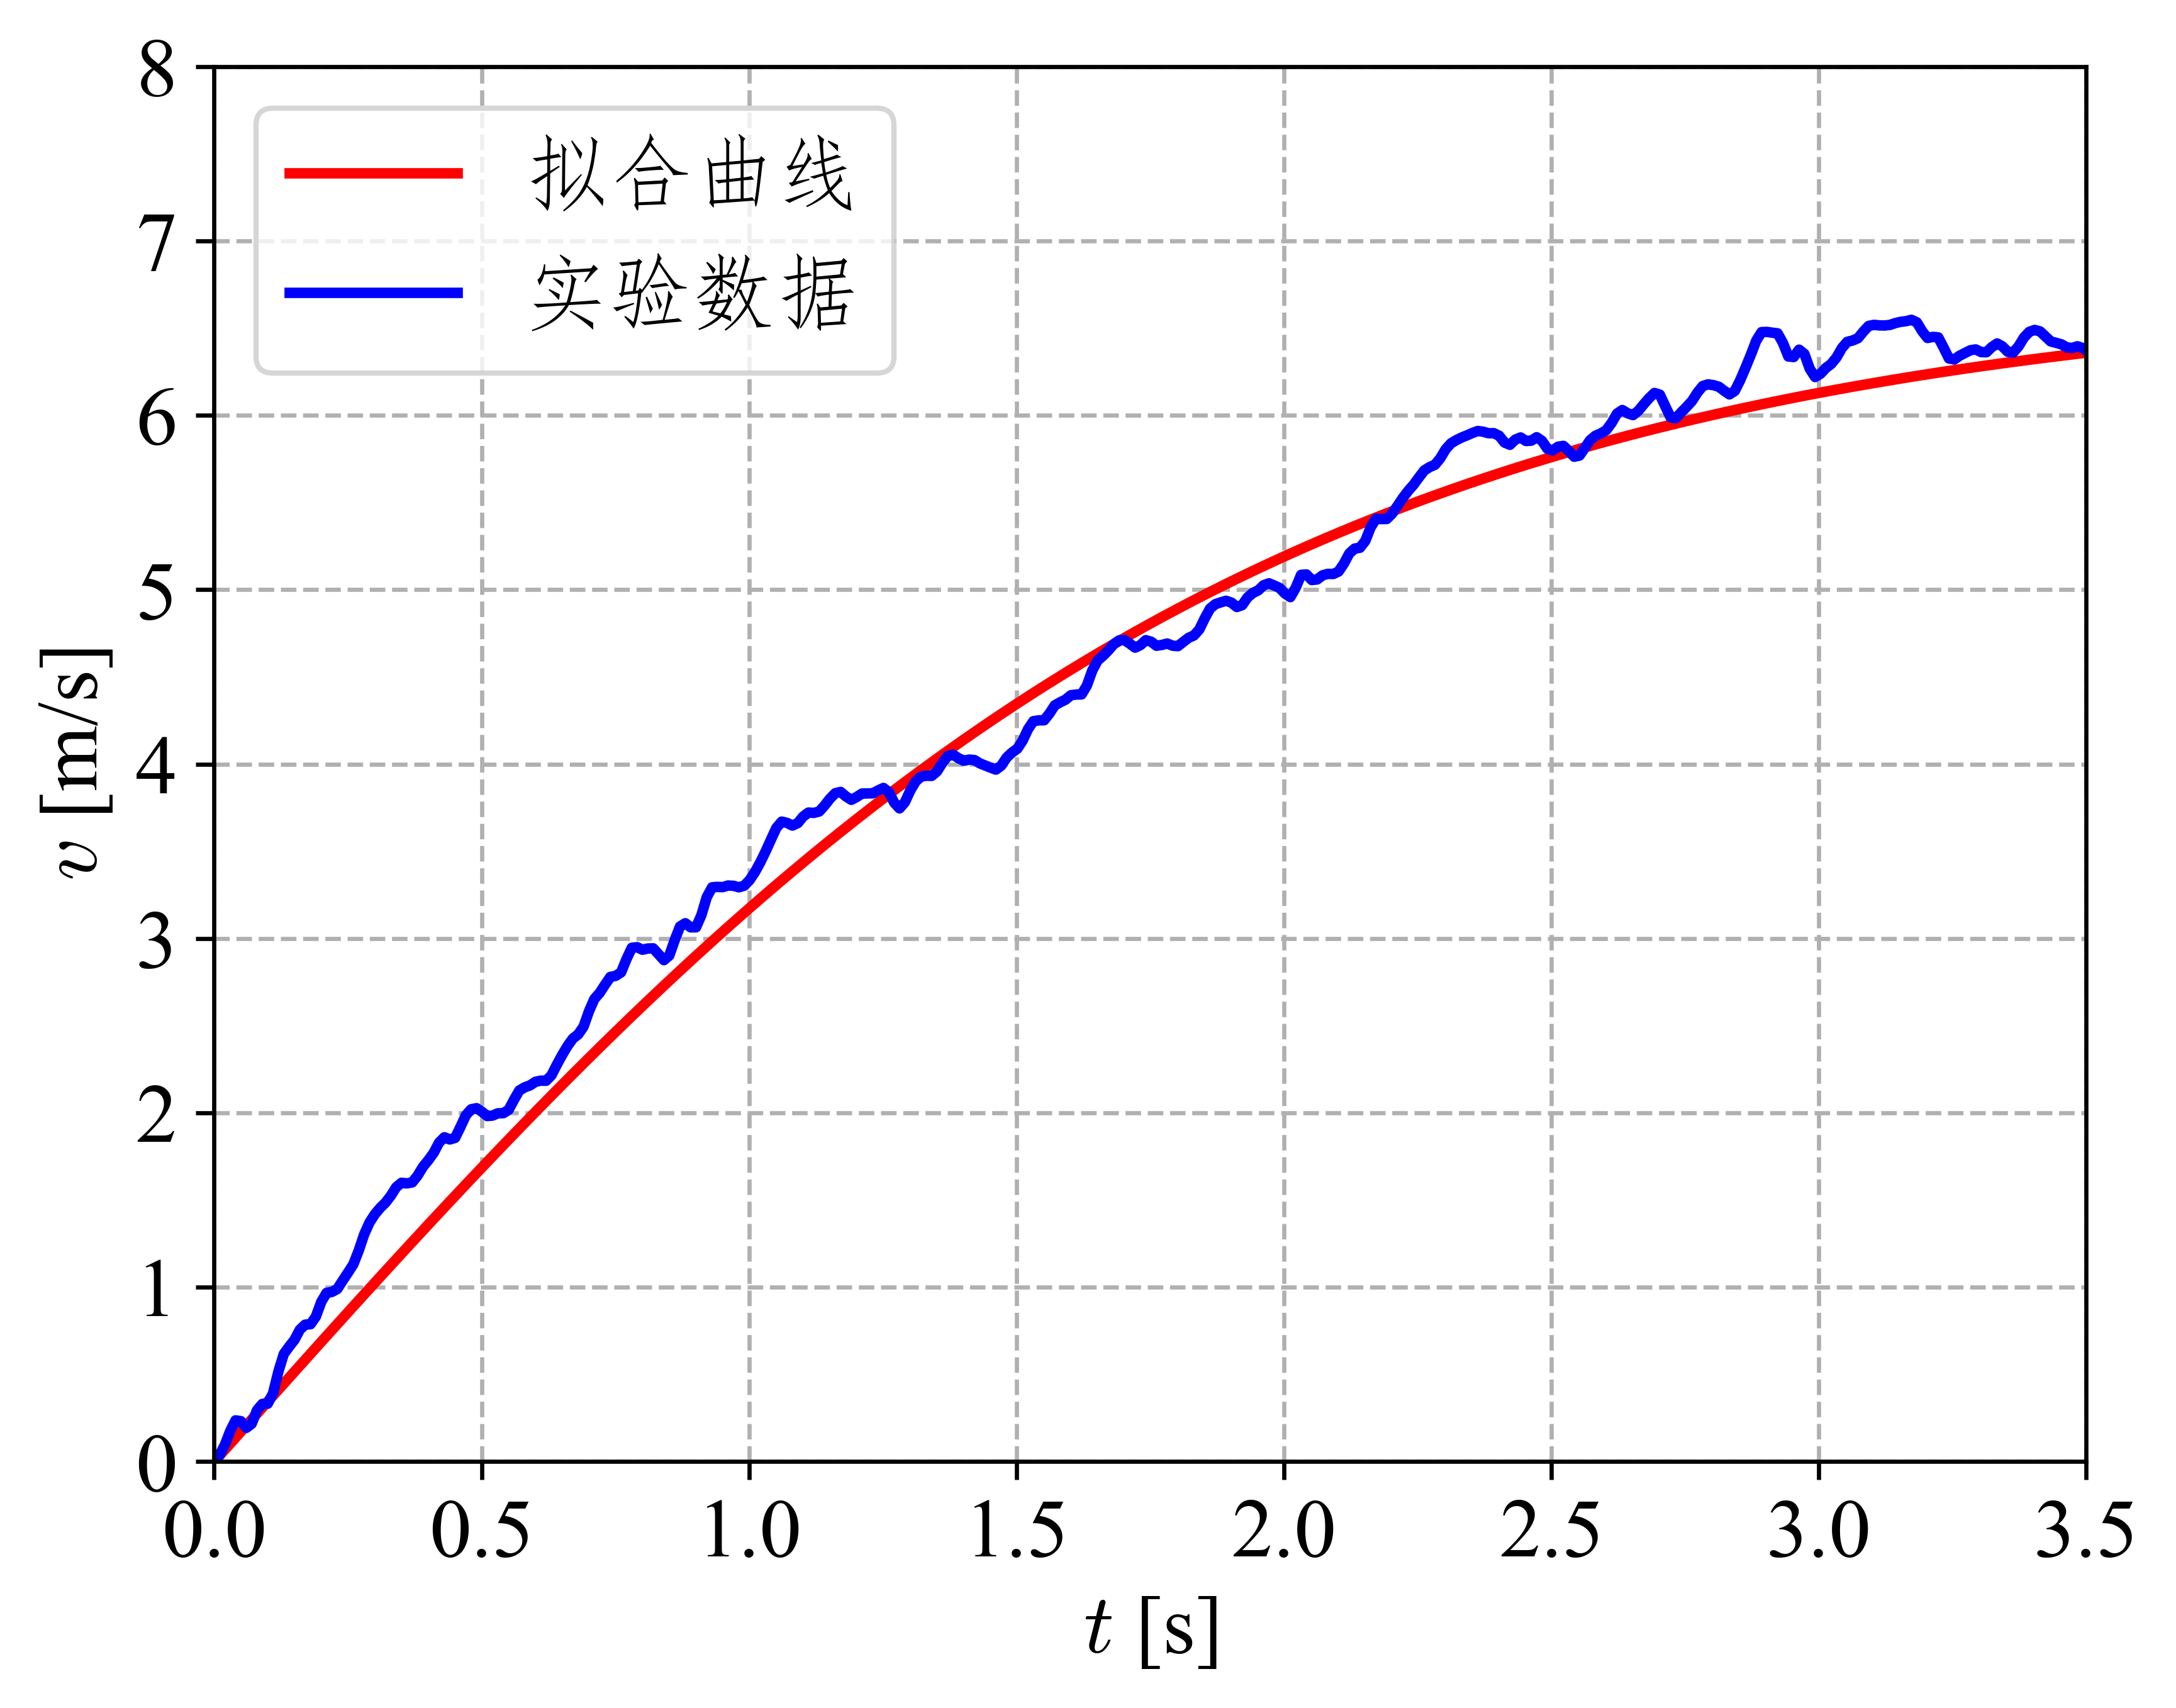
\includegraphics[width=0.5\linewidth]{figure/chapter2/drive-iden.png}
    \caption{驱动力参数辨识结果示例}
    \label{fig:drive-iden}
\end{figure}

综上，轮胎与驱动的参数辨识的结果如表\ref{tab:dyna-param-iden}所示：
\begin{table}[h]
    \caption{\label{tab:dyna-param-iden}赛车平台动力学参数辨识结果}
    \renewcommand\arraystretch{1.25}
    \begin{tabularx}{\linewidth}{X<{\centering} X<{\centering} || X<{\centering} X<{\centering}}
        \Xhline{2pt}
        % \toprule[2pt]
        参数    & 辨识结果 & 参数  & 辨识结果 \\ \Xhline{1pt}
        $C_m$     & 30.17    & $B_f$ & 15.7     \\
        $C_d$     & 1.49    & $C_f$ & 1.17     \\
        $C_v$     & 0.31   & $B_r$ & 9.24     \\
        $D_f$ & 11.81     & $C_r$ & 1.31     \\
        $D_r$ & 15.34     &       &          \\ \Xhline{2pt}
        % \Xhline{2-3}{0.4pt}
    \end{tabularx}
\end{table}


\section{基于控制障碍函数的安全竞速控制}
\subsection{控制障碍函数介绍与可行性分析}
控制障碍函数（Control Barrier Function，简称CBF）是一种用于确保系统安全性的工具，通过在控制设计中引入约束条件来保证系统状态始终保持在安全集合内\cite{ames2016control, ames2019control}。在赛车控制中，安全性是一个重要的考虑因素，因为赛车需要在高速行驶的同时避开赛道边界和其他障碍物。基于控制障碍函数的安全竞速控制方法能够在保证赛车安全的前提下，实现高性能的竞速控制。下面我们将介绍控制障碍函数的基本概念，并设计一种基于控制障碍函数的模型预测控制策略。

赛车的运动模型可视为一个仿射系统，其状态转移方程可以表示为：
\begin{equation}
\begin{aligned}
    \dot{\boldsymbol{x}}=f(\boldsymbol{x})+g(\boldsymbol{x})\boldsymbol{u},
\end{aligned}
\label{equ:system}
\end{equation}
其中$\boldsymbol{x}\in \mathcal{X}\subset \mathbb{R}^n$表示赛车的状态，$\boldsymbol{u}\in \mathcal{U}\subset \mathbb{R}^m$表示赛车的控制输入，$f(\boldsymbol{x})$和$g(\boldsymbol{x})$分别表示系统的动力学映射和控制输入映射，均为局部Lipschitz连续函数。假设存在一个安全集合$\mathcal{C}\subset \mathcal{X}$，该安全集是由一个连续可微函数$h:\mathbb{R}^n\rightarrow \mathbb{R}$定义的上水平集：
\begin{subequations}
\begin{align}
& \mathcal{C} = \{\boldsymbol{x}\in \mathbb{R}^n: \ h(\boldsymbol{x})\geq 0\}, \label{eq:cbf1} \\
& \partial \mathcal{C}= \{\boldsymbol{x}\in \mathbb{R}^n: \ h(\boldsymbol{x})= 0\}, \label{eq:cbf2} \\
& \text{Int}(\mathcal{C})= \{\boldsymbol{x}\in \mathbb{R}^n: \ h(\boldsymbol{x})> 0\}, \label{eq:cbf3}
\end{align}
\end{subequations}
其中，$\partial \mathcal{C}$表示安全集合的边界，$\text{Int}(\mathcal{C})$表示安全集合的内部。那么系统的安全性由安全集$\mathcal{C}$的正向不变性定义，即如果系统初始状态$\boldsymbol{x}(0)$在$\mathcal{C}$内，那么系统状态$\boldsymbol{x}(t)$在任意时间$t\geq 0$都在$\mathcal{C}$内。这要求系统满足以下条件：
\begin{equation}
\begin{aligned}
    \dot{h}(\boldsymbol{x})=\frac{\partial h(\boldsymbol{x})}{\partial \boldsymbol{x}}\dot{\boldsymbol{x}} \geq 0, \forall \boldsymbol{x}\in \partial \mathcal{C}.
\end{aligned}
\end{equation}
换句话说，在安全集合的边界$\partial \mathcal{C}$上，系统状态的变化率$\dot{h}(\boldsymbol{x})$必须非负，以确保系统状态不会离开安全集合。

对于赛车控制系统（\ref{equ:system}），为了保证系统的安全性，我们需要设计一个控制输入$\boldsymbol{u}$，使得控制障碍函数$h(\boldsymbol{x})$满足以下不等式约束：
\begin{equation}
\begin{aligned}
    \sup_{\boldsymbol{u}\in \mathcal{U}}[L_f h(\boldsymbol{x})+L_g h(\boldsymbol{x})\boldsymbol{u}] \geq -\alpha(h(\boldsymbol{x})),
\end{aligned}
\end{equation}
其中，$L_f h(\boldsymbol{x})$和$L_g h(\boldsymbol{x})$分别表示函数$h(\boldsymbol{x})$关于系统动力学映射$f(\boldsymbol{x})$和控制输入映射$g(\boldsymbol{x})$的Lie导数，$\alpha(\cdot)$是一个$\mathcal{K}_{\infty}$类函数。$\mathcal{K}_{\infty}$类函数是一类连续、严格递增至无穷大且满足$\alpha(0)=0$的函数，常用于控制理论中来描述系统的稳定性和安全性。

为了将控制障碍函数应用于赛车的安全竞速控制，我们可以将上述约束条件整合到一个模型预测控制框架中。下面将给出离散时间的控制障碍函数约束条件的推导过程，以及基于控制障碍函数的MPC优化问题的具体形式。首先将赛车的完整动力学方程（\ref{equ:car-fulldynamics}）写为离散时间系统的状态转移方程，步长为$\Delta t$：
\begin{equation}
\begin{aligned}
    \boldsymbol{x}_{t+1}=f(\boldsymbol{x}_t,\boldsymbol{u}_t),
\end{aligned}
\end{equation}
如果有由$h:\mathbb{R}^n \rightarrow \mathbb{R}$定义的安全集合$\mathcal{C}$，且存在一个$\mathcal{K}_{\infty}$类函数$\gamma(\cdot)$，使得对于所有$\boldsymbol{x}_t \in\mathcal{C}$，存在一个控制输入$\boldsymbol{u}_t \in \mathcal{U}$满足以下不等式约束：
\begin{equation}
\begin{aligned}
    h(f(\boldsymbol{x}_t,\boldsymbol{u}_t)) - h(\boldsymbol{x}_t) \geq -\gamma(h(\boldsymbol{x}_t)),
\end{aligned}
\end{equation}
则$h$被称为离散时间控制障碍函数（Discrete-time Control Barrier Function，简称DCBF），$\mathcal{C}$是正向不变的。本文中我们选择$\gamma(\cdot)$为一个标量，且$0<\gamma\leq 1$，灵活选择$\gamma$的值可以调整系统的安全性和性能之间的权衡。

控制障碍函数可以与模型预测控制结合，在离散的预测时域内构建一个优化问题，以实现安全竞速控制。具体来说，在每个控制周期$t$，我们可以求解以下优化问题：
\begin{subequations}
\begin{align}
    \min_{\boldsymbol{u}_{t:t+N-1 | t}}\quad & p(\boldsymbol{x}_{t+N|t}) + \sum_{k=0}^{N-1} q(\boldsymbol{x}_{t+k|t}, \boldsymbol{u}_{t+k|t}),\\
    \text{s.t.}\quad &\forall k=0,\ldots,N-1: \notag \\
    & \boldsymbol{x}_{t+k+1|t} = f(\boldsymbol{x}_{t+k|t}, \boldsymbol{u}_{t+k|t}),\\
    & \boldsymbol{x}_{t+k|t} \in \mathcal{X},\\
    & \boldsymbol{u}_{t+k|t} \in \mathcal{U},\\
    & h(\boldsymbol{x}_{t+k+1|t}) - h(\boldsymbol{x}_{t+k|t}) \geq -\gamma(h(\boldsymbol{x}_{t+k|t})),\label{subequ:cbf-constraint}
\end{align}
\label{equ:mpc-cbf}
\end{subequations}
其中，$p(\cdot)$是终端成本函数，$q(\cdot,\cdot)$是阶段成本函数，$N$是预测时域的长度。通过求解上述优化问题，我们可以获得一个控制输入序列$\boldsymbol{u}_{t:t+N-1|t}$，其中第一个控制输入$\boldsymbol{u}_{t|t}$被应用于系统，以实现安全竞速控制。控制障碍函数约束（\ref{subequ:cbf-constraint}）确保了在整个预测时域内，系统状态始终保持在安全集合内，从而保证了赛车的安全性。

\textbf{可行性分析：}对于公式（\ref{equ:mpc-cbf}）所示的MPC优化问题，可行域定义为：
\begin{equation}
\begin{aligned}
    \mathcal{F}=\{\boldsymbol{x}_t\ |\ \exists\boldsymbol{u}_{t:t+N-1|t} \text{使得约束条件成立}\}.
\end{aligned}
\end{equation}
当系统状态满足$\boldsymbol{x}_t\in\mathcal{F}$，且在MPC控制器下执行$\boldsymbol{u}_t=\boldsymbol{u}_{t|t}^\ast$，系统演化为$\boldsymbol{x}_{t+1}=f(\boldsymbol{x}_t, \boldsymbol{u}_t)$时，若必然有$\boldsymbol{x}_{t+1}\in\mathcal{F}$，则称该MPC控制器具有递归可行性。对于优化问题（\ref{equ:mpc-cbf}）来说，我们可以使用可达集来分析其可行性。

给定$\boldsymbol{x}_t$，$k$时间步的可达集可定义为满足系统状态转移方程的状态可达空间：
\begin{equation}
\begin{aligned}
\mathcal{R}_k = \{ \boldsymbol{x}_{t+k|t}\in\mathcal{X}|\forall i=0,\cdots,k-1,\boldsymbol{x}_{t+i+1|t} = f(\boldsymbol{x}_{t+i|t}, \boldsymbol{u}_{t+i|t}),\\ \boldsymbol{x}_{t+i|t} \in \mathcal{X}, \boldsymbol{u}_{t+i|t} \in \mathcal{U}, \boldsymbol{x}_{t+i|t}= \boldsymbol{x}_t\}.
\end{aligned}
\end{equation}
另外，我们定义$k$时间步的控制障碍函数约束集为：
\begin{equation}
\begin{aligned}
\mathcal{S}_{cbf,k} = \{ \boldsymbol{x}_{t+k|t}\in\mathcal{X}| h(\boldsymbol{x}_{t+k|t}) - h(\boldsymbol{x}_{t+k-1|t}) \geq -\gamma(h(\boldsymbol{x}_{t+k-1|t})) \}.
\end{aligned}
\end{equation}
可以看出，约束集$\mathcal{S}_{cbf,k}$是一个关于状态$\boldsymbol{x}_{t+k|t}$的集合，包含了满足控制障碍函数约束的状态。对于优化问题（\ref{equ:mpc-cbf}）来说，如果在每个时间步$k$，可达集$\mathcal{R}_k$与约束集$\mathcal{S}_{cbf,k}$的交集非空，即$\mathcal{R}_k \cap \mathcal{S}_{cbf,k} \neq \emptyset$，则说明在每个时间步都存在一个状态满足控制障碍函数约束，从而保证了优化问题的可行性。图\ref{fig:cbf}展示了控制障碍函数约束的示意图，其中白色区域表示安全集合$\mathcal{C}$，红色曲线表示安全集合的边界$\partial \mathcal{C}$，绿色曲线表示控制障碍函数约束集的边界$\partial \mathcal{S}_{cbf,k}$。
\begin{figure}[ht]
    \centering
    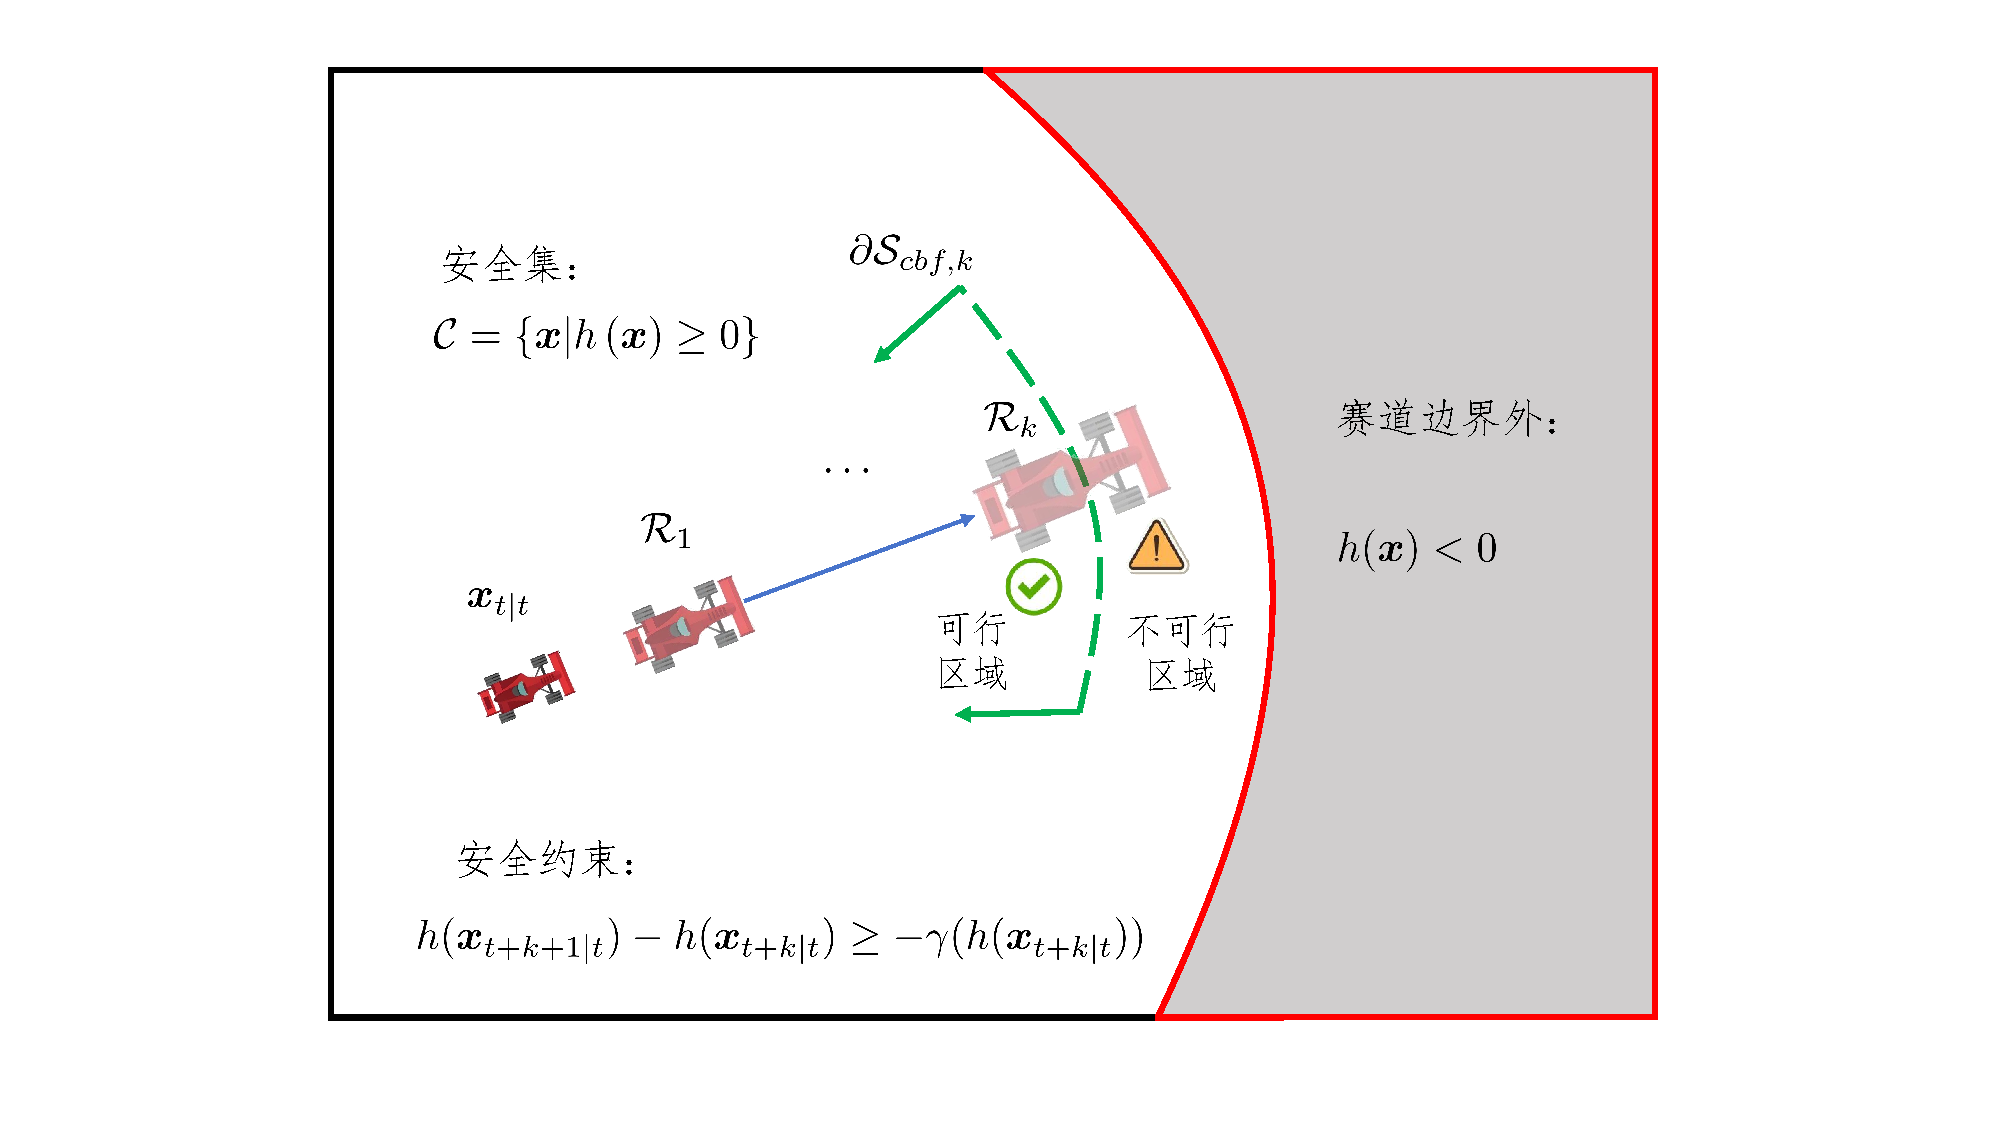
\includegraphics[width=0.65\linewidth]{figure/chapter2/cbf.pdf}
    \caption{控制障碍函数约束集示意图}
    \label{fig:cbf}
\end{figure}

控制障碍函数约束集的边界$\partial \mathcal{S}_{cbf,k}$可以被写作：
\begin{equation}
\begin{aligned}
    \partial \mathcal{S}_{cbf,k} = \{ \boldsymbol{x}_{t+k|t}\in\mathcal{X}| h(\boldsymbol{x}_{t+k|t})=(1-\gamma)h(\boldsymbol{x}_{t+k-1|t}) \}.
\end{aligned}
\end{equation}
$\gamma$取值越小，约束集$\mathcal{S}_{cbf,k}$的范围越小。在这种情况下，系统状态被要求在更严格的范围内，安全性更高，但$\mathcal{R}_k$与$\mathcal{S}_{cbf,k}$的交集可能为空，从而导致优化问题不可行。$\gamma$取值越大，约束集$\mathcal{S}_{cbf,k}$的范围越大，然而过大的$\gamma$值可能导致$\mathcal{R}_k$成为$\mathcal{S}_{cbf,k}$的子集，导致控制障碍约束无效。当$\gamma=1$时，约束集$\mathcal{S}_{cbf,k}$的边界$\partial \mathcal{S}_{cbf,k}$与安全集合的边界$\partial \mathcal{C}$重合，因此约束集$\mathcal{S}_{cbf,k}$是安全集$\mathcal{C}$的子集，因此当$\gamma<1$时，控制障碍函数比安全集更早起到约束作用，有效避免碰撞，从而提高系统的安全性。综上所述，通过合理选择$\gamma$的值，我们可以在保证优化问题可行性的前提下，实现安全竞速控制。

\subsection{基于控制障碍函数的模型预测轮廓控制}
为了将控制障碍函数应用于赛车在给定轨迹下的竞速控制，我们可以将其与模型预测轮廓控制（Model Predictive Contouring Control，简称MPCC）结合起来。MPCC是一种面向高速机动问题的模型预测控制方法，通过在优化问题中引入轮廓误差和滞后误差来实现沿着预定轨迹尽可能快速的跟踪\cite{liniger2015optimization, romero2022model, brito2019model}。下面我们将介绍MPCC的基本概念，并设计一种基于控制障碍函数的MPCC策略。

传统轨迹跟踪控制的思路是：首先预先规划一条参考轨迹，然后设计一个控制器来跟踪该轨迹。然而，这种方法在高速机动问题中可能会受到限制，因为竞速运动控制的本质是沿着预定轨迹尽可能快速地行驶，而不是简单地跟踪一个固定的轨迹；另外，预先规划的轨迹可能无法适应动态环境的变化，从而影响竞速性能。因此，MPCC的核心思想并不是最小化对时间参数轨迹的跟踪误差，而是最小化相对于赛道中心线的轮廓误差（Contouring Error）和滞后误差（Lag Error），同时最大化沿赛道方向的推进速度。

首先，设赛道中心线可以用弧长参数$s$来表示，赛道中心线上的点可以表示为$\boldsymbol{r}(s)=[X_c(s), Y_c(s)]^\top$，其中$X_c(s)$和$Y_c(s)$分别表示赛道中心线在全局坐标系下的横向和纵向位置，$s\in[0, L]$，$L$为赛道总长度。赛道的切线方向可以表示为$\boldsymbol{t}(s)=\frac{d \boldsymbol{r}(s)}{ds}=[X_c'(s), Y_c'(s)]^\top$。于是可以定义赛道切向角：$\phi_c(s) = \arctan2(Y_c'(s), X_c'(s))$，单位切向量为$\boldsymbol{e}_t(s)=[\cos{\phi_c(s)}, \sin{\phi_c(s)}]^\top$，单位法向量为$\boldsymbol{e}_n(s)=[-\sin{\phi_c(s)}, \cos{\phi_c(s)}]^\top$。

\begin{figure}[ht]
    \centering
    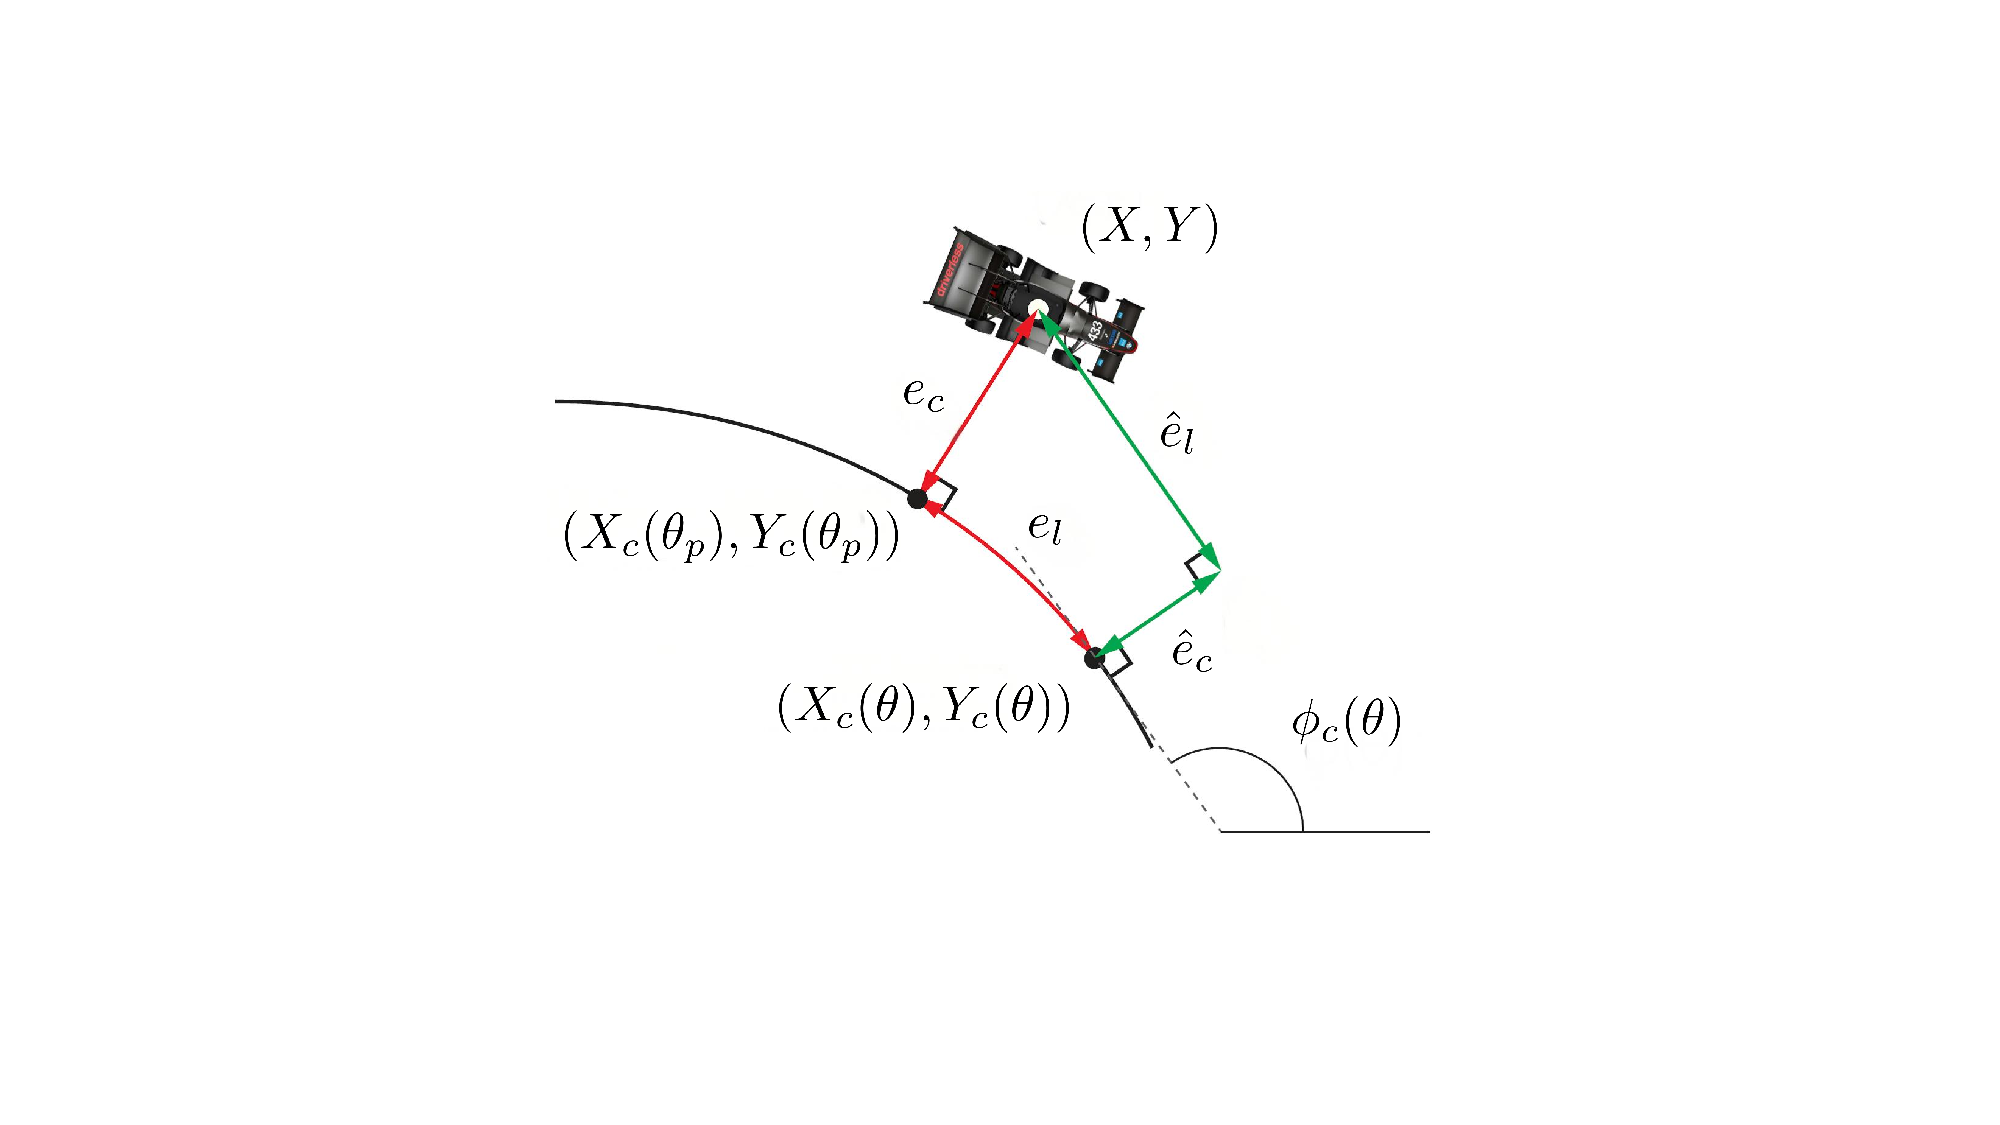
\includegraphics[width=0.5\linewidth]{figure/chapter2/contouring.pdf}
    \caption{轮廓误差和滞后误差示意图}
    \label{fig:contouring}
\end{figure}
为了能直接优化赛车在赛道上的进度，从而实现更高的竞速性能，MPCC引入了一个进度变量$\theta$，用于表示赛车在赛道上的路径进度，$\theta$的变化率$\dot{\theta}$表示赛车沿赛道方向的推进速度：$\dot{\theta} = v_{\theta}$。设赛车当前位置为$\boldsymbol{p}=[X, Y]^\top$，$\boldsymbol{p}$在赛道中心线上的投影为$\boldsymbol{r}(\theta_p)$，$\theta_p$表示赛车在赛道上的真实路径进度，通过最大化$\theta_p$即可实现高性能竞速。然而直接投影计算$\theta_p$会带来较大的计算负担，因此MPCC中通常将$\theta$作为一个独立的优化变量来近似表示赛车在赛道上的路径进度。为了使$\theta$能够准确地反映赛车在赛道上的位置，MPCC优化问题同时最小化用$\theta$估计的轮廓误差$\hat{e}_c$和滞后误差$\hat{e}_l$，如图\ref{fig:contouring}所示。定义位置偏差为$\boldsymbol{d}=\boldsymbol{p}-\boldsymbol{r}(\theta)$，轮廓误差$\hat{e}_c$表示车辆在赛道法向方向上的偏离程度，可以通过将位置偏差$\boldsymbol{d}$投影到单位法向量$\boldsymbol{e}_n(\theta)$上来计算得到：
\begin{equation}
\begin{aligned}
    \hat{e}_c = \boldsymbol{d}^\top \boldsymbol{e}_n(\theta) = -(X - X_c(\theta))\sin{\phi_c(\theta)} + (Y - Y_c(\theta))\cos{\phi_c(\theta)}.
\end{aligned}
\label{equ:contouring-error}
\end{equation}
滞后误差$\hat{e}_l$表示车辆在赛道切向方向上的偏离程度，可以通过将位置偏差$\boldsymbol{d}$投影到单位切向量$\boldsymbol{e}_t(\theta)$上来计算得到：
\begin{equation}
\begin{aligned}
    \hat{e}_l = \boldsymbol{d}^\top \boldsymbol{e}_t(\theta) = (X - X_c(\theta))\cos{\phi_c(\theta)} + (Y - Y_c(\theta))\sin{\phi_c(\theta)}.
\end{aligned}
\label{equ:lag-error}
\end{equation}
可以看出，用$\theta$估计的轮廓误差$\hat{e}_c$和滞后误差$\hat{e}_l$越小，$\theta$与赛车在赛道上的真实进度$\theta_p$越接近，越能真实反映赛车在赛道上的位置。

基于上述定义，我们重新改写状态变量和控制变量为：
\begin{equation}
\begin{aligned}
    \tilde{\boldsymbol{x}} = [X, Y, \phi, v_x, v_y, \omega, \theta]^\top, \ \tilde{\boldsymbol{u}} = [\delta, T, v_{\theta}]^\top.
\end{aligned}
\end{equation}
动力学方程为：
\begin{equation}
\begin{aligned}
    \tilde{\boldsymbol{x}}_{t+1} =\left[ \begin{matrix}
            \boldsymbol{x}_{t+1}  \\
            \theta_{t+1}  \\
        \end{matrix} \right] = \left[ \begin{matrix}
            f(\boldsymbol{x}_t, \boldsymbol{u}_t)  \\
            \theta_t + v_{\theta} \Delta t  \\
        \end{matrix} \right] = \tilde{f}(\tilde{\boldsymbol{x}}_t, \tilde{\boldsymbol{u}}_t),
\end{aligned}
\end{equation}
根据公式（\ref{equ:mpc-cbf}），我们可以构建一个基于控制障碍函数的MPCC优化问题（简称MPCC-CBF）如下：
{
    \allowdisplaybreaks
\begin{subequations}
\begin{align}
    \min_{\{\tilde{\boldsymbol{x}}, \tilde{\boldsymbol{u}}\}_{t:t+N-1|t}}\quad & \sum_{k=0}^{N-1} (q_c\hat{e}_{c,t+k|t}^2 + q_l\hat{e}_{l,t+k|t}^2 - q_{\theta} v_{\theta,t+k|t} + \tilde{\boldsymbol{u}}_{t+k|t}^\top R_{\tilde{\boldsymbol{u}}} \tilde{\boldsymbol{u}}_{t+k|t} + \notag\\
    & \qquad \Delta\tilde{\boldsymbol{u}}_{t+k|t}^\top R_{\Delta \tilde{\boldsymbol{u}}} \Delta\tilde{\boldsymbol{u}}_{t+k|t}) + q_c\hat{e}_{c,t+N|t}^2 + q_l\hat{e}_{l,t+N|t}^2, \\
    \text{s.t.}\quad &\forall k=0,\ldots,N-1: \notag \\
    & \tilde{\boldsymbol{x}}_{t+k+1|t} = \tilde{f}(\tilde{\boldsymbol{x}}_{t+k|t}, \tilde{\boldsymbol{u}}_{t+k|t}),\\
    & F_{y,f,t+k|t}^2 + F_{x,f,t+k|t}^2 \leq (\mu F_{z,f})^2,\\ \label{equ:friction1-constraint}
    & F_{y,r,t+k|t}^2 + F_{x,r,t+k|t}^2 \leq (\mu F_{z,r})^2,\\ \label{equ:friction2-constraint}
    & \tilde{\boldsymbol{u}}_{\text{min}} \leq \tilde{\boldsymbol{u}}_{t+k|t} \leq \tilde{\boldsymbol{u}}_{\text{max}},\\
    & \Delta\tilde{\boldsymbol{u}}_{\text{min}} \leq \Delta\tilde{\boldsymbol{u}}_{t+k|t} \leq \Delta\tilde{\boldsymbol{u}}_{\text{max}},\\
    & h(\tilde{\boldsymbol{x}}_{t+k+1|t}) \geq (1-\gamma)h(\tilde{\boldsymbol{x}}_{t+k|t}).\label{equ:mpcc-cbf-constraint}
\end{align}
\label{equ:mpcc-cbf}
\end{subequations}
}
其中，$q_c$、$q_l$和$q_{\theta}$分别是轮廓误差、滞后误差和推进速度的权重系数，$R_{\tilde{\boldsymbol{u}}}$和$R_{\Delta \tilde{\boldsymbol{u}}}$分别是控制输入和控制输入变化率的权重矩阵，$\Delta\tilde{\boldsymbol{u}}_{t+k|t} = \tilde{\boldsymbol{u}}_{t+k|t} - \tilde{\boldsymbol{u}}_{t+k-1|t}$，$\hat{e}_{c,t+k|t}$和$\hat{e}_{l,t+k|t}$分别由公式（\ref{equ:contouring-error}）和公式（\ref{equ:lag-error}）计算得到。公式（\ref{equ:friction1-constraint}）和公式（\ref{equ:friction2-constraint}）分别表示前轮和后轮的摩擦力约束，$F_{z,f}=\frac{lr}{lf+lr}mg$，$F_{z,r}=\frac{lf}{lf+lr}mg$为前轮和后轮的垂直载荷，前后轮驱动力$F_{x,f}$和$F_{x,r}$近似为平均分配。通过求解上述优化问题，我们可以获得一个控制输入序列$\tilde{\boldsymbol{u}}_{t:t+N-1|t}$，其中第一个控制输入$\tilde{\boldsymbol{u}}_{t|t}$被应用于系统，以实现基于控制障碍函数的MPCC策略。

控制障碍函数约束（\ref{equ:mpcc-cbf-constraint}）确保了在整个预测时域内，系统状态始终保持在安全集合内，从而保证了赛车的安全性。对于已知赛道环境的安全竞速问题，控制障碍函数主要分为两种：（1）防止赛车与赛道边界相撞；（2）防止赛车与其他车辆相撞。第一种障碍函数设计为如下形式：
\begin{equation}
\begin{aligned}
    h_1(\tilde{\boldsymbol{x}}_{t+k|t})=1-\frac{\hat{e}_{c,t+k|t}^2}{(l_{max}-l_2)^2},
\end{aligned}
\end{equation}
其中，车辆可视为一个矩形，长为$2l_1$，宽为$2l_2$，赛道最大可行驶宽度为$2 l_{max}$。第二种障碍函数与第$j$个其他车辆有关：
\begin{equation}
\begin{aligned}
h_2^j(\tilde{\boldsymbol{x}}_{t+k|t})=\frac{(\theta_{t+k|t}-\theta^j_{t+k|t})^2}{(2l_1)^2}+\frac{(\hat{e}_{c,t+k|t}-\hat{e}_{c,t+k|t}^j)^2}{(2l_2)^2}-1,
\end{aligned}
\end{equation}
其中，$j=1,\ldots,N_v$，$N_v$为赛道上其他车辆的数量，$\theta^j_{t+k|t}$和$\hat{e}_{c,t+k|t}^j$分别表示第$j$个车辆在预测时刻$t+k|t$的进度和轮廓误差。
\newpage
\section{仿真与实车实验}
在仿真环境中，所有车辆的运动状态和控制输入都可以被精确测量和控制。车辆的长度为0.4m，宽度为0.25m。赛道宽度设为2m。假设仿真环境中所有车辆的位置和姿态信息都已知，且相互之间不存在交互和博弈行为。公式（\ref{equ:mpcc-cbf}）是一个典型的非线性优化问题，本文中使用了Python中的Casadi\cite{andersson2018casadi}作为符号函数，以及IPOPT\cite{biegler2009large}作为非线性优化求解器来求解该优化问题。优化问题在一台CPU为Intel i9-12900H的电脑上运行。为了加速求解过程，我们使用了MPCC-CBF优化问题的初始解生成方法，即首先求解一个不包含控制障碍函数约束的MPCC优化问题，得到一个初始解，然后将该初始解作为包含控制障碍函数约束的MPCC优化问题的初始解来加速求解过程。表\ref{tab:mpcc-params}展示了MPCC-CBF控制器的参数设置示例。另外，每一次迭代优化前使用前一次迭代的优化结果作为初始解来加速求解过程。
\begin{table}[h]
    \caption{\label{tab:mpcc-params}MPCC-CBF控制器参数}
    \renewcommand\arraystretch{1.25}
    \setlength{\tabcolsep}{20pt}{
    \begin{tabular}{cc||cc}
    \toprule[2pt]
        参数    & 大小 & 参数  & 大小 \\ \midrule[1pt]
        $q_c$     & $0.1$    & $\tilde{\boldsymbol{u}}_{\text{min}}$ & $[-1, -0.45, -0.1]^\top$     \\
        $q_l$     & $1000.0$    & $\tilde{\boldsymbol{u}}_{\text{max}}$ & $[1, 0.45, 15.0]^\top$     \\
        $q_{\theta}$     & $5.0$   & $\Delta\tilde{\boldsymbol{u}}_{\text{min}}$ & $[-0.5, -0.15, -0.5]^\top$     \\
        $R_{\tilde{\boldsymbol{u}}}$ & $diag(1e^{-3}, 5e^{-2}, 1e^{-3})$     & $\Delta\tilde{\boldsymbol{u}}_{\text{max}}$ & $[0.5, 0.15, 0.5]^\top$     \\
        $R_{\Delta \tilde{\boldsymbol{u}}}$ & $diag(1e^{-3}, 5e^{-2}, 1e^{-3})$     &   $N$    &  $40$        \\
        $\gamma$ & $0.5$ & $\Delta t$ & $0.05$ \\ \bottomrule[2pt]
    \end{tabular}}
\end{table}
\subsection{静态避障实验与安全性分析}
首先，我们在一个静态环境中验证了MPCC-CBF控制器的性能。仿真环境中只有一辆赛车，其他车辆静止不动。我们将赛车初始化在赛道中心线附近，并让其沿着赛道进行竞速控制。图\ref{fig:mpcc-cbf-static}展示了MPCC-CBF在静态环境下的运动轨迹，图\ref{fig:mpcc-cbf-static-control}展示了对应的控制输入。可以看出，赛车能够沿着赛道中心线进行竞速控制，同时保持安全距离，避免与赛道边界发生碰撞；控制输入的变化也比较平滑，没有出现过大的控制输入变化；滞后误差较小，控制器能准确估计赛车在赛道上的位置，从而实现高性能的竞速控制。在拐入弯道时，赛车采用入弯前外侧、入弯内侧、出弯外侧的行驶策略来提高过弯性能，同时保持安全距离，避免与赛道边界发生碰撞。
\begin{figure}[H]
    \centering
    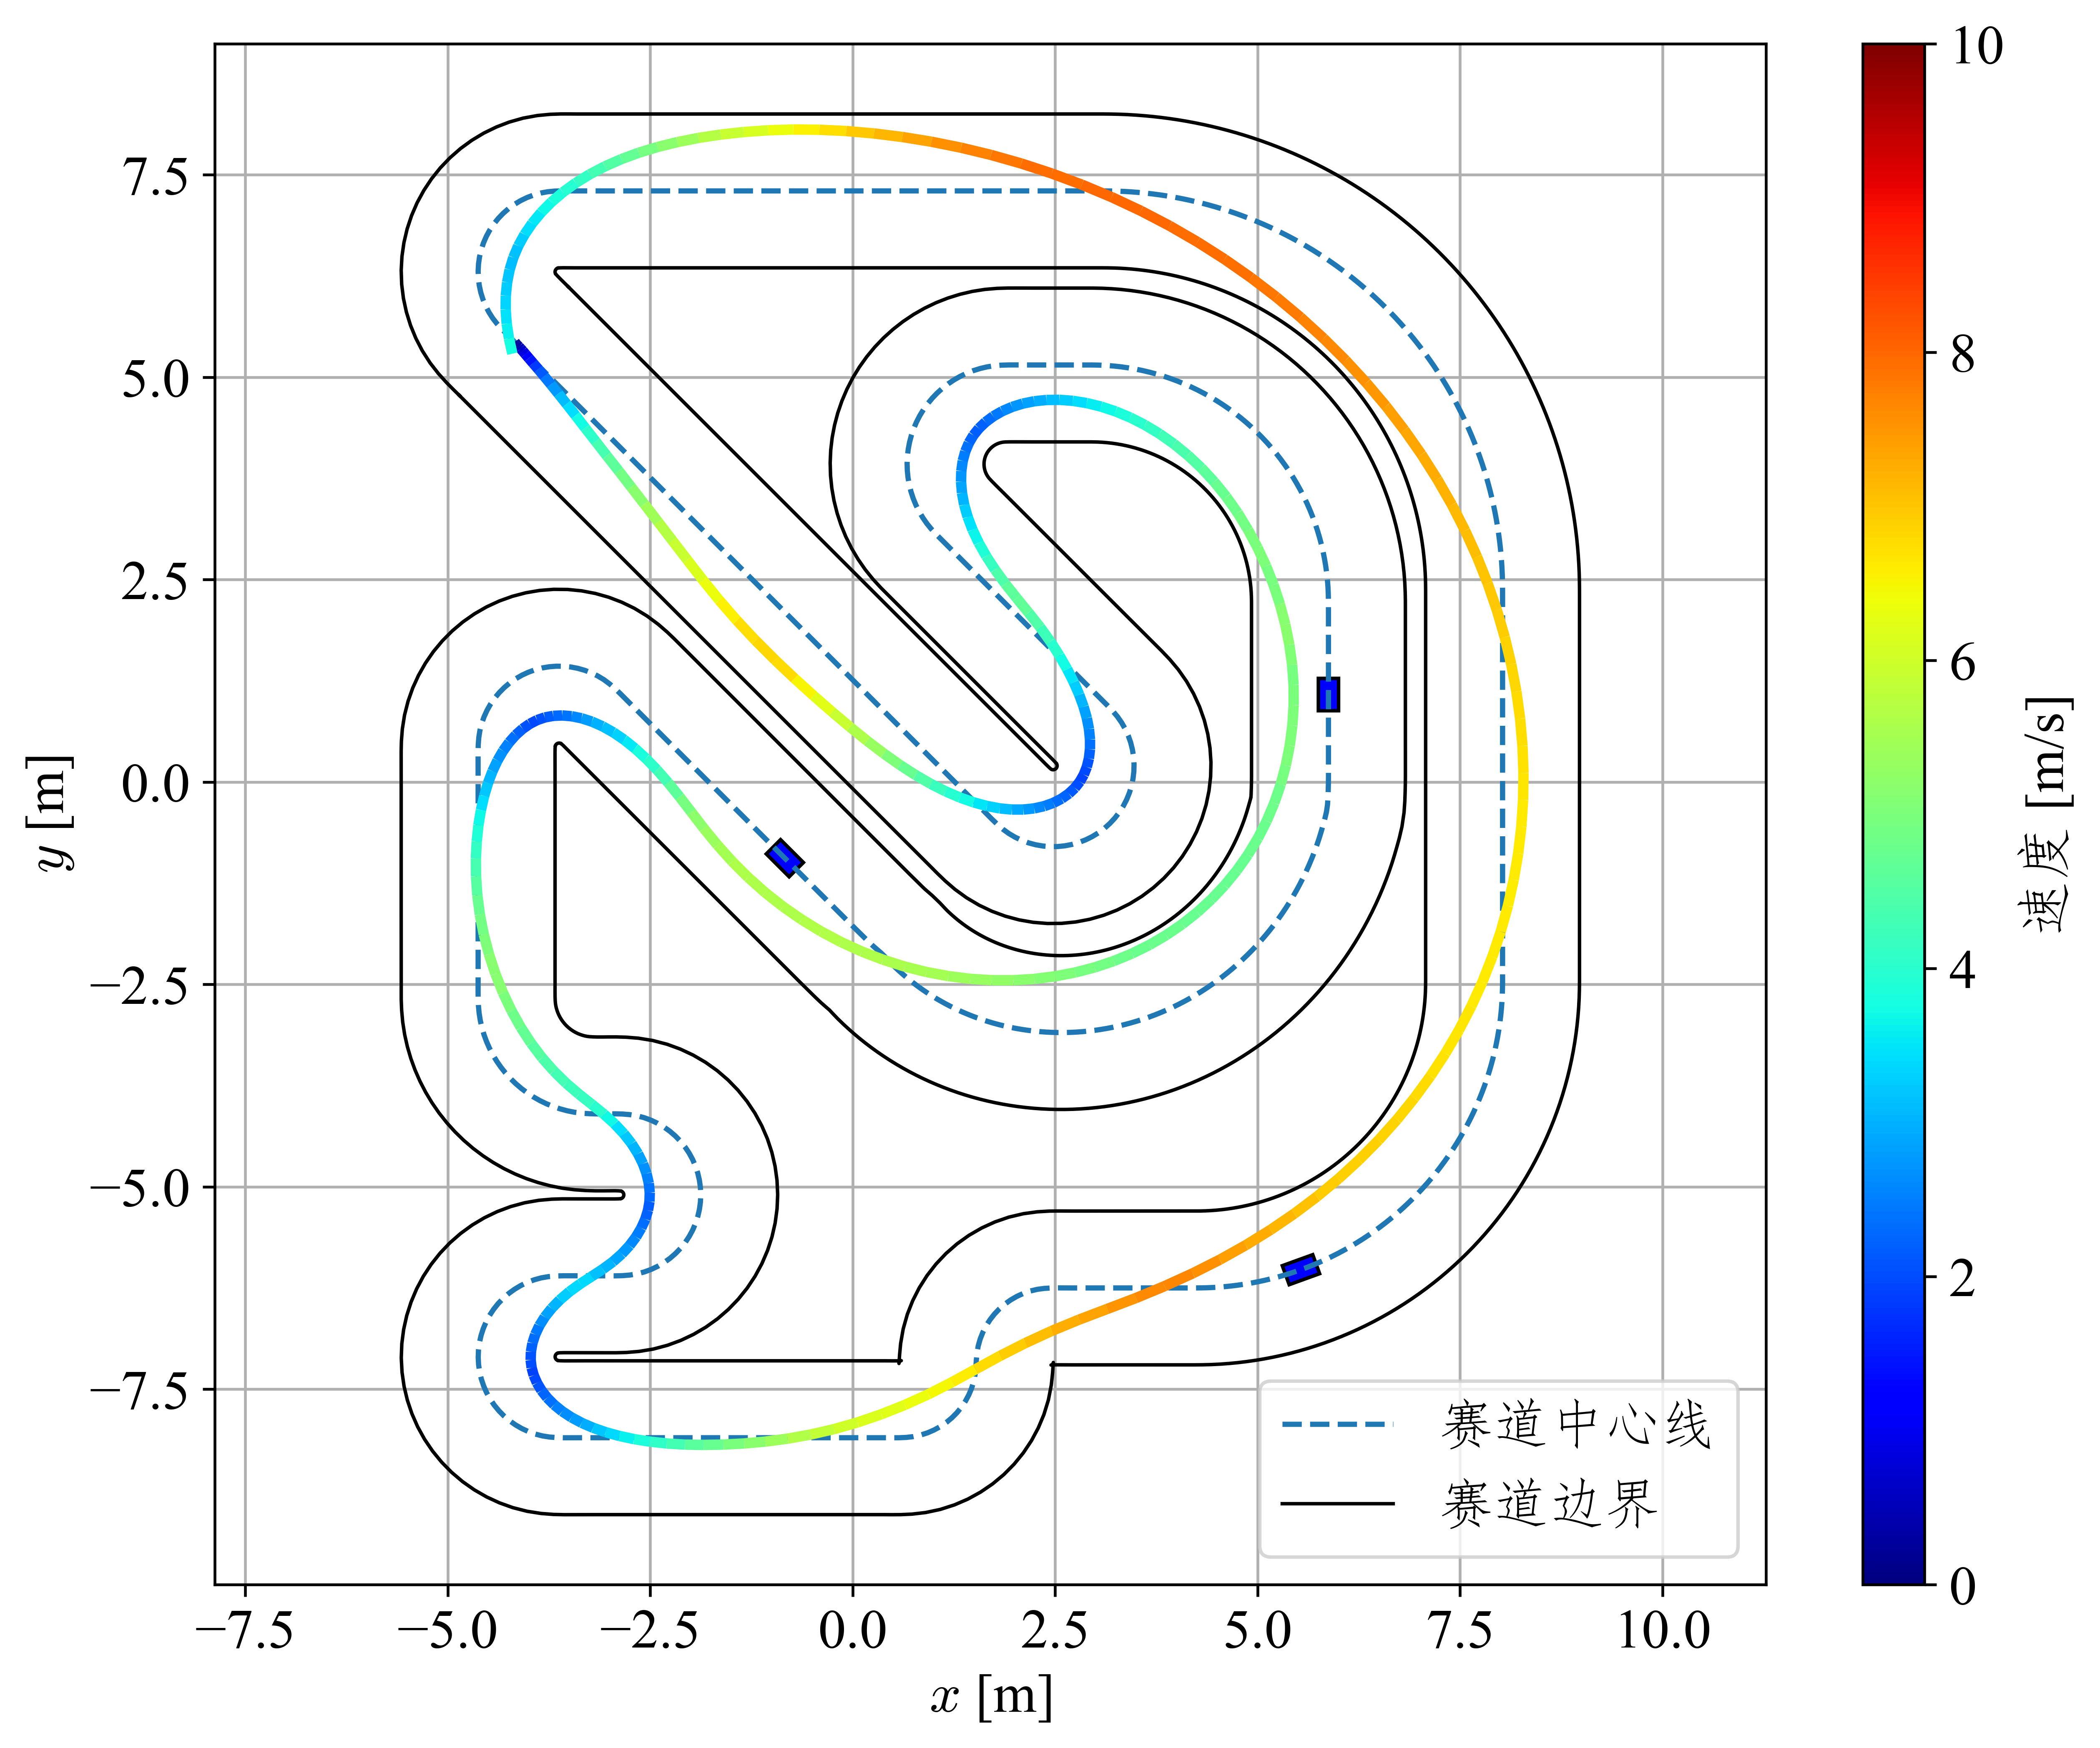
\includegraphics[width=0.6\linewidth]{figure/chapter2/mpcc_cbf_gamma0.5_static_trajectory.png}
    \caption{MPCC-CBF控制器在静态环境下的运动轨迹}
    \label{fig:mpcc-cbf-static}
\end{figure}
\begin{figure}[H]
    \centering
    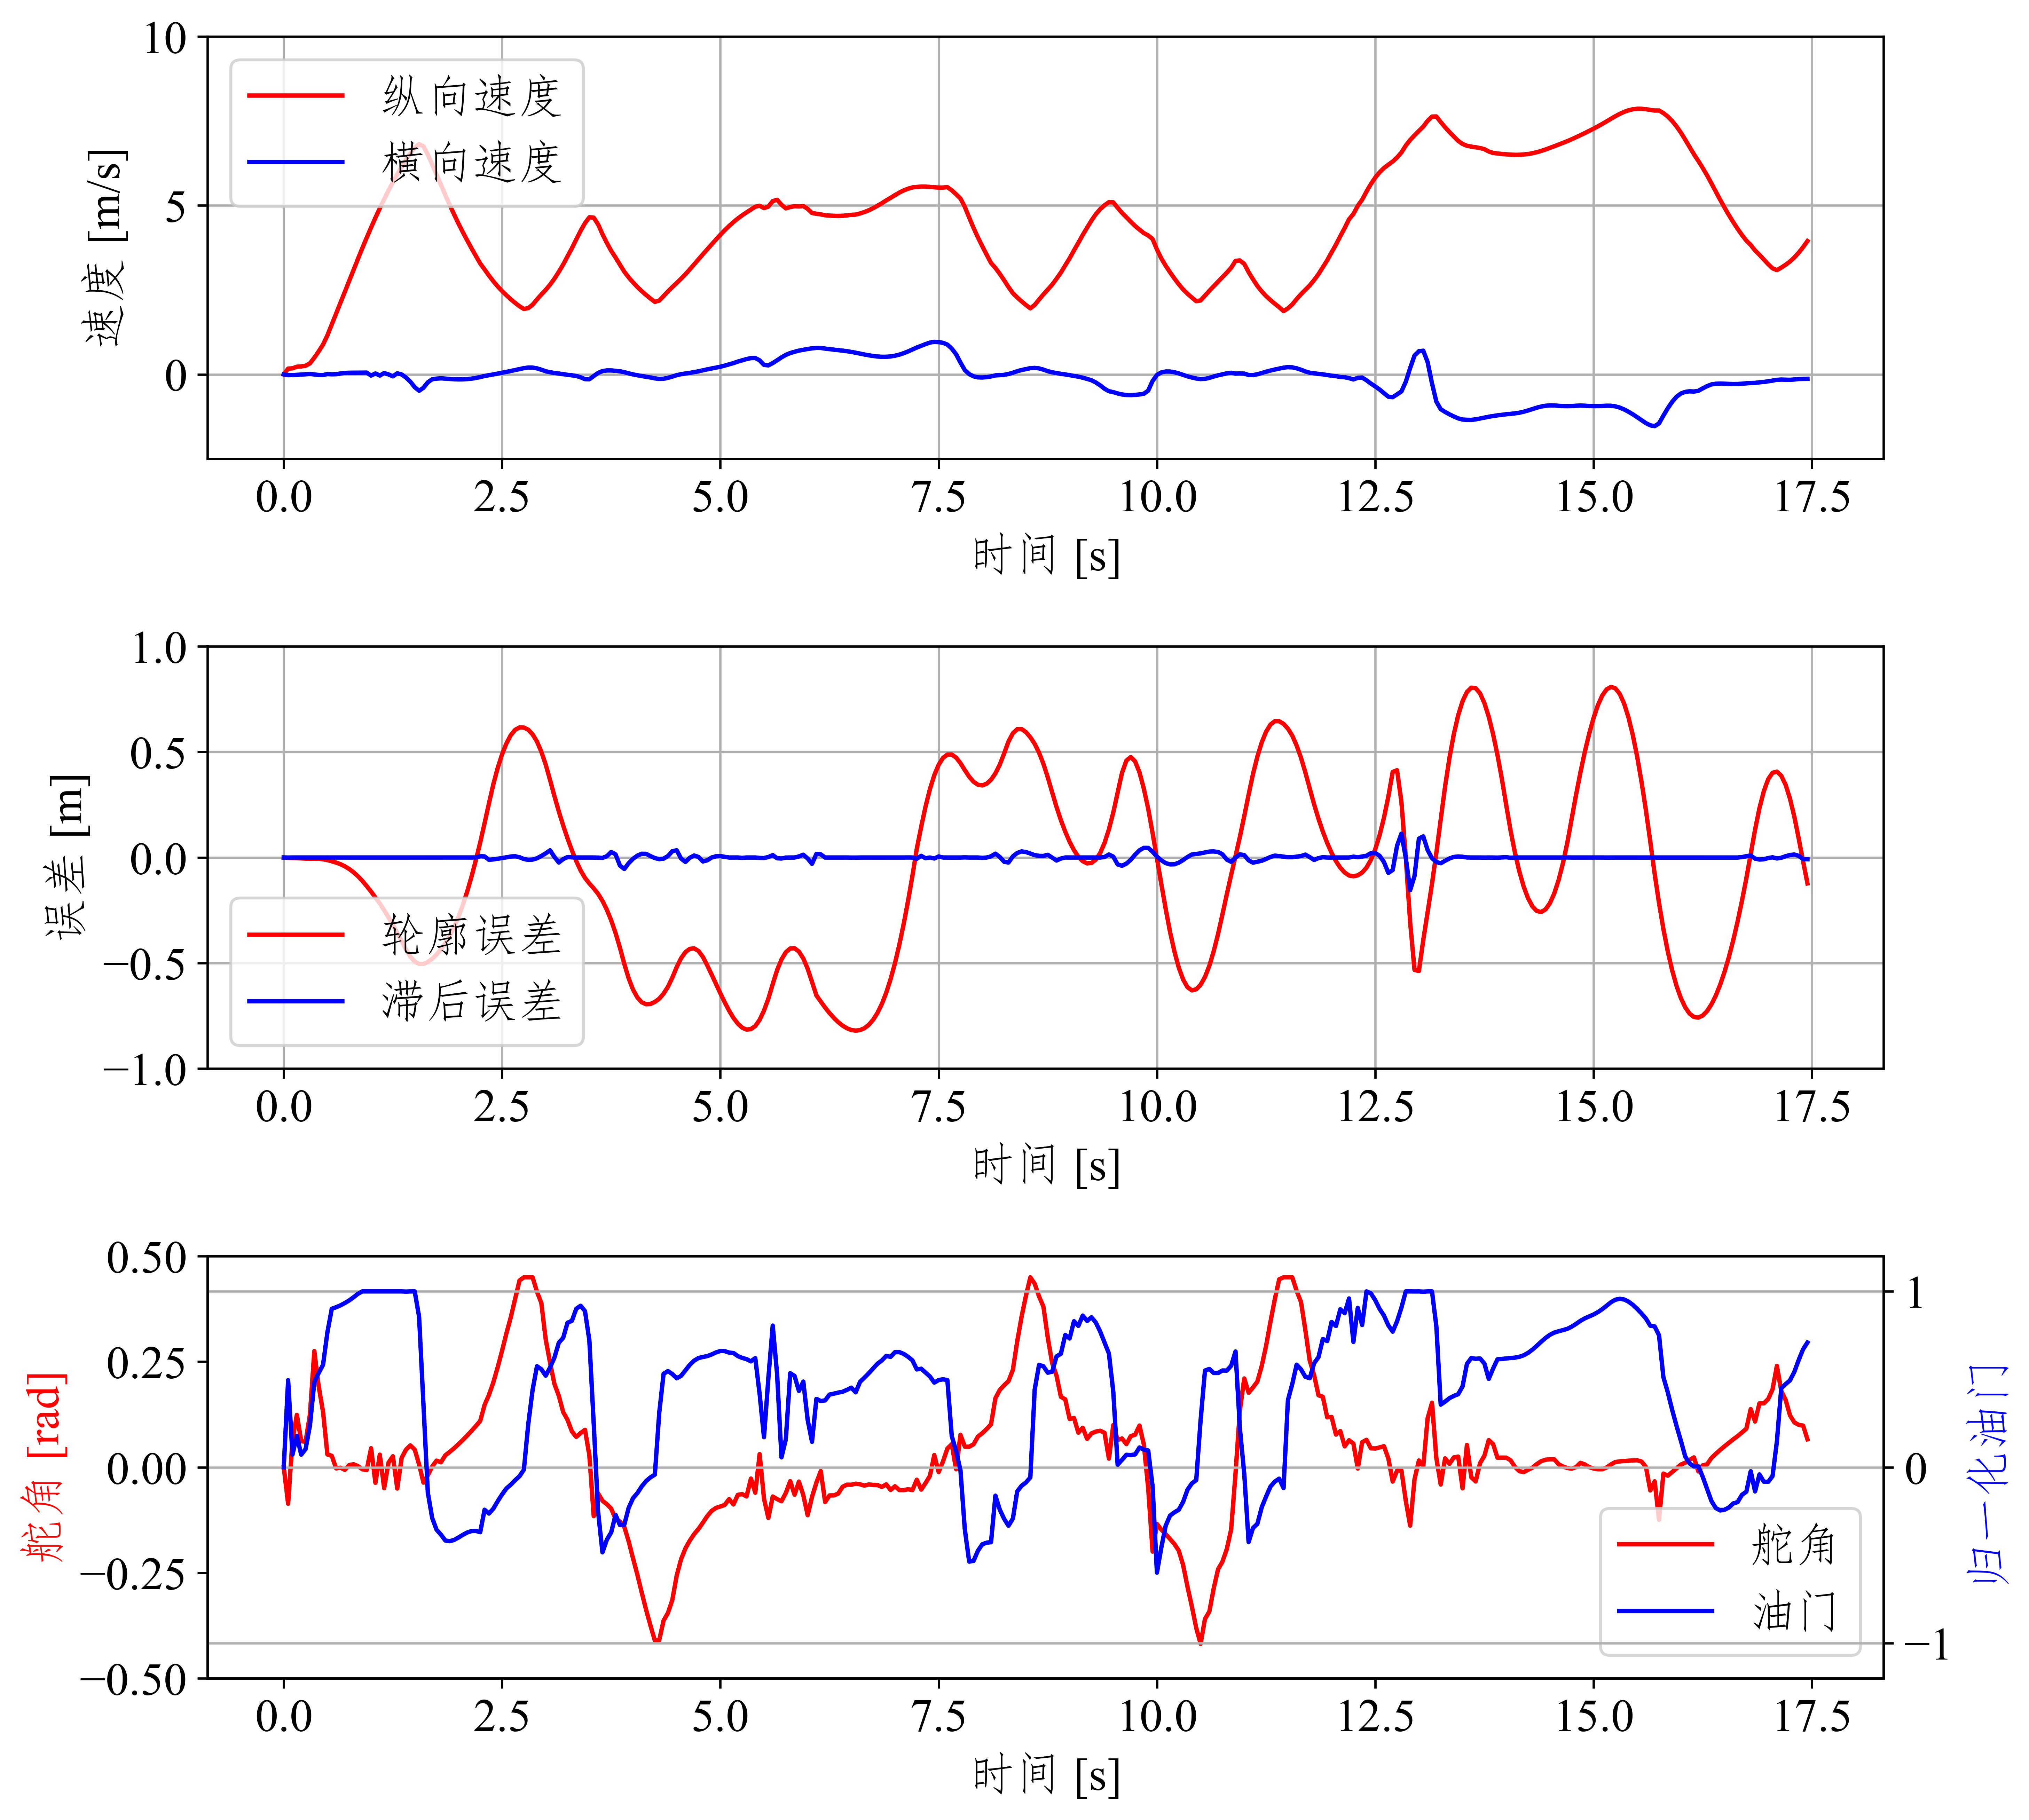
\includegraphics[width=0.75\linewidth]{figure/chapter2/mpcc_cbf_gamma0.5_control_inputs.png}
    \caption{MPCC-CBF控制器在静态环境下的控制输入变化曲线}
    \label{fig:mpcc-cbf-static-control}
\end{figure}

\newpage
另外，我们通过实验比较了不同$\gamma$值下MPCC-CBF控制器的性能。表\ref{tab:different-cbf-results}展示了不同$\gamma$值下MPCC-CBF控制器在单圈时间、距障碍物最小距离、平均速度和最大速度等指标上的比较结果。图\ref{fig:different-cbf-trajectory}展示了不同$\gamma$值下的运动轨迹。其中，$\gamma=1$时，控制障碍函数失效，退化为普通的MPCC控制器。可以看出，随着$\gamma$值的增加，赛车的单圈时间逐渐减少，平均速度和最大速度逐渐增加，但距障碍物的最小距离逐渐减小。这表明较大的$\gamma$值能够提高赛车的竞速性能，但可能会降低安全性。
\begin{table}[h]
    \caption{\label{tab:different-cbf-results}不同$\gamma$值下MPCC-CBF控制器的性能比较}
    \renewcommand\arraystretch{1.25}
    \setlength{\tabcolsep}{8pt}{
    \begin{tabular}{ccccc}
    \toprule[2pt]
        $\gamma$取值 & 单圈时间[s] & 距障碍物最小距离[m] & 平均速度[m/s] & 最大速度[m/s] \\ \midrule[1pt]
        $0.1$     & $21.70$  & $0.755$ & $3.78$ & $7.80$ \\
        $0.3$     & $18.10$  & $0.599$ & $4.45$ & $7.83$ \\
        $0.5$     & $17.45$  & $0.447$ & $4.46$ & $7.98$ \\
        $0.7$     & $17.40$  & $0.287$ & $4.50$ & $7.99$ \\
        $1.0$     & $17.40$  & $0.248$ & $4.47$ & $8.01$ \\ \bottomrule[2pt]
    \end{tabular}}
\end{table}
\begin{figure}[ht]
\centering
\subfloat[$\gamma=0.1$]{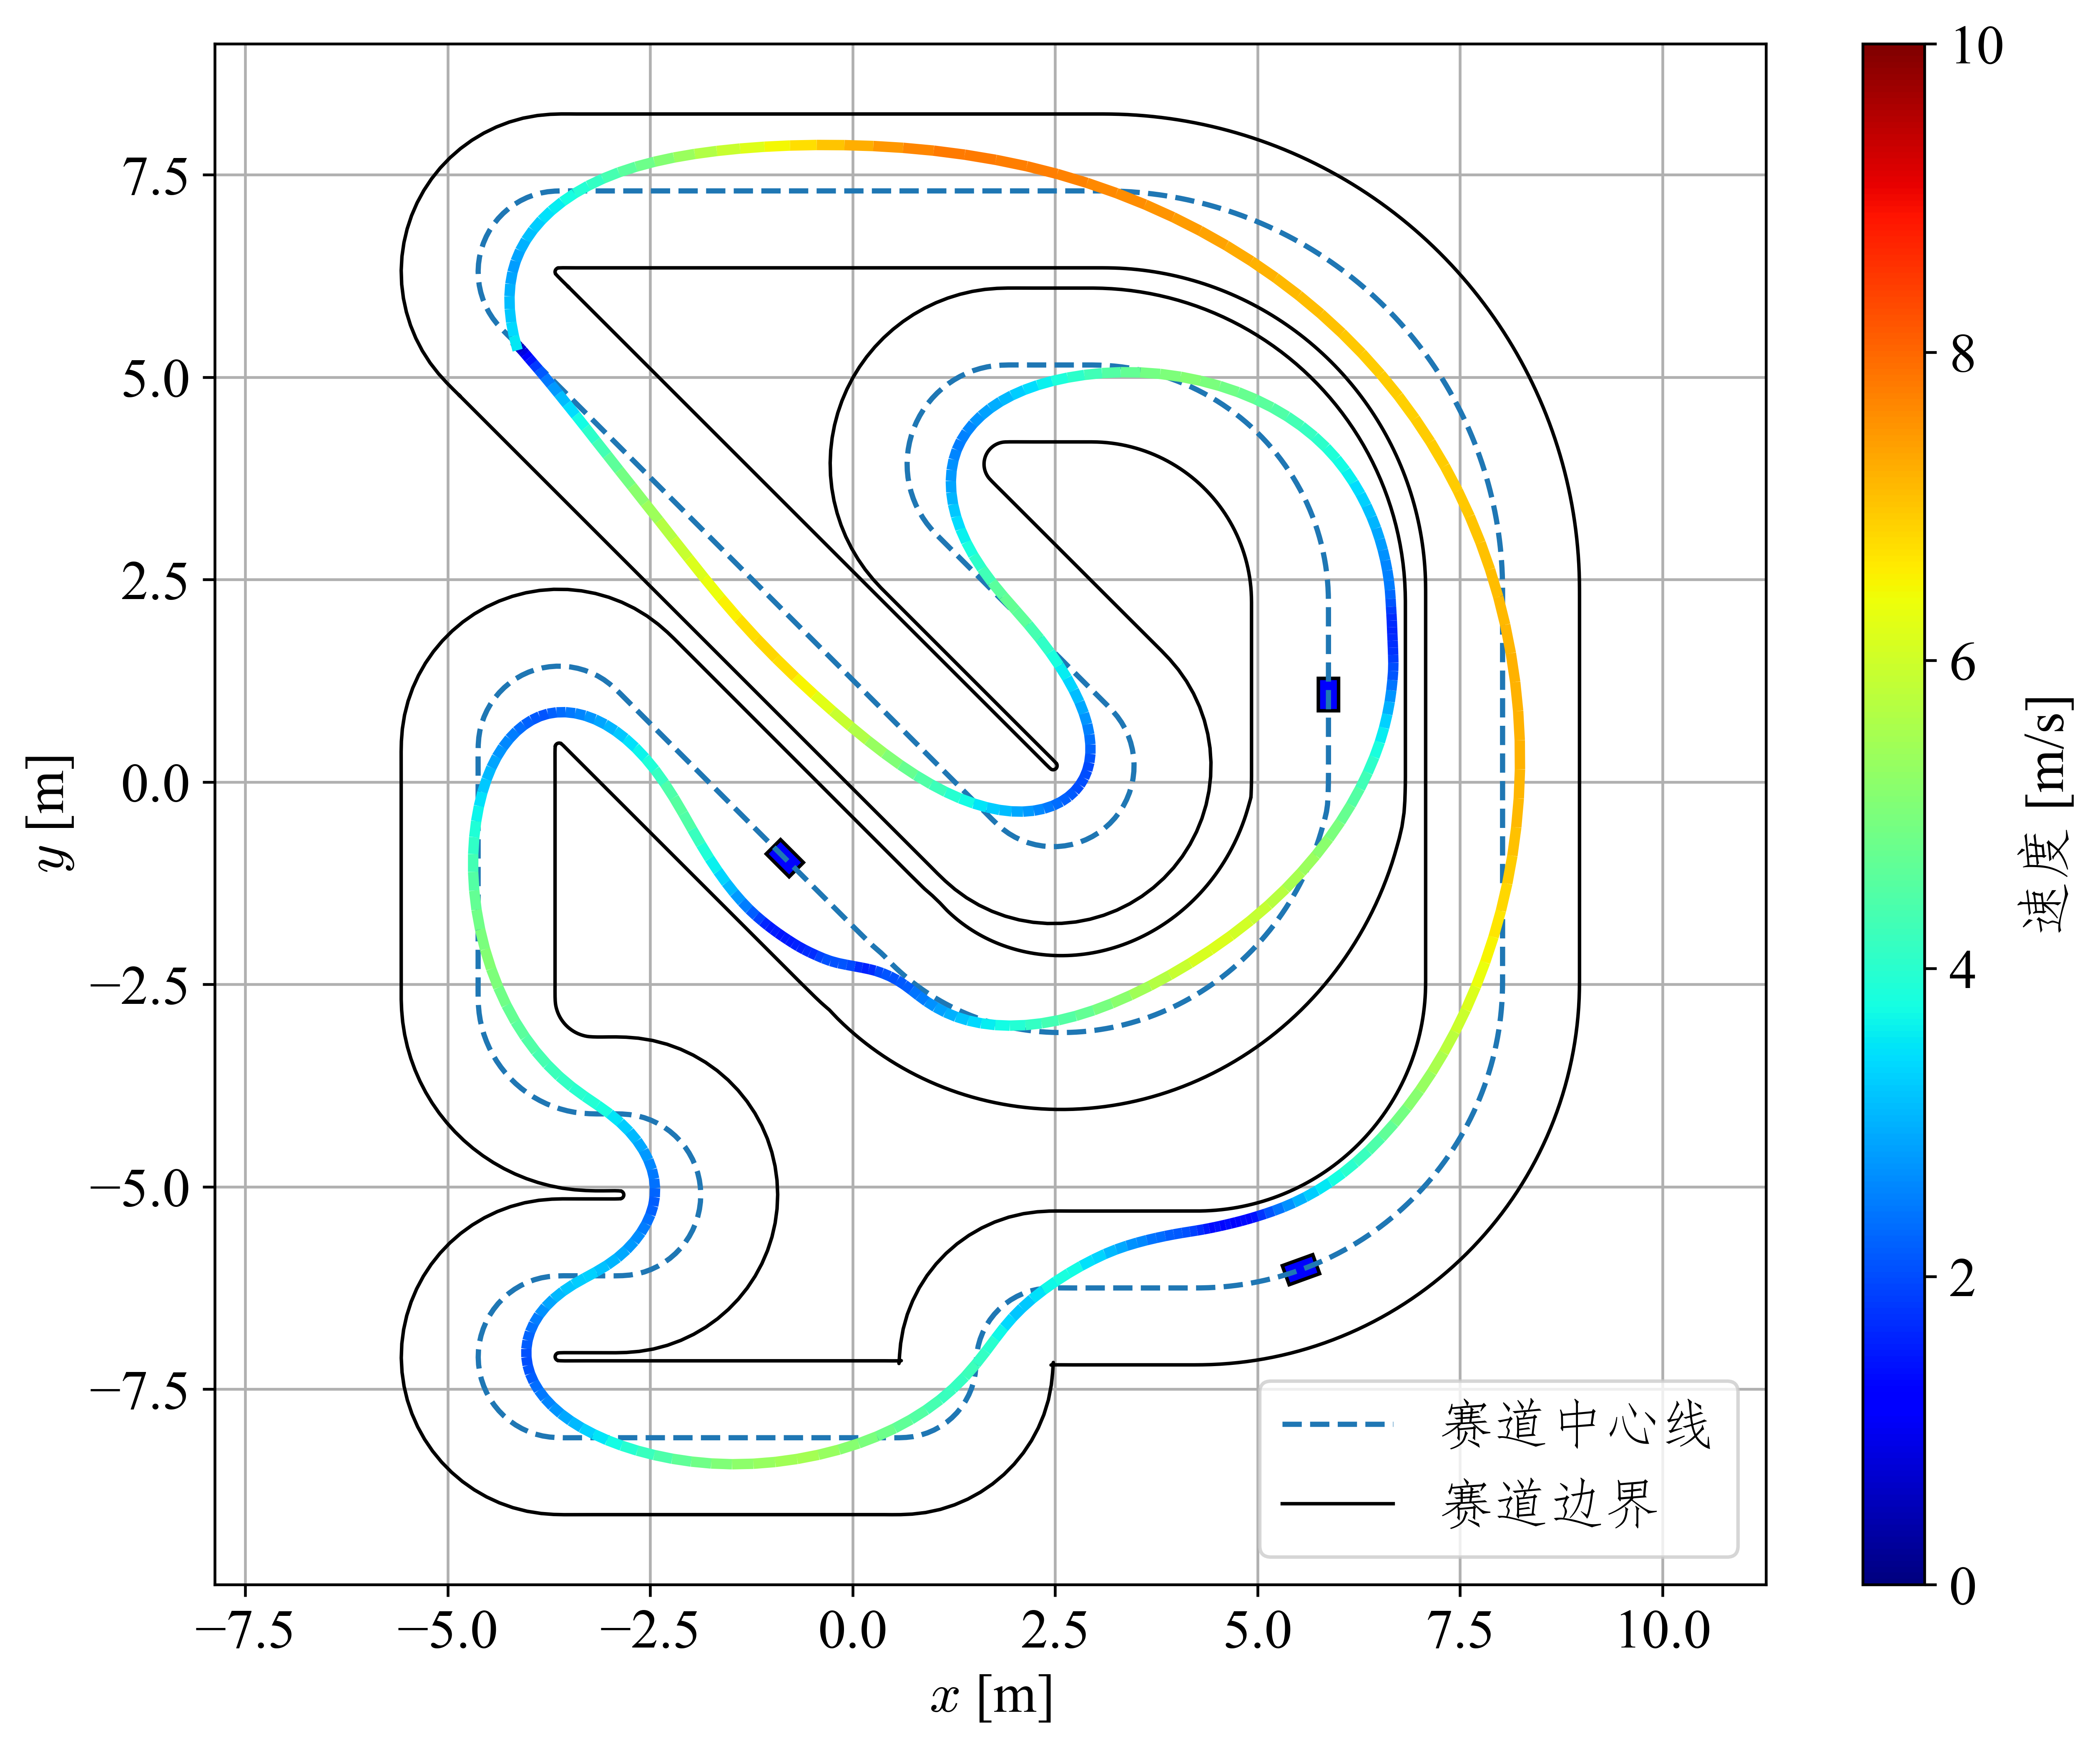
\includegraphics[width=0.33\linewidth]{figure/chapter2/mpcc_cbf_gamma0.1_static_trajectory.png}}
\subfloat[$\gamma=0.3$]{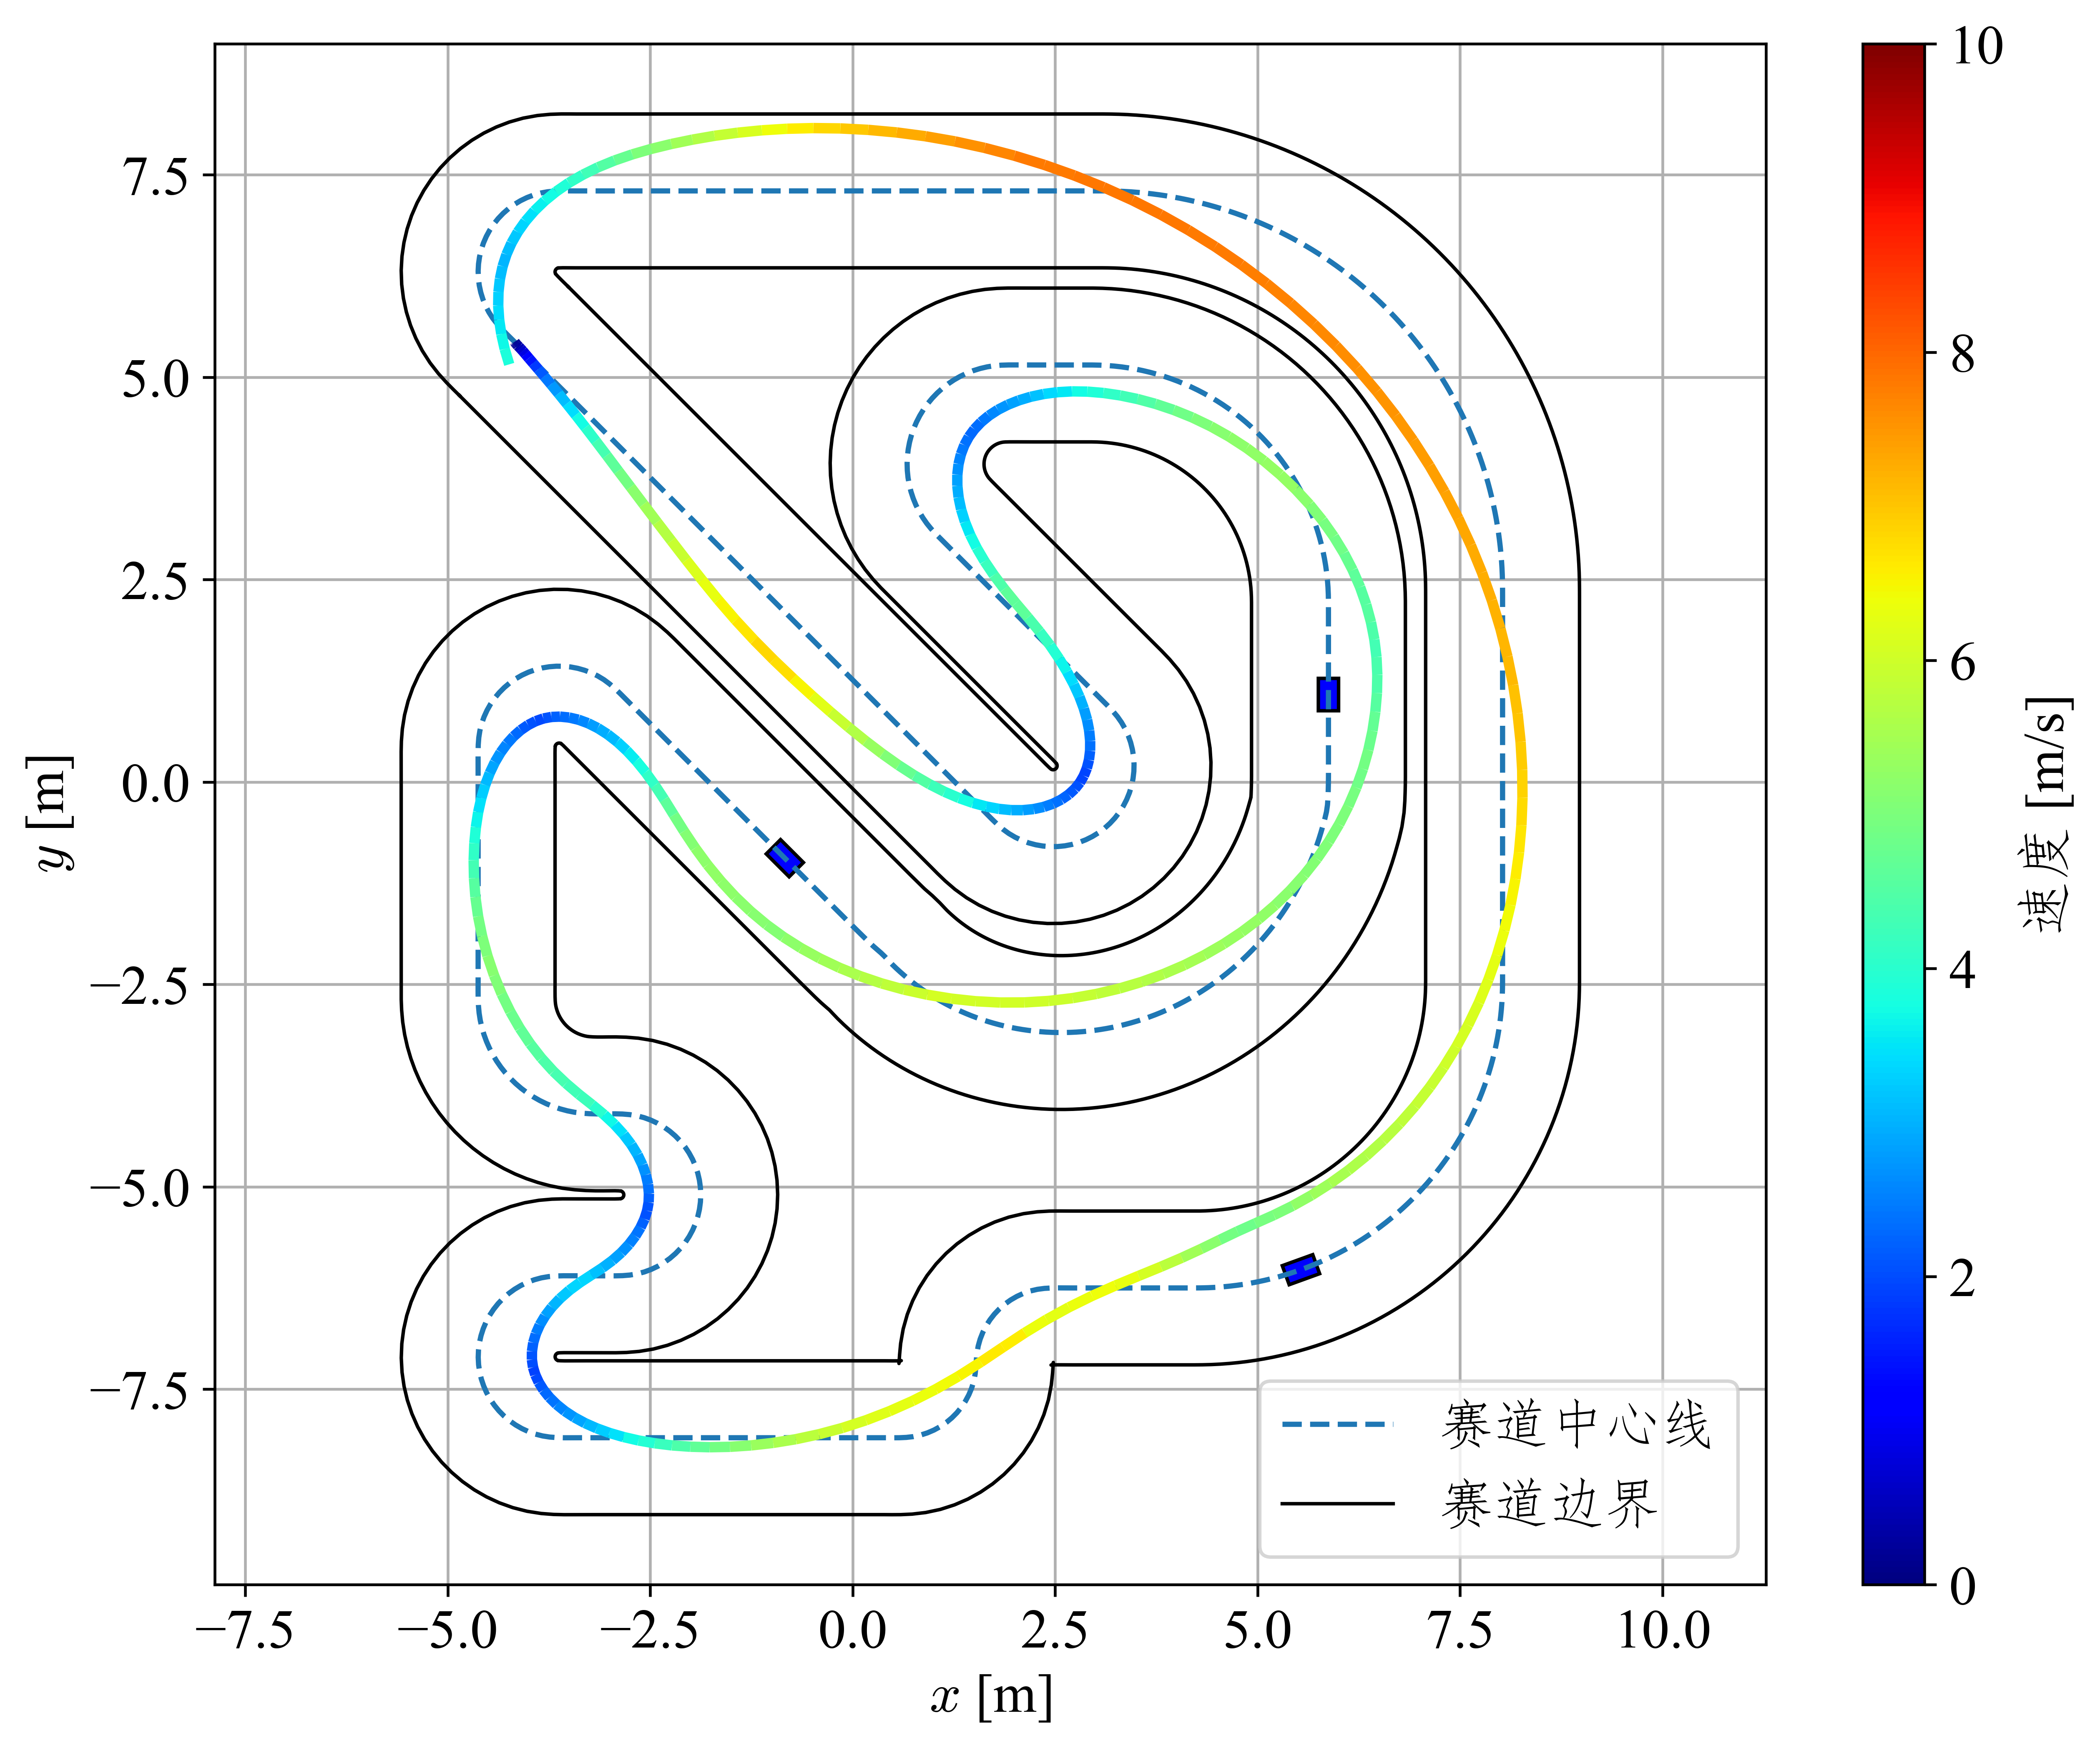
\includegraphics[width=0.33\linewidth]{figure/chapter2/mpcc_cbf_gamma0.3_static_trajectory.png}}
\subfloat[$\gamma=0.5$]{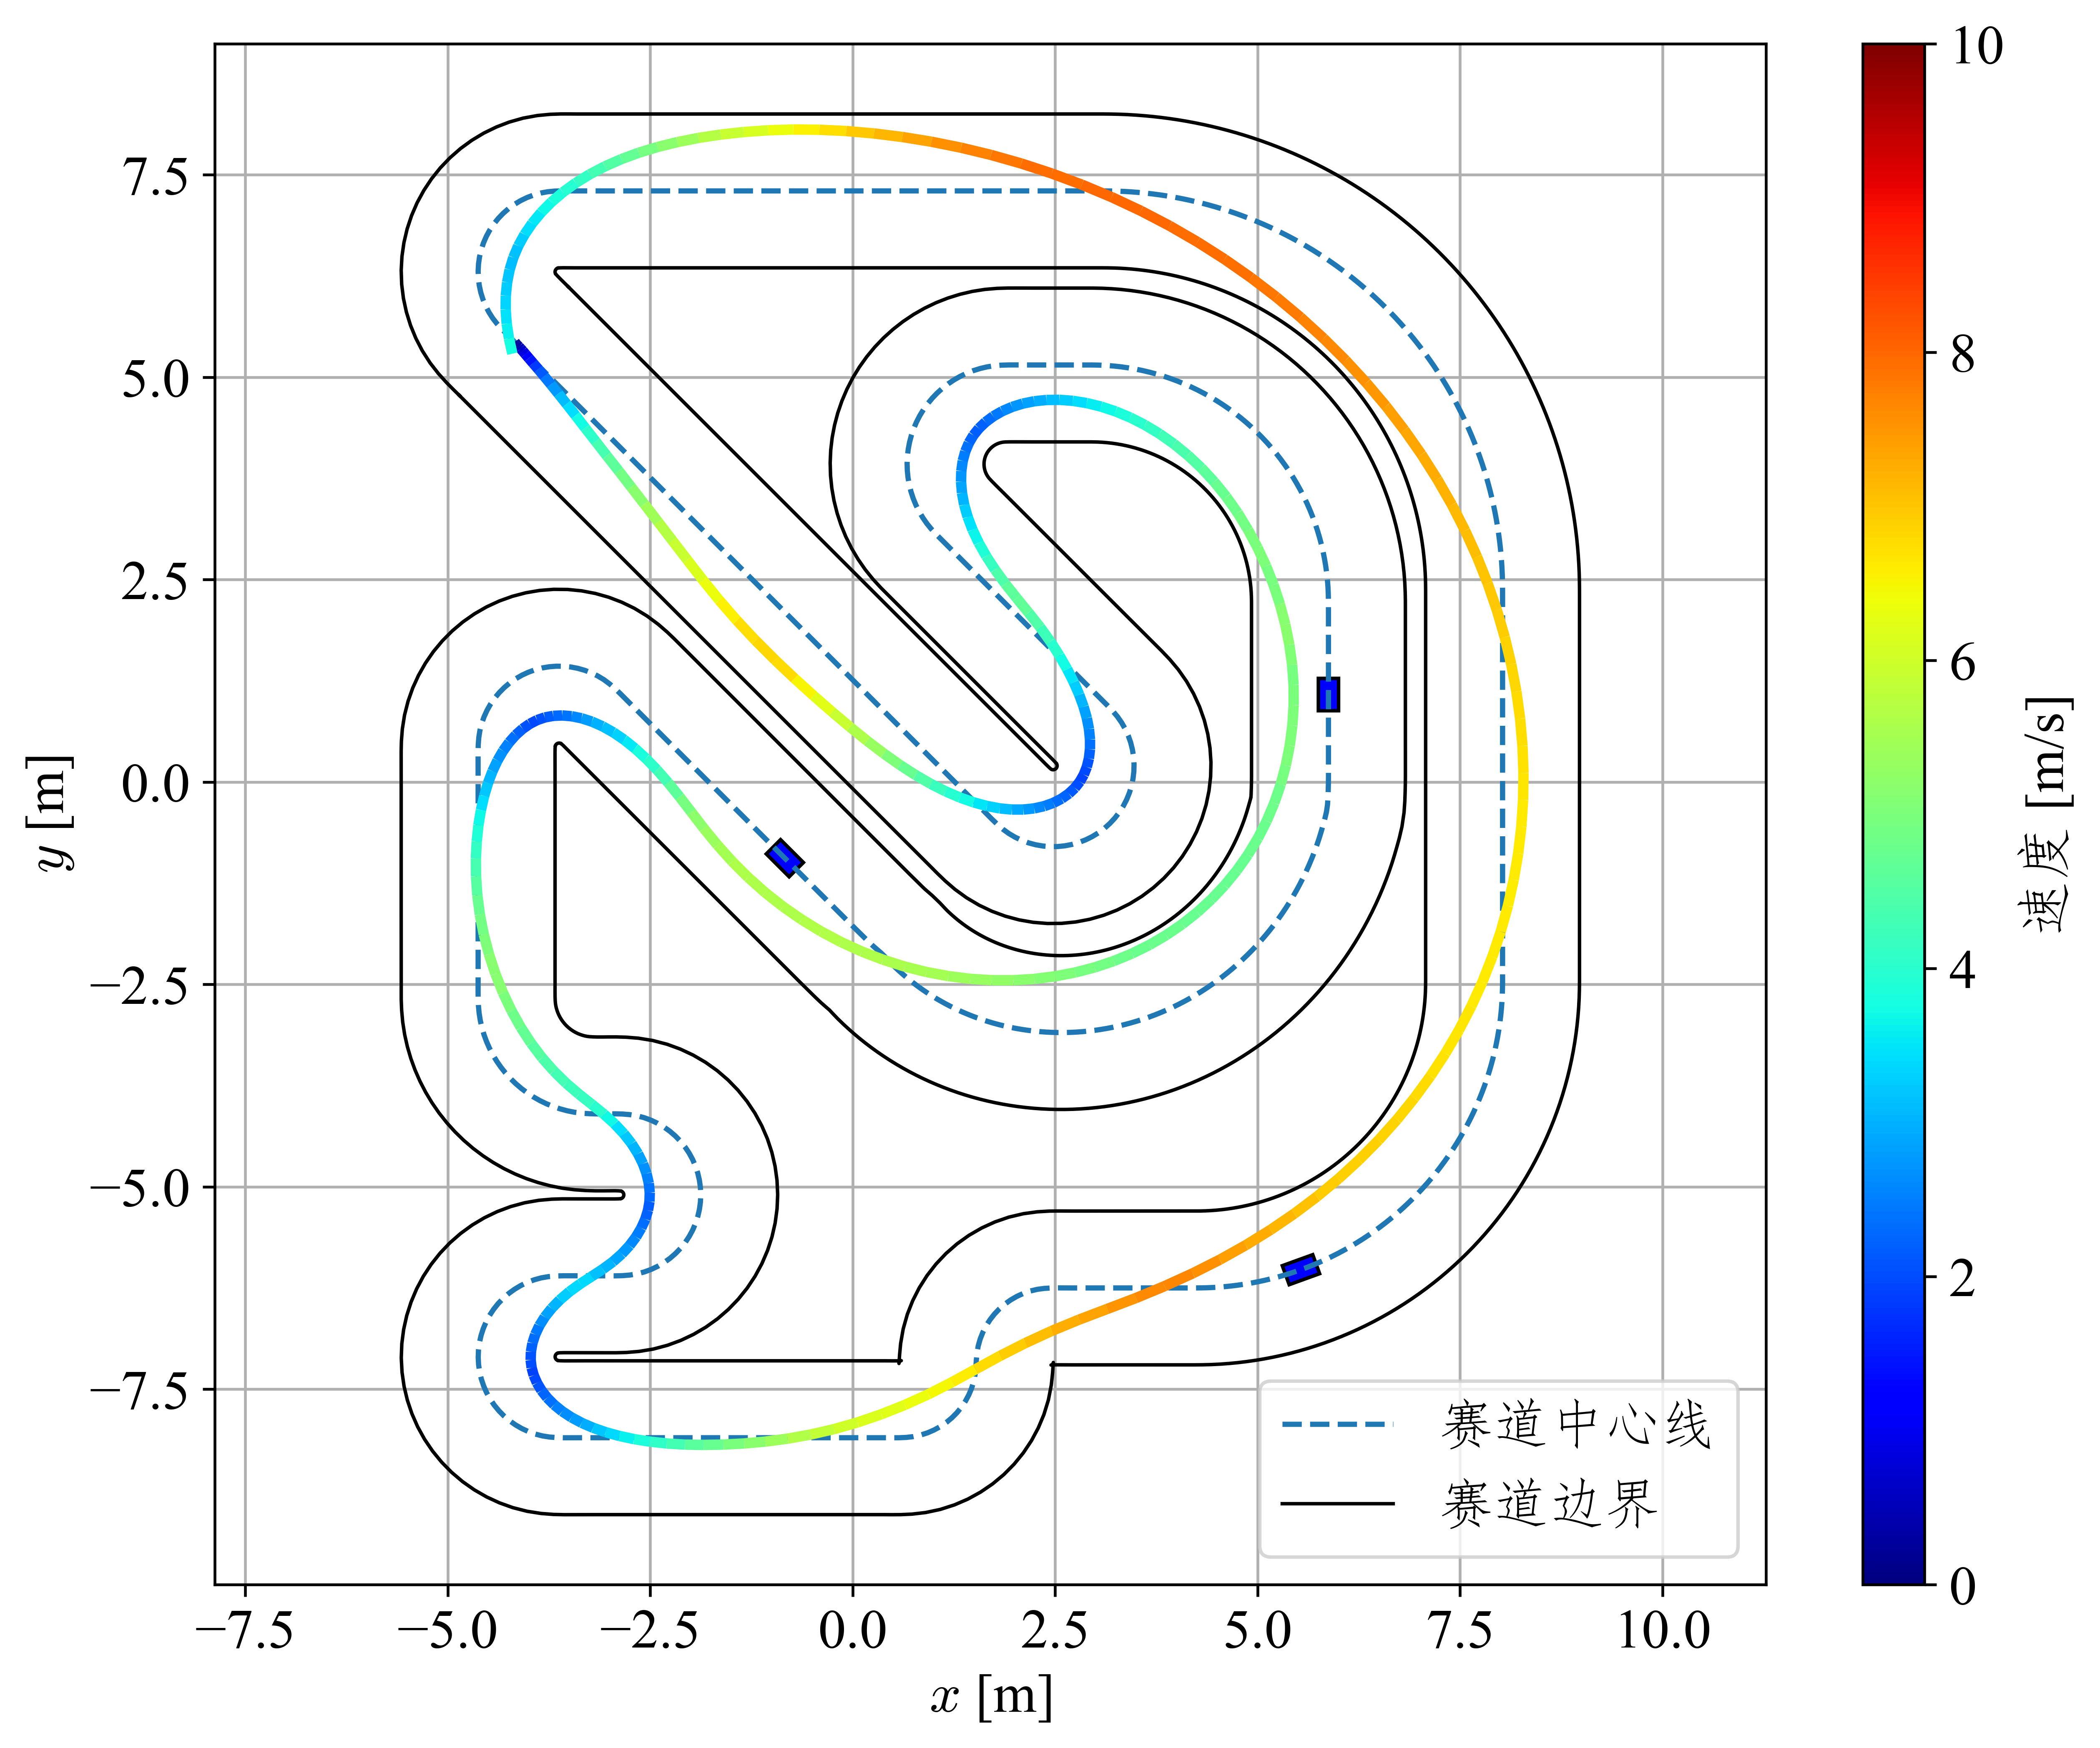
\includegraphics[width=0.33\linewidth]{figure/chapter2/mpcc_cbf_gamma0.5_static_trajectory.png}}

\subfloat[$\gamma=0.7$]{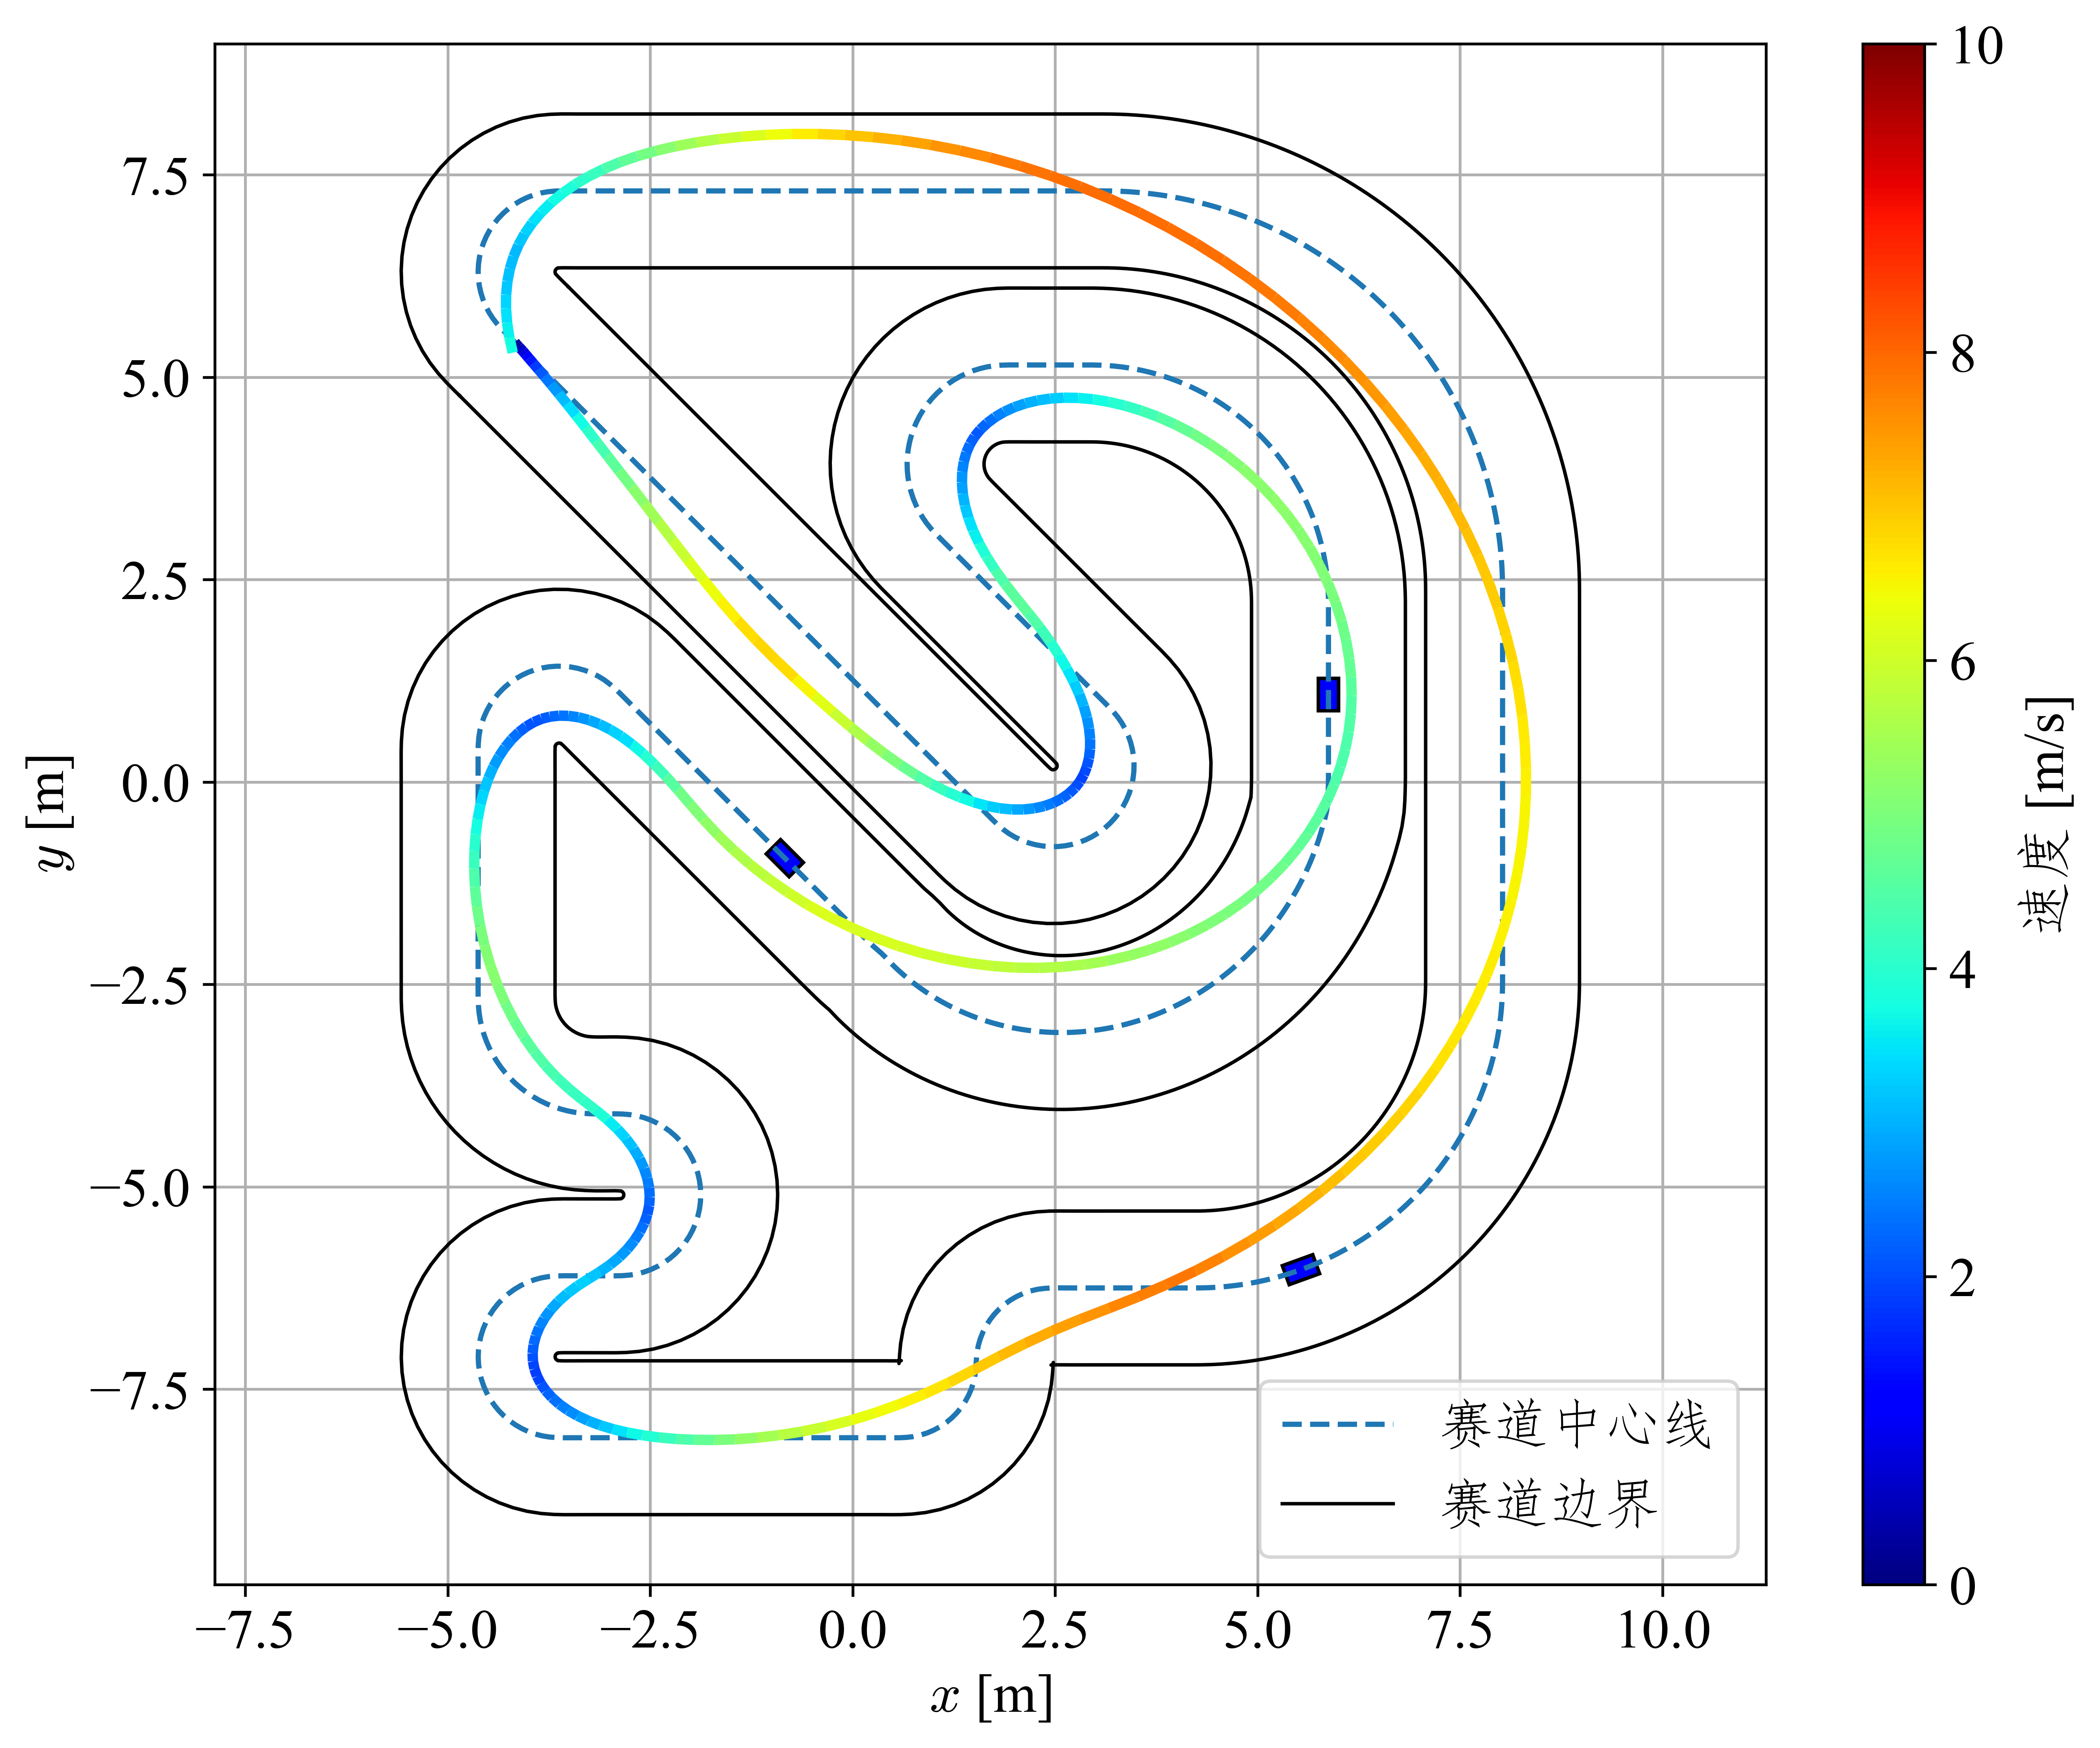
\includegraphics[width=0.33\linewidth]{figure/chapter2/mpcc_cbf_gamma0.7_static_trajectory.png}}
\subfloat[$\gamma=1.0$]{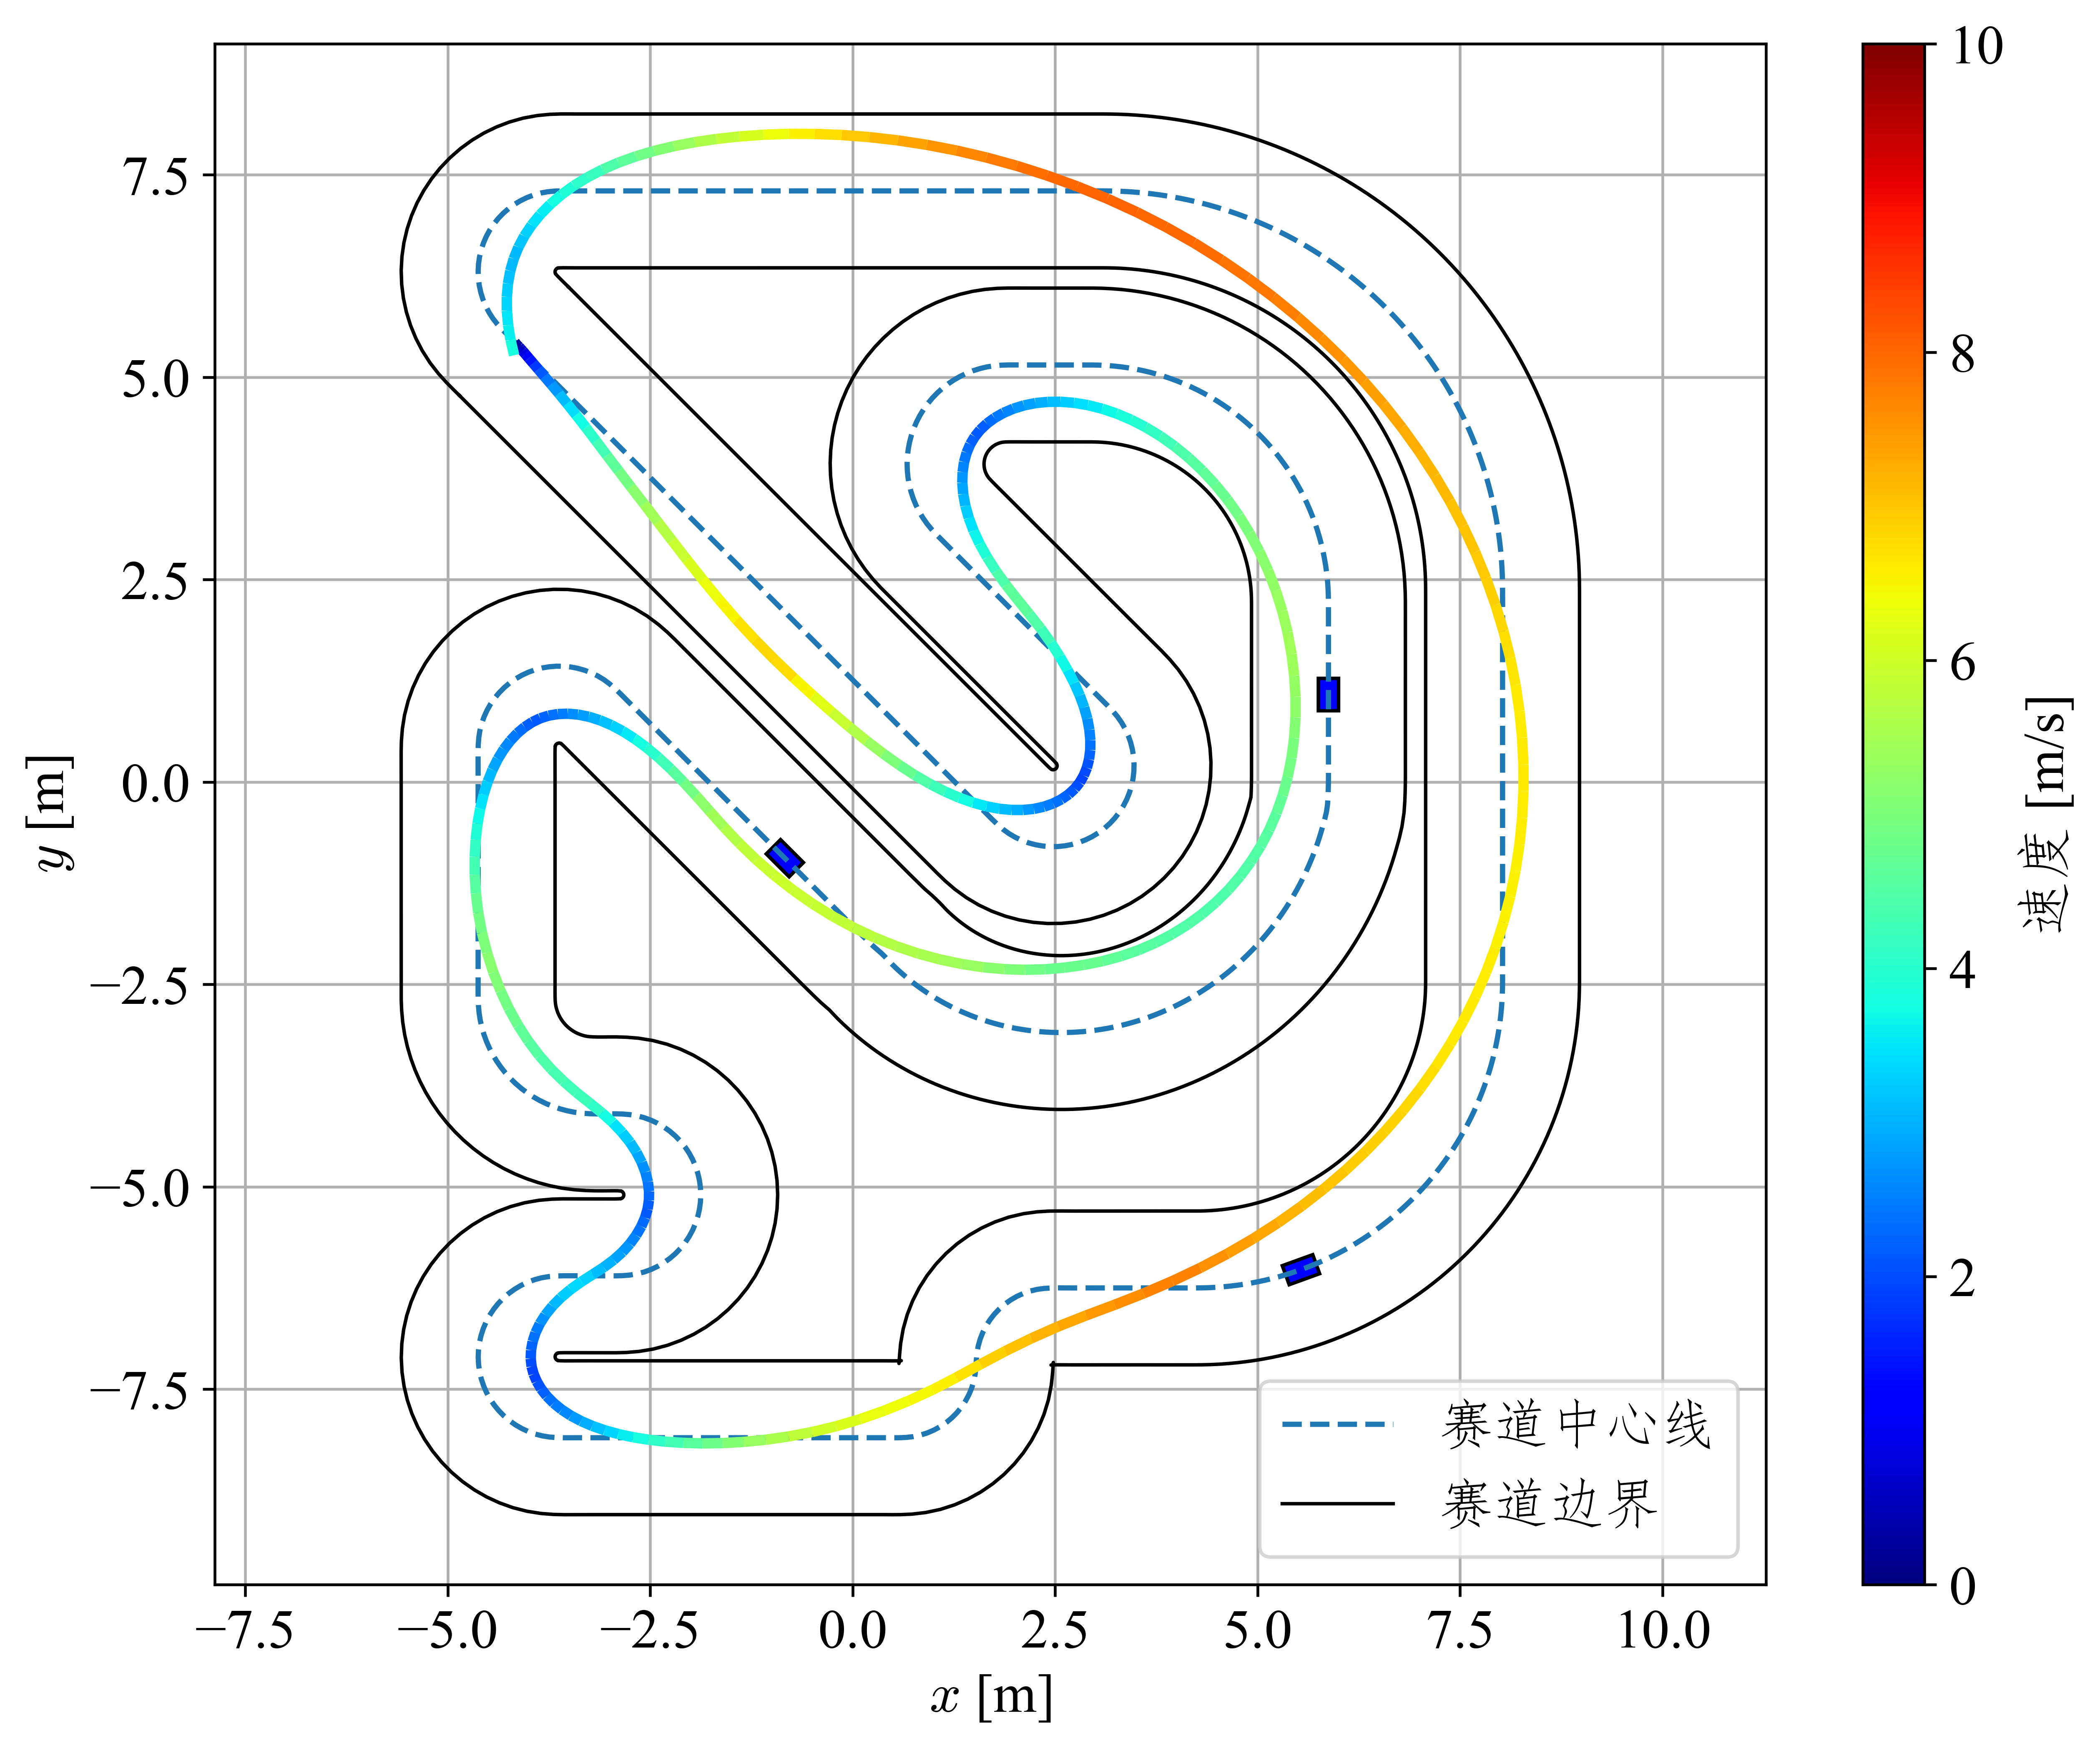
\includegraphics[width=0.33\linewidth]{figure/chapter2/mpcc_cbf_gamma1.0_static_trajectory.png}}
\caption{不同$\gamma$值下MPCC-CBF控制器的运动轨迹}
\label{fig:different-cbf-trajectory}
\end{figure}

\newpage
\subsection{动态超车实验与对比实验}
\begin{figure}[ht]
\centering
\subfloat[超越第一辆车]{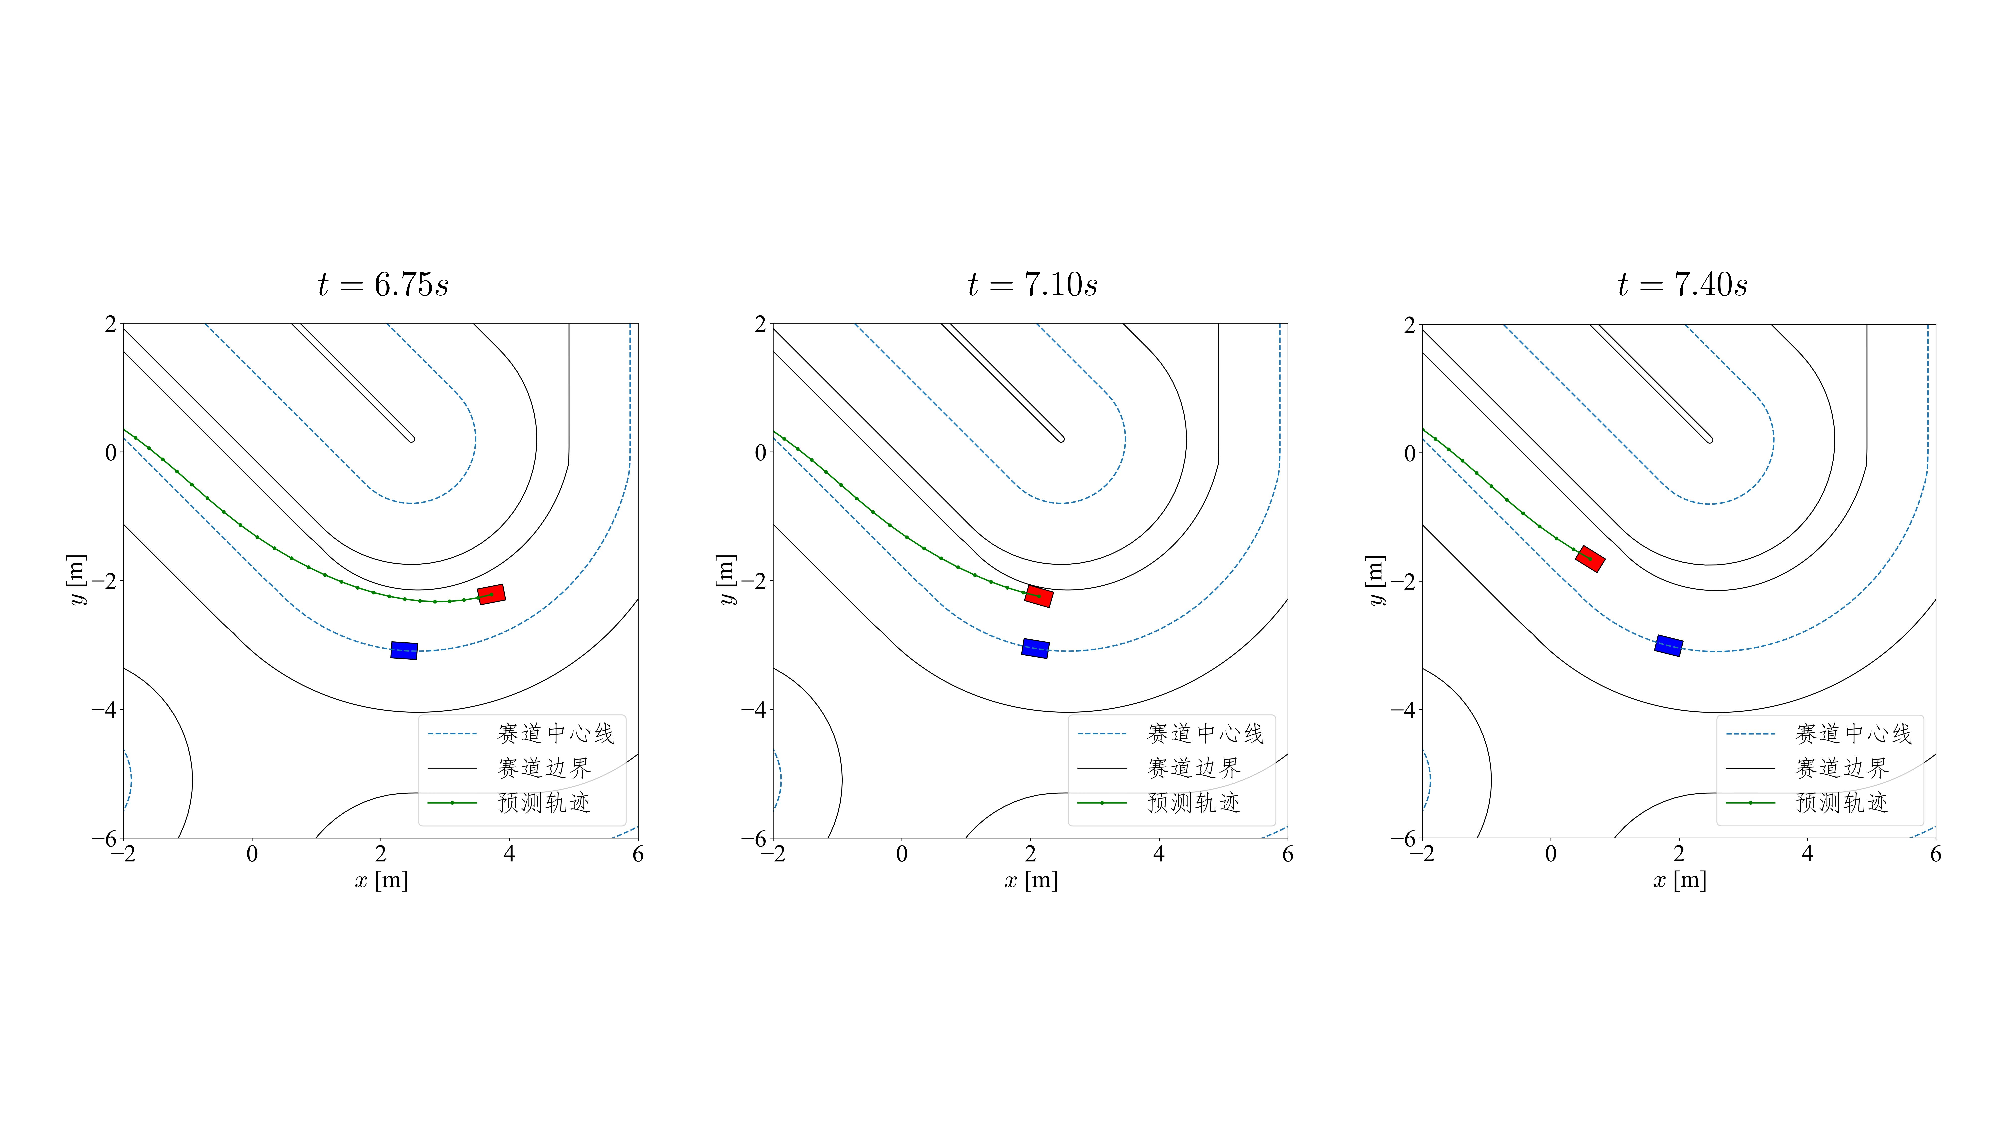
\includegraphics[width=0.9\linewidth]{figure/chapter2/overtake1.pdf}}

\subfloat[超越第二辆车]{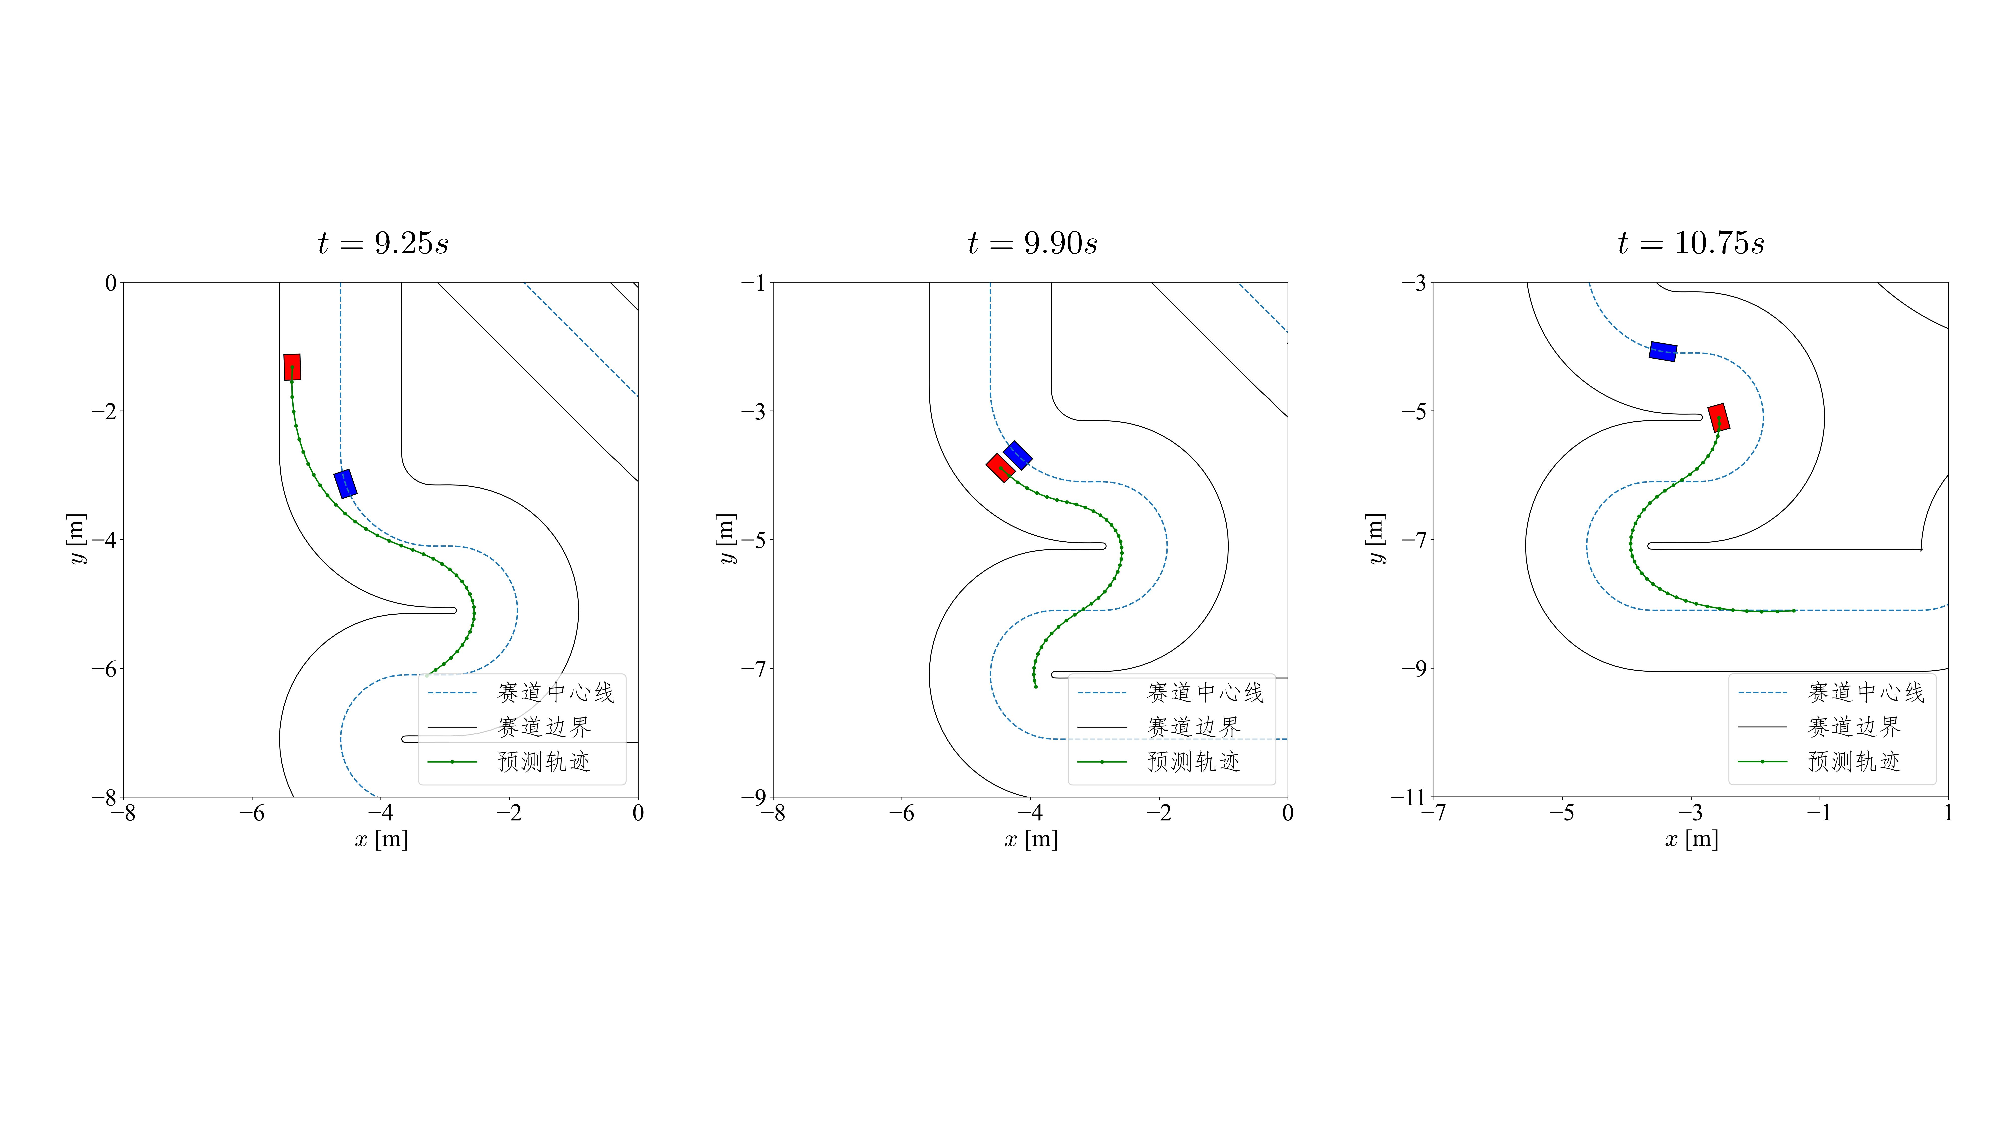
\includegraphics[width=0.9\linewidth]{figure/chapter2/overtake2.pdf}}

\subfloat[超越第三辆车]{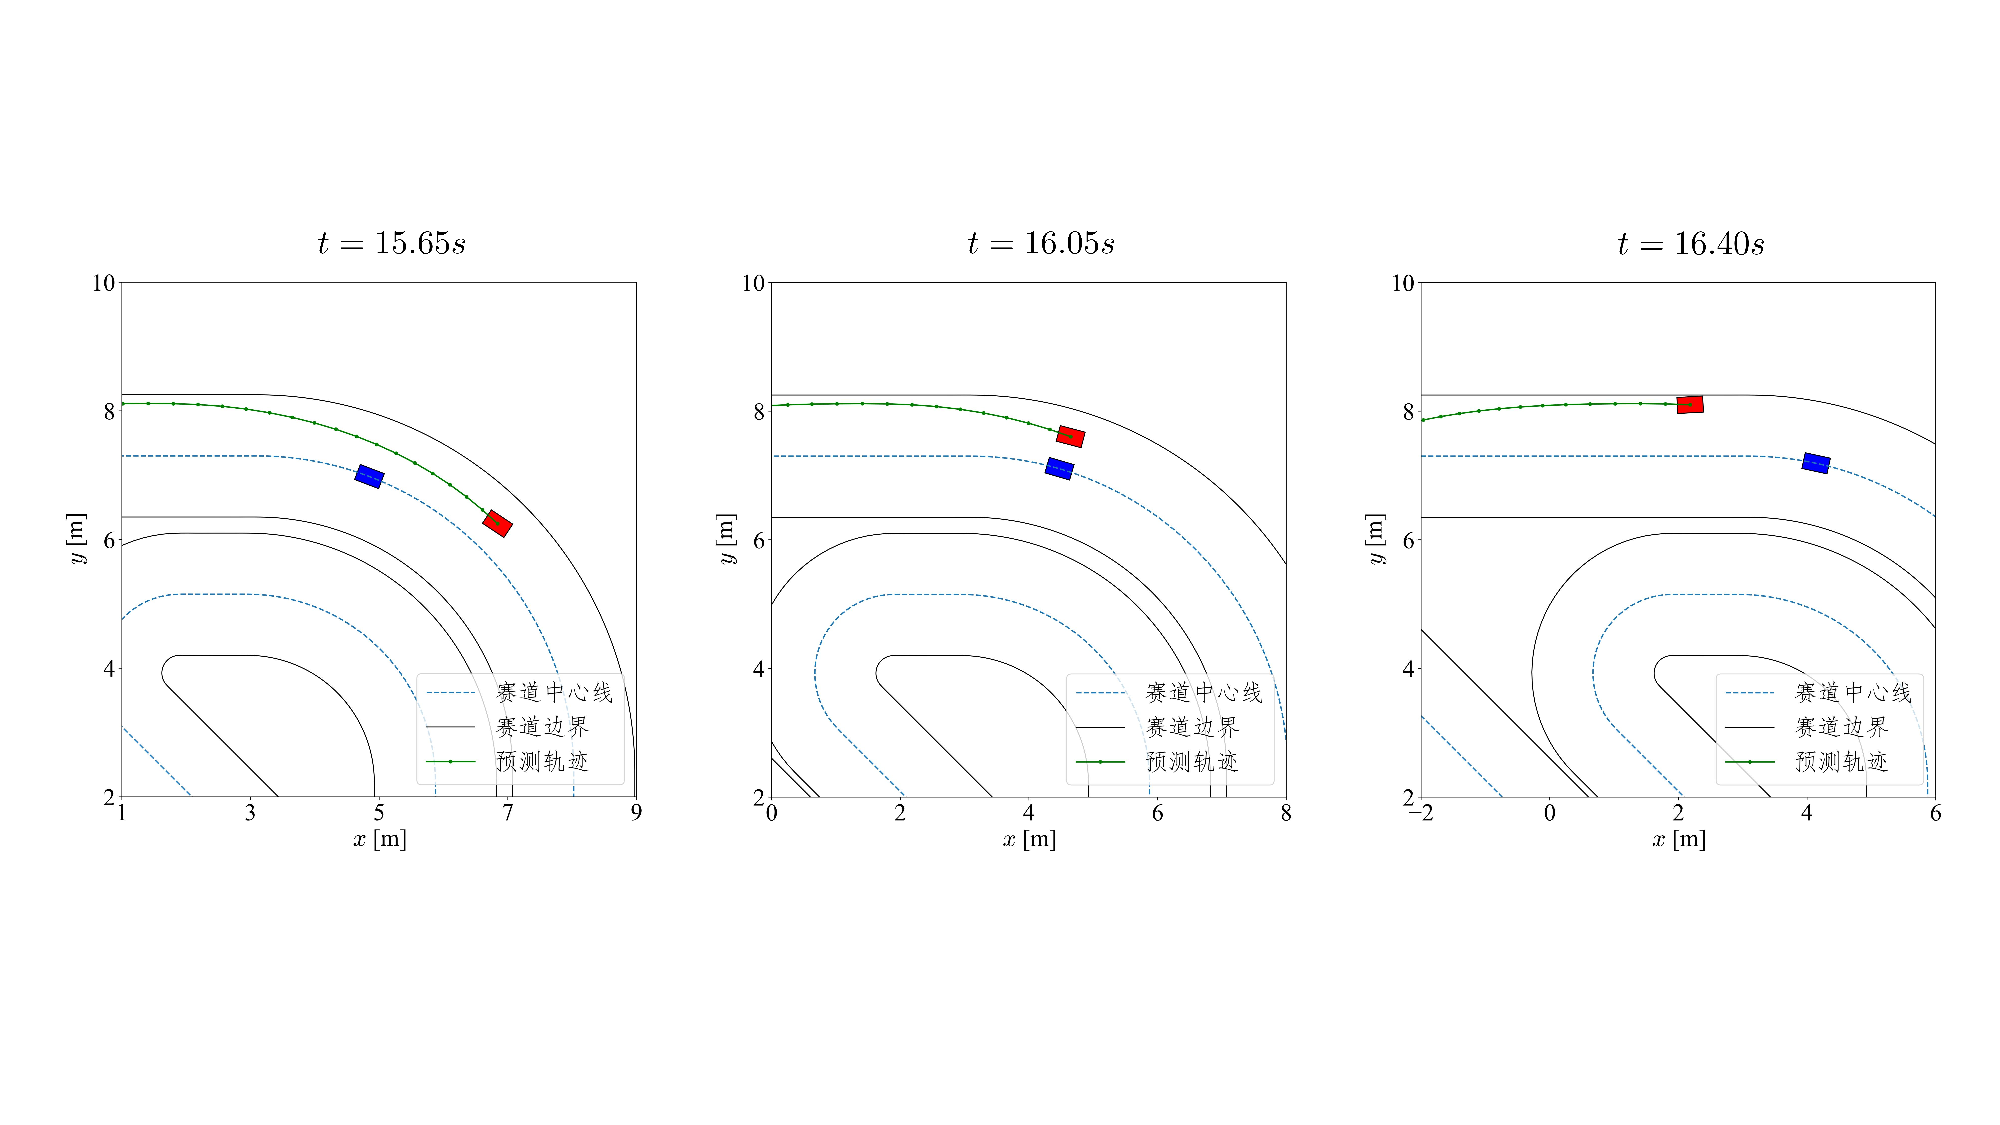
\includegraphics[width=0.9\linewidth]{figure/chapter2/overtake3.pdf}}
\caption{MPCC-CBF控制器在动态环境下的超车轨迹}
\label{fig:overtake-trajectory}
\end{figure}
接下来，我们在一个动态环境中验证了MPCC-CBF控制器的性能。仿真环境中有三辆其他赛车，分别以$1m/s$的速度行驶在赛道中心线上。我们将我们的赛车初始化在赛道中心线附近，并让其沿着赛道进行竞速控制，同时需要超越前方的三辆车。图\ref{fig:overtake-trajectory}展示了MPCC-CBF控制器在动态环境下的超车轨迹，其中红色车辆代表控制器控制的自身车辆，蓝色车辆代表其他车辆，绿色曲线代表MPCC-CBF控制器输出的最优轨迹。可以看出，赛车能够成功地超越前方的三辆车，同时保持安全距离，避免与赛道边界发生碰撞。

图\ref{fig:cbf-function}展示了在动态环境下控制障碍函数的变化曲线，图\ref{fig:mpcc-cbf-dynamic-control}展示了控制输入变化曲线。可以看出，在整个竞速过程中，赛道边界的控制障碍函数（图\ref{subfig:cbf-boundary}）和与其他车辆的控制障碍函数（图\ref{subfig:cbf-car}）都发生了明显的变化。当赛车接近赛道边界或其他车辆时，赛道边界的控制障碍函数值会迅速下降，提示控制器需要采取措施避免碰撞。从图像中可以看出，在超车和竞速时，控制器始终保持控制障碍函数值在安全范围内，即$h(x) \geq 0$，避免了潜在的碰撞风险。
\begin{figure}[ht]
\centering
\subfloat[与赛道边界的控制障碍函数]{\label{subfig:cbf-boundary}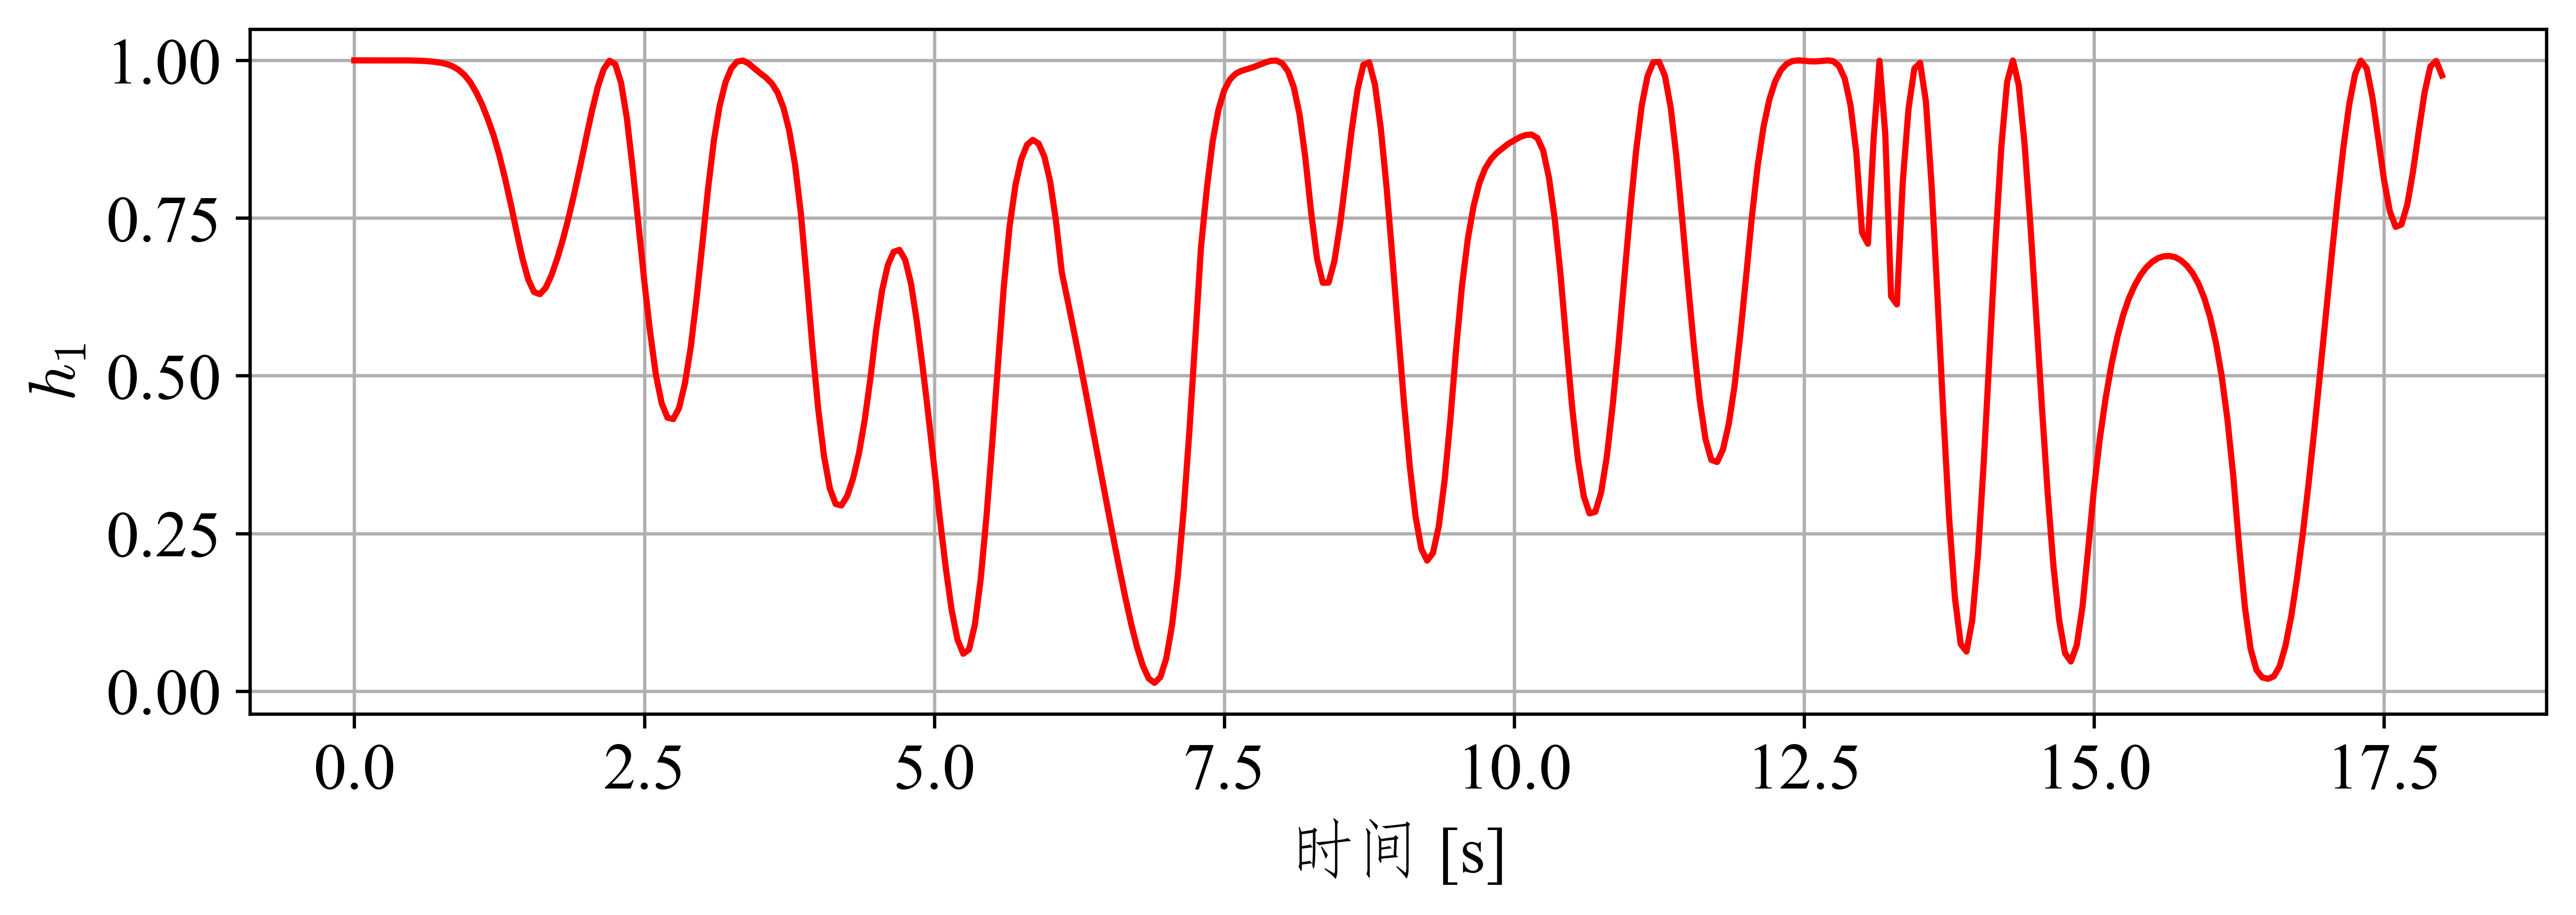
\includegraphics[width=0.5\linewidth]{figure/chapter2/mpcc_cbf_dynamic_cbf_boundary.png}}
\subfloat[与其他车辆的控制障碍函数]{\label{subfig:cbf-car}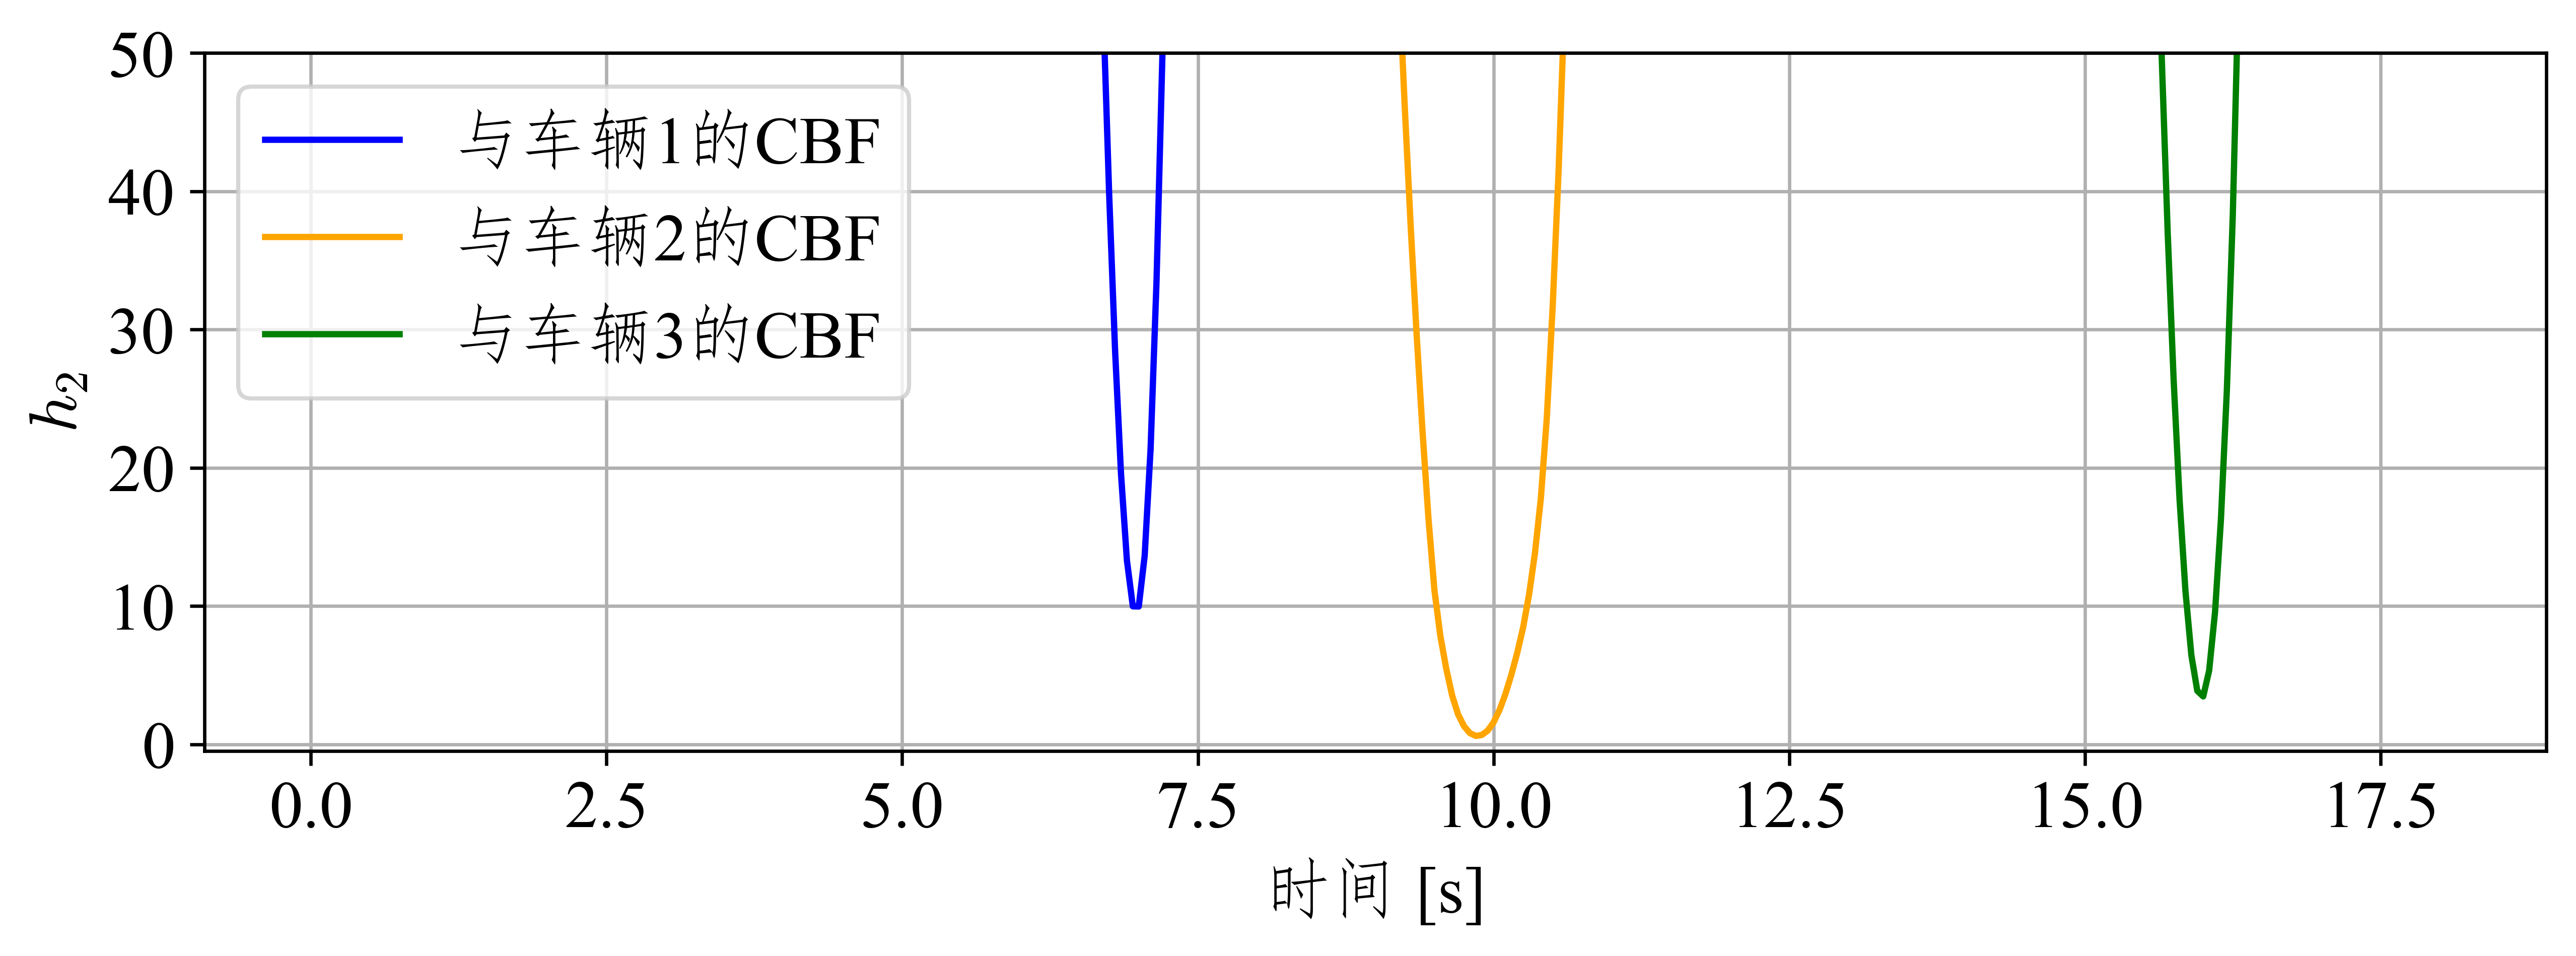
\includegraphics[width=0.5\linewidth]{figure/chapter2/mpcc_cbf_dynamic_cbf_car.png}}
\caption{动态环境下控制障碍函数的变化曲线}
\label{fig:cbf-function}
\end{figure}
\begin{figure}[ht]
    \centering
    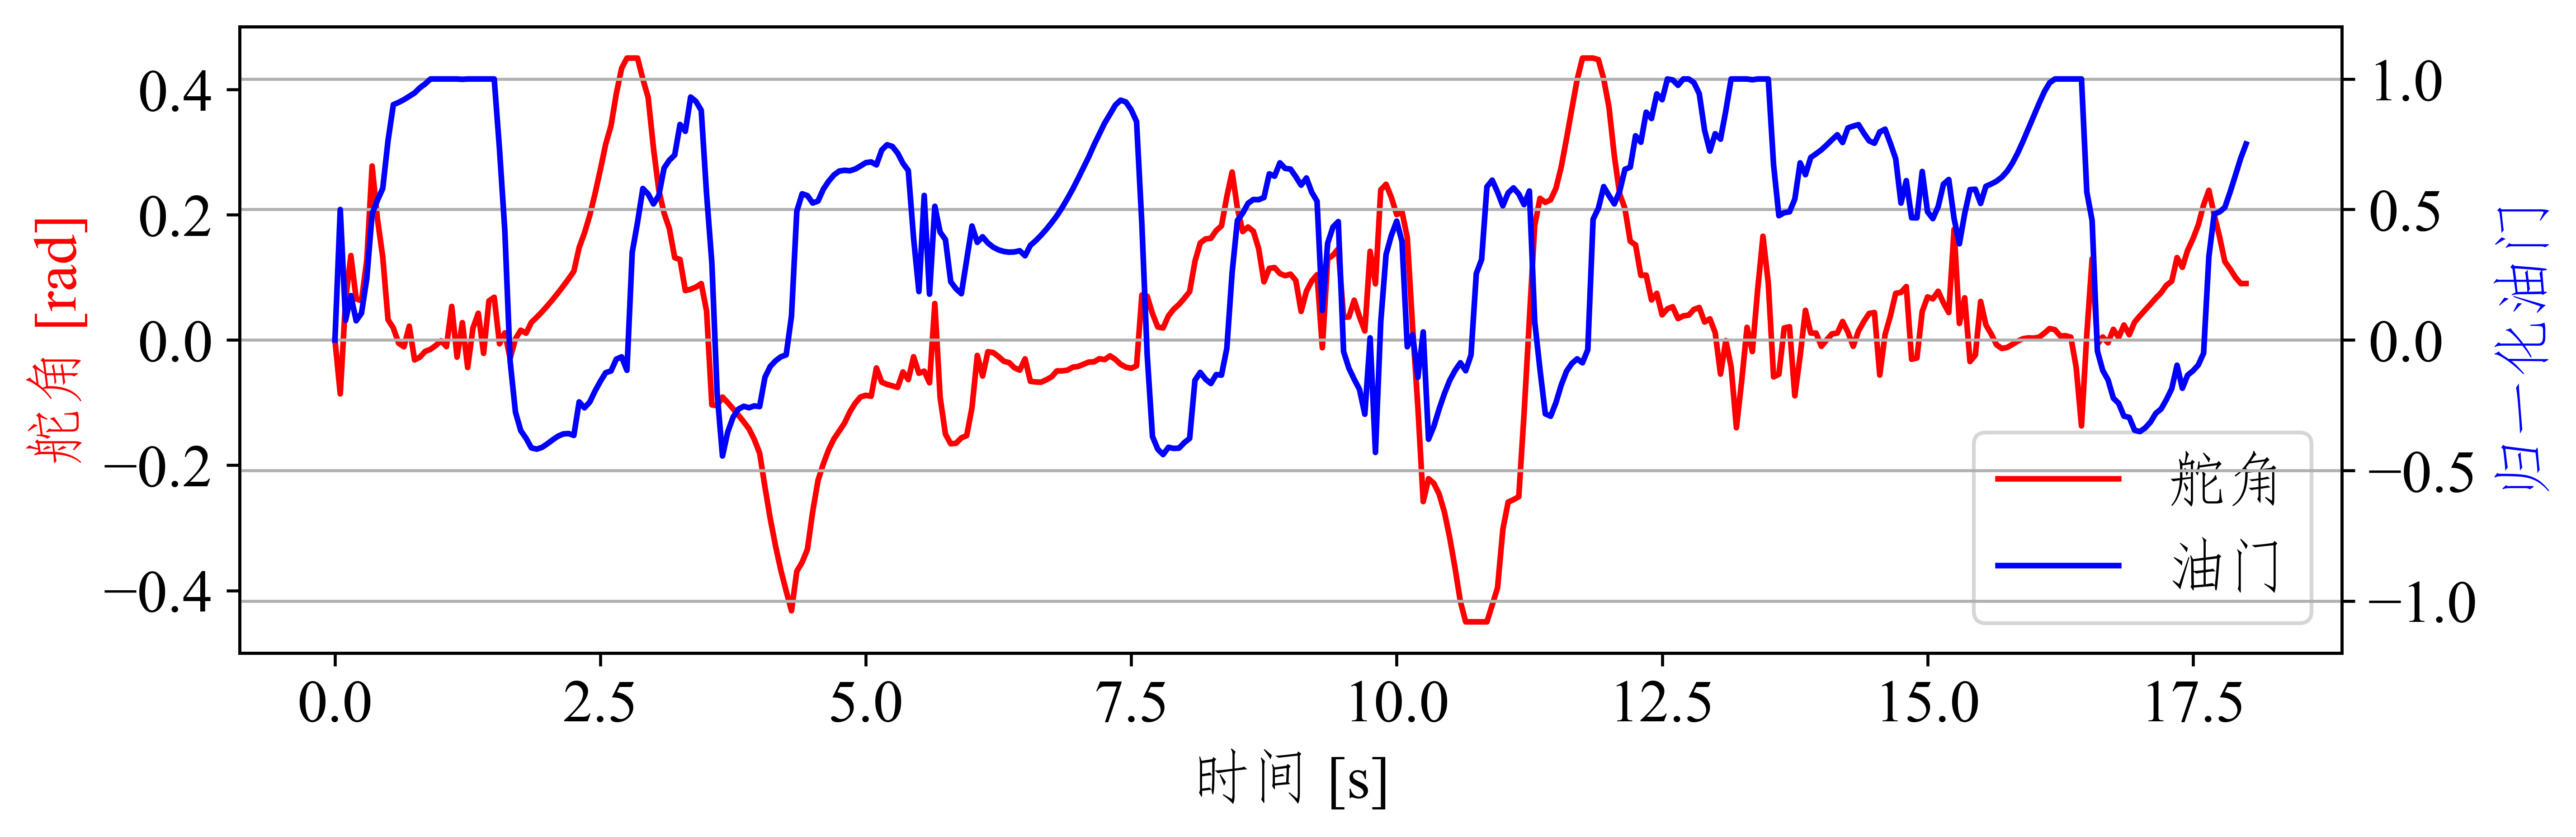
\includegraphics[width=0.7\linewidth]{figure/chapter2/mpcc_cbf_dynamic_control.png}
    \caption{MPCC-CBF控制器在动态环境下的控制输入变化曲线}
    \label{fig:mpcc-cbf-dynamic-control}
\end{figure}

为了进一步验证MPCC-CBF控制器在安全性和性能之间的权衡能力，我们将其与普通的MPCC控制器、以及一个传统轨迹优化算法\cite{heilmeier2020minimum}+Pure Pursuit轨迹跟踪控制器\cite{coulter1992implementation}（Trajectory Optimization + Pure Pursuit, 简称TO+PP）在静态环境中进行比较。轨迹优化算法最小化轨迹的累积曲率来生成一条平滑的参考轨迹，Pure Pursuit控制器则通过计算一个前视点来实现对参考轨迹的跟踪。表\ref{tab:controller-comparison}展示了三种控制器在单圈时间、距障碍物最小距离、平均速度和最大速度等指标上的比较结果。可以看出，MPCC控制器的单圈时间最短，平均速度和最大速度最高，但距障碍物的最小距离最小，安全性较低；MPCC-CBF控制器在单圈时间、平均速度和最大速度方面略逊于普通的MPCC控制器，但在距障碍物的最小距离方面明显优于普通的MPCC控制器，安全性更高；TO+PP控制器的单圈时间最长，与障碍物距离也较小。
\begin{table}[h]
    \caption{\label{tab:controller-comparison}不同控制器性能比较}
    \renewcommand\arraystretch{1.25}
    \setlength{\tabcolsep}{6pt}{
    \begin{tabular}{ccccc}
    \toprule[2pt]
        控制器 & 单圈时间[s] & 距障碍物最小距离[m] & 平均速度[m/s] & 最大速度[m/s] \\ \midrule[1pt]
        TO+PP     & $22.50$  & $0.297$ & $3.50$ & $7.27$ \\
        MPCC     & $17.40$  & $0.248$ & $4.47$ & $8.01$ \\
        MPCC-CBF     & $17.45$  & $0.447$ & $4.46$ & $7.98$ \\ \bottomrule[2pt]
    \end{tabular}}
\end{table}

为了模仿真实环境中的不确定性，我们在仿真环境中引入了状态估计误差和模型参数误差，用于评估不同控制器在不确定环境下的安全性。状态估计误差通过在车辆的位置变量上添加一个均值为0，标准差为$\sigma_1$的高斯噪声来模拟。模型参数误差通过在车辆动力学模型中的摩擦系数上添加一个均值为0，标准差为$\sigma_2$的高斯噪声来模拟。所有控制器分别在不同$\sigma_1$和$\sigma_2$值下进行了仿真测试，每次测试进行了40次运行，完成一圈竞速视为成功，图\ref{fig:uncertainty-comparison}展示了不同控制器在不同不确定性水平下的成功率比较结果。可以看出，随着不确定性水平的增加，所有控制器的成功率都在下降，但MPCC-CBF控制器的成功率下降幅度最小，表现出更强的鲁棒性和安全性。
\begin{figure}[ht]
\centering
\subfloat[状态估计不确定环境]{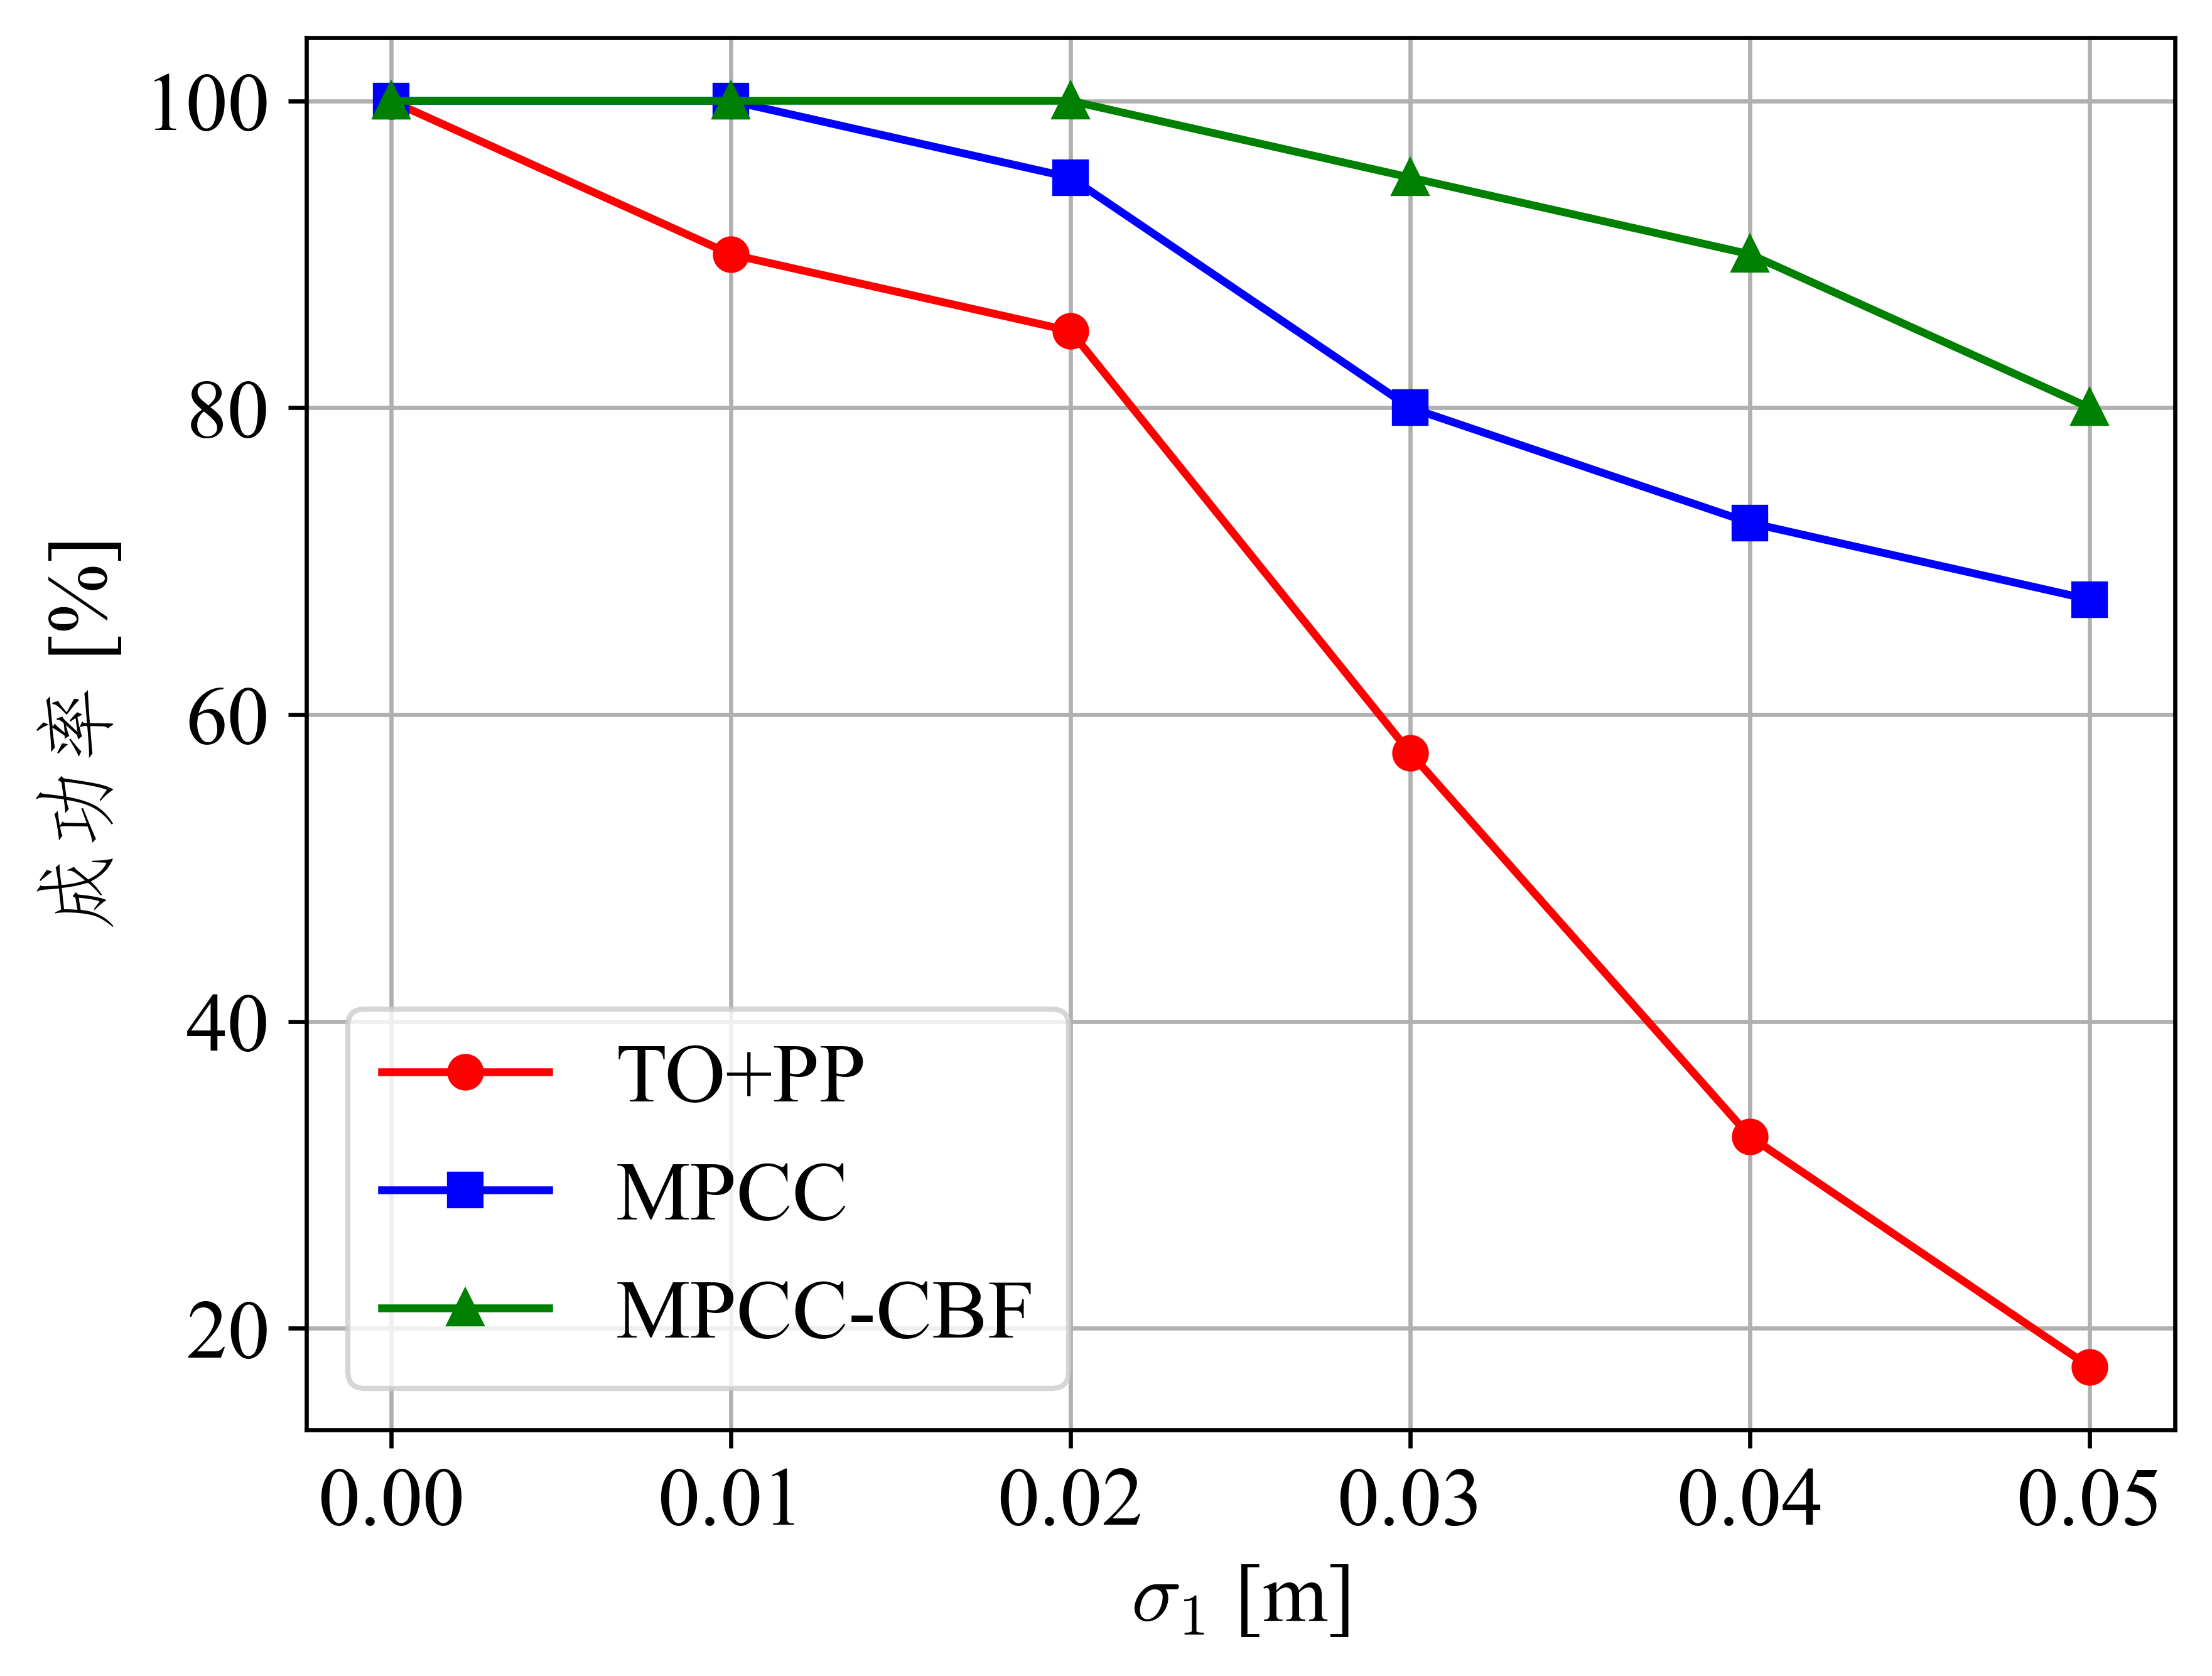
\includegraphics[width=0.45\linewidth]{figure/chapter2/uncertainty_comparison_state_estimation.png}}
\subfloat[模型参数不确定环境]{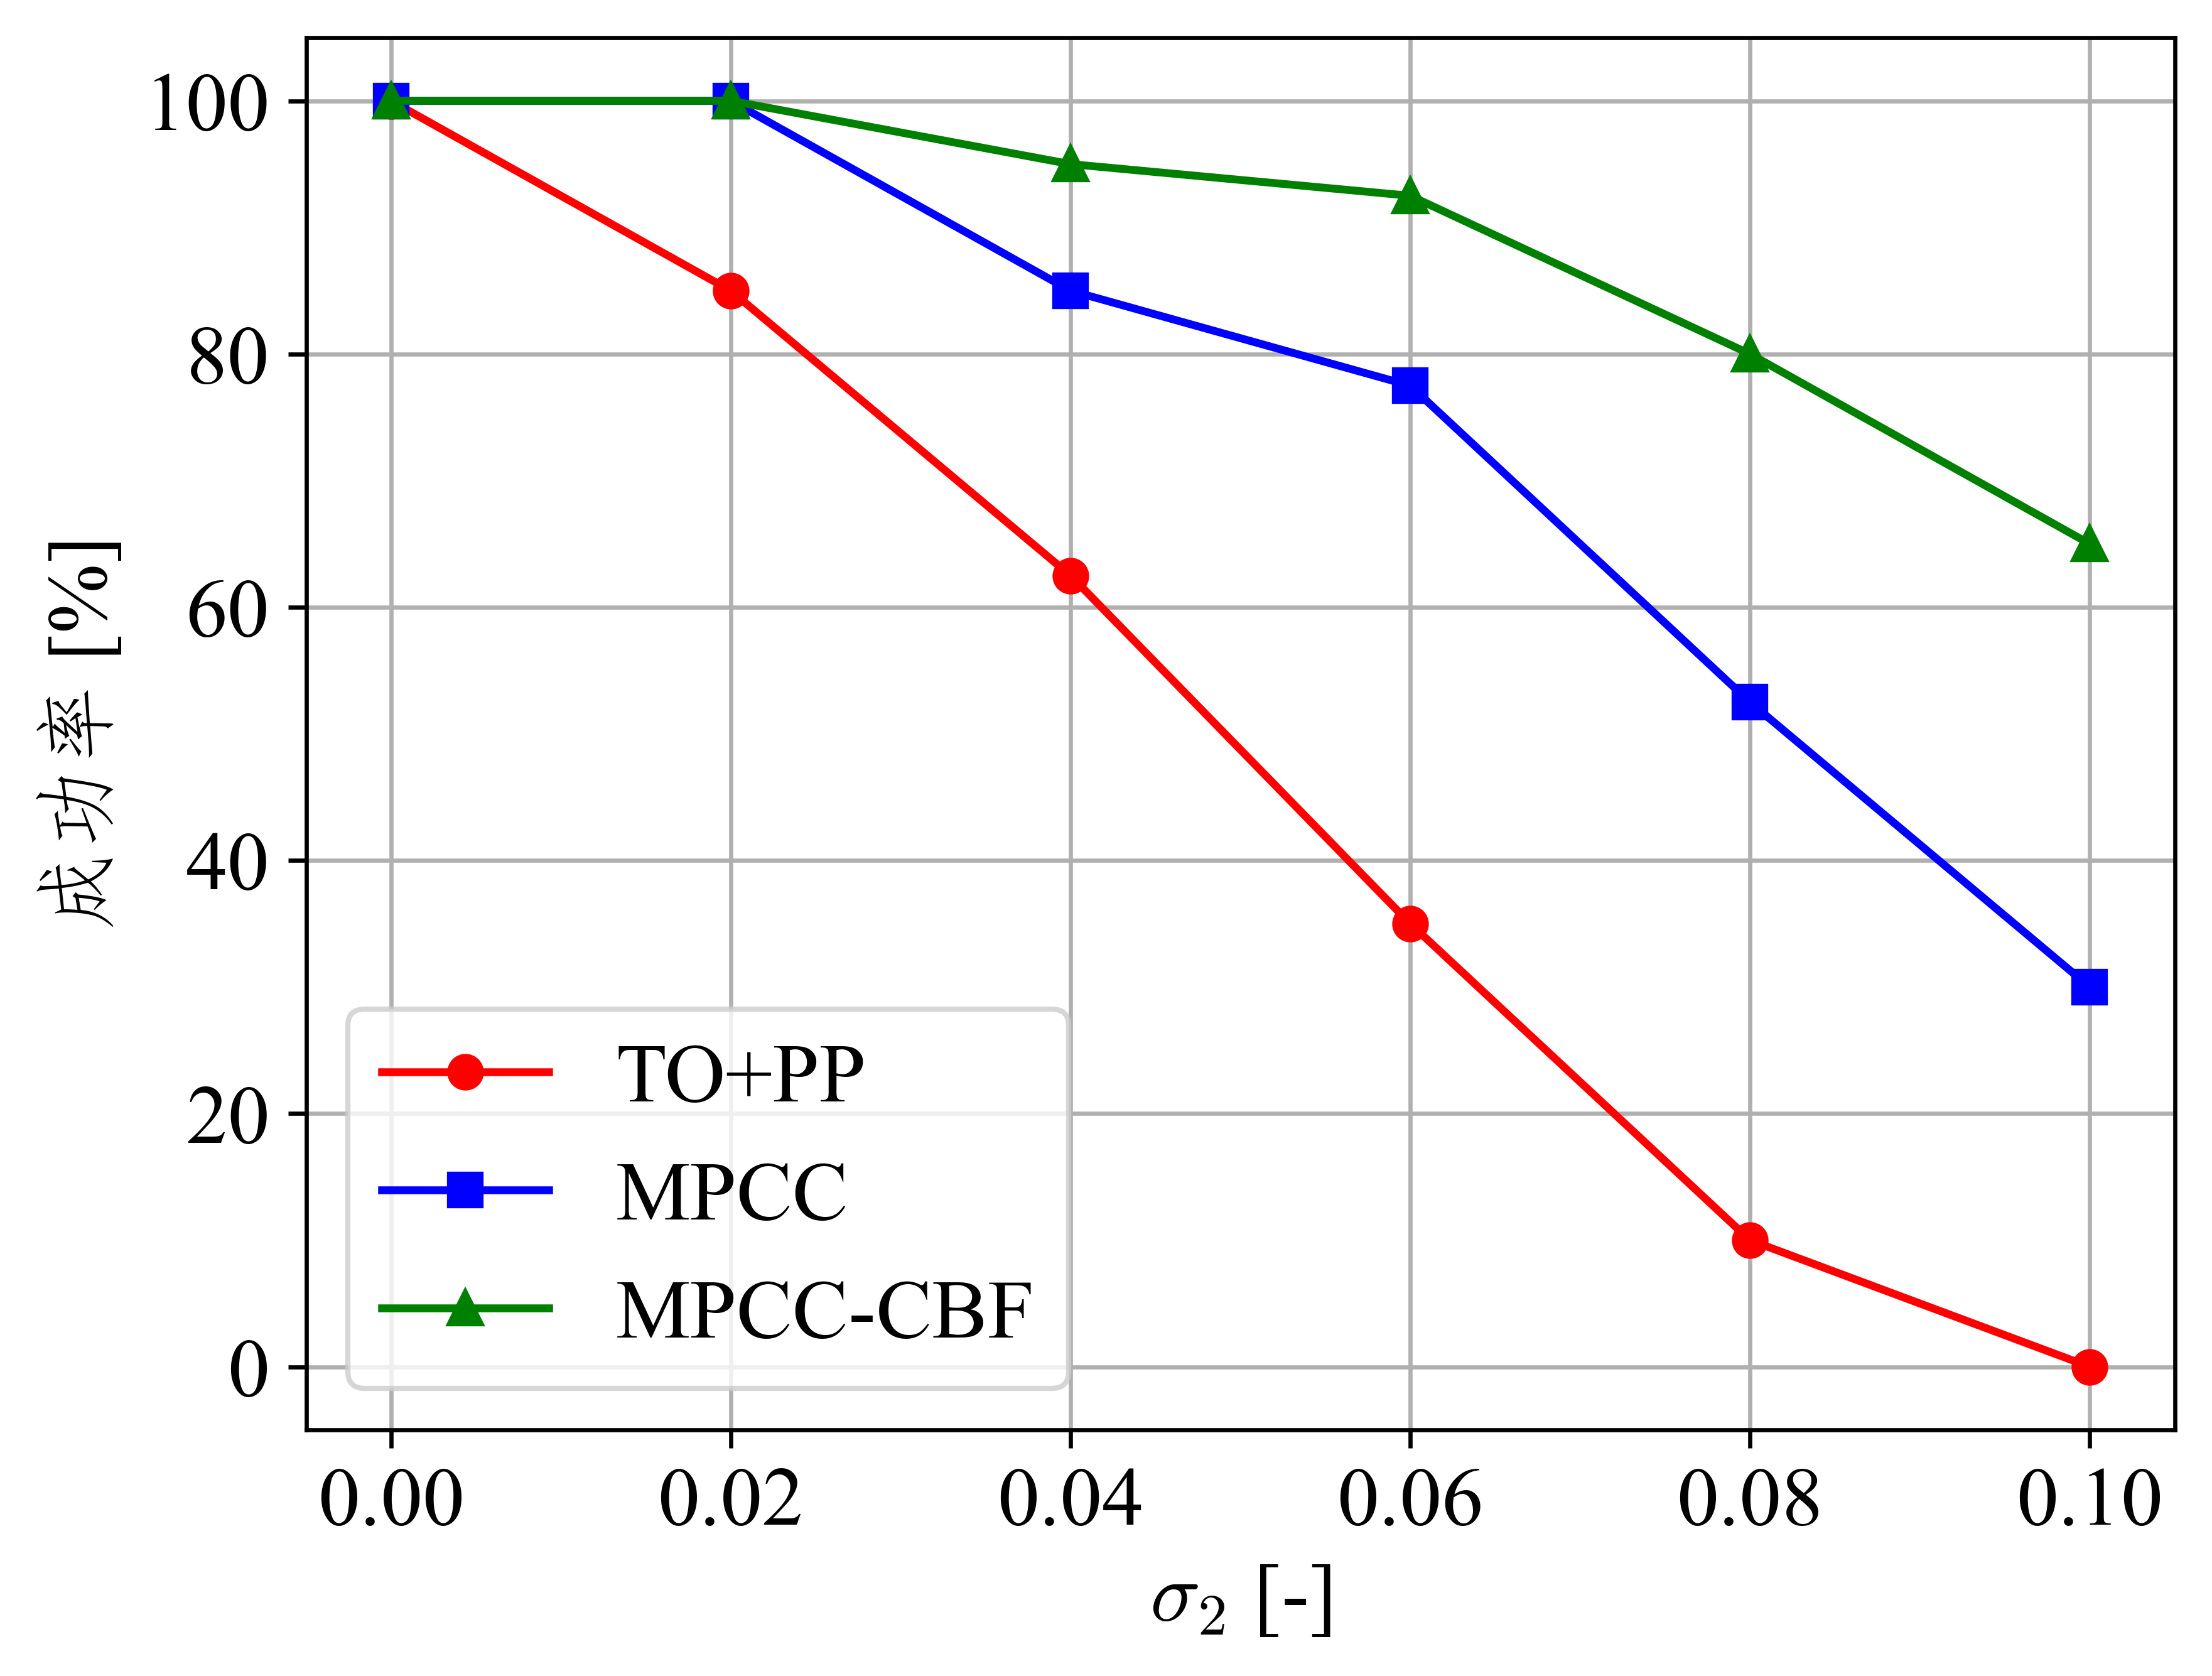
\includegraphics[width=0.45\linewidth]{figure/chapter2/uncertainty_comparison_model_parameter.png}}
\caption{不同控制器在不确定环境中的成功率比较}
\label{fig:uncertainty-comparison}
\end{figure}

\newpage
\subsection{实车实验与结果分析}
本文使用了一个基于ROS的实车系统架构来实现MPCC-CBF控制器，并在真实环境中进行了验证。赛车硬件平台如图\ref{subfig:car-platform}所示，系统架构如图\ref{subfig:real-system}所示，主要包括以下几个模块：（1）状态估计模块：利用拓展卡尔曼滤波算法，融合IMU数据和动作捕捉系统提供的位置信息来估计车辆的状态信息；（2）环境感知模块：通过激光雷达传感器来感知周围环境，建立地图识别赛道边界，根据自身位置来提取赛道中心线，从而得知赛道信息先验；（3）MPCC-CBF控制模块：MPCC-CBF控制器，根据当前状态和环境信息来计算最优的控制输入，实车实验中控制器在一台Intel NUC 12Pro机载计算机上运行；（4）底层执行模块：使用VESC电子调速器将MPCC-CBF控制模块输出的控制输入转换为底盘执行器的命令，并发送给车辆的执行系统。
\begin{figure}[ht]
\centering
\subfloat[自动驾驶赛车硬件平台]{\label{subfig:car-platform}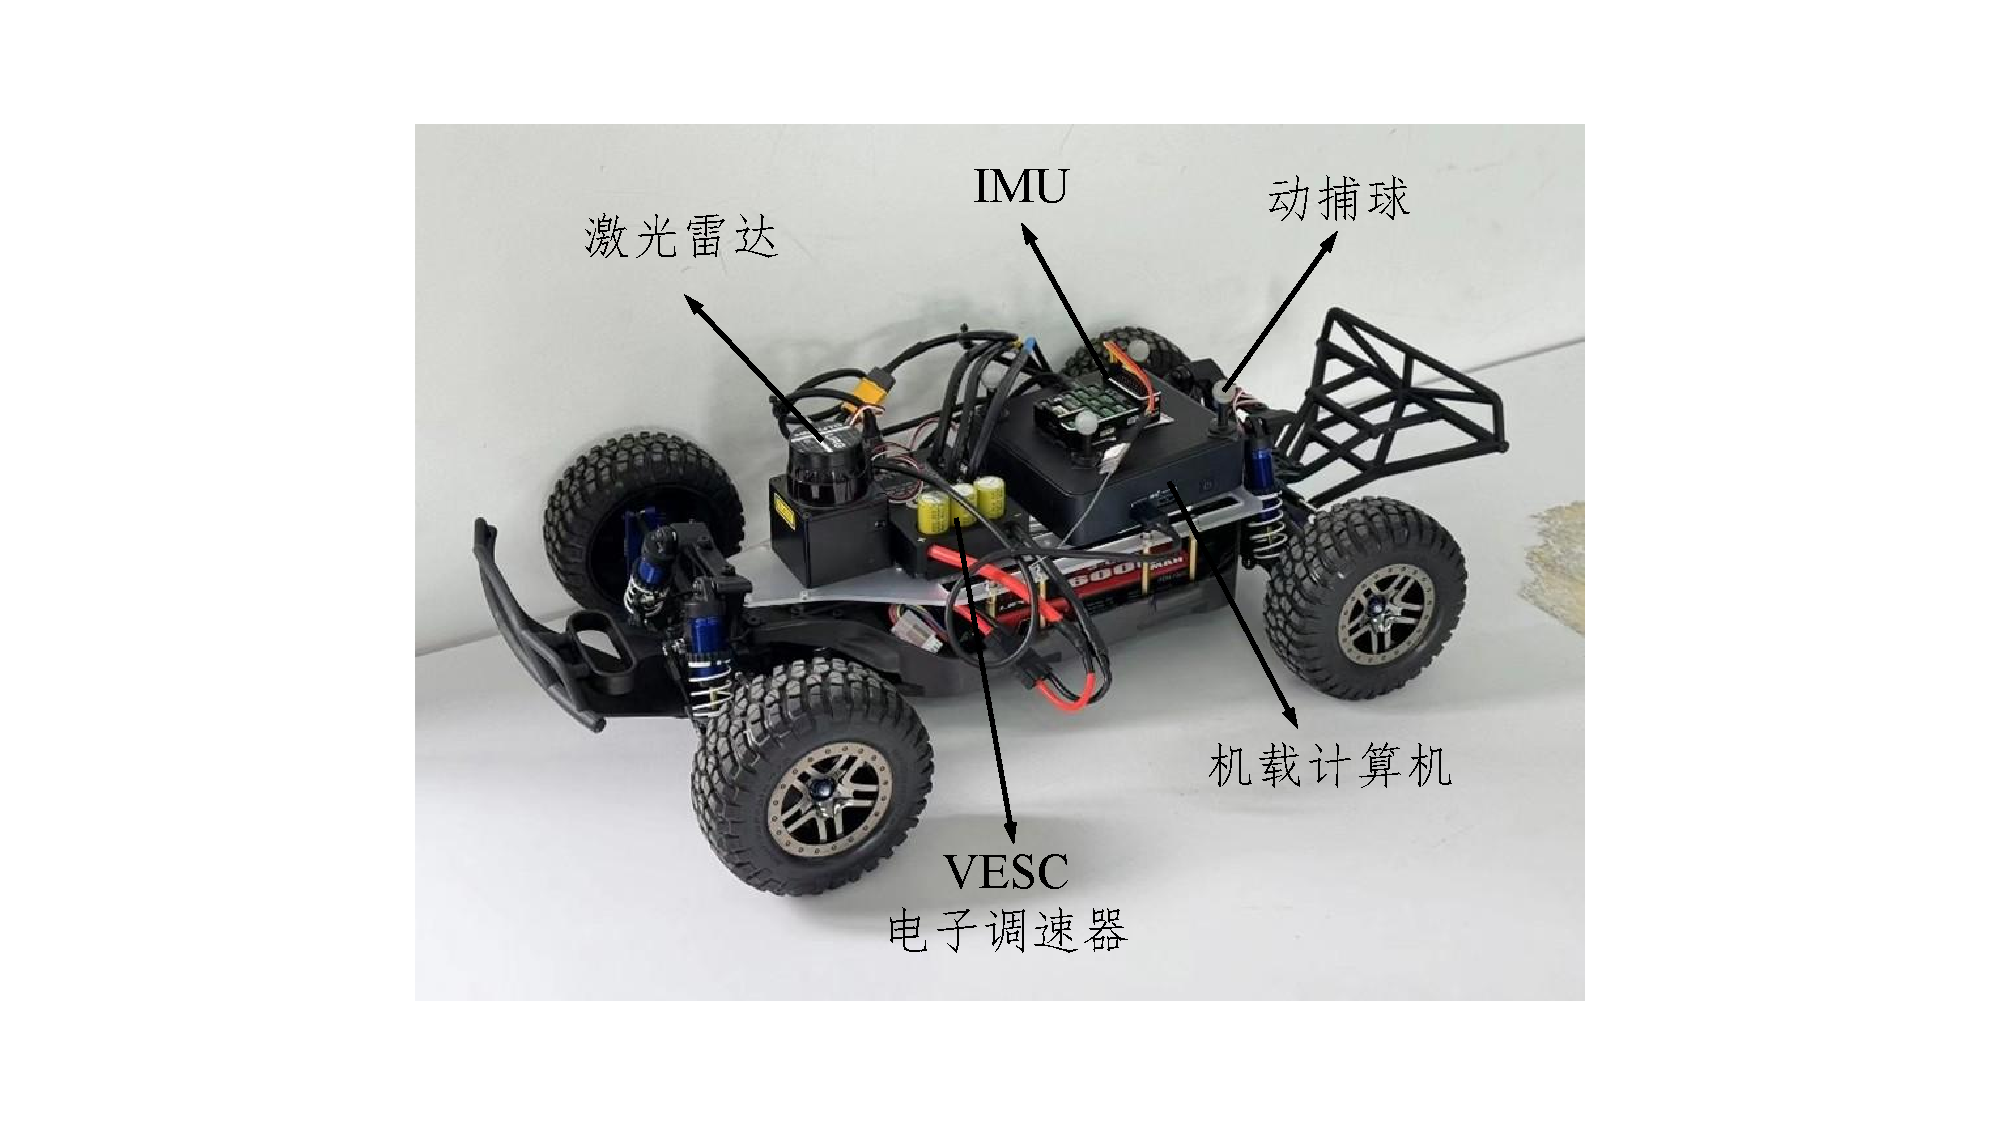
\includegraphics[width=0.4\linewidth]{figure/chapter2/car-system.pdf}}
\subfloat[实车系统架构]{\label{subfig:real-system}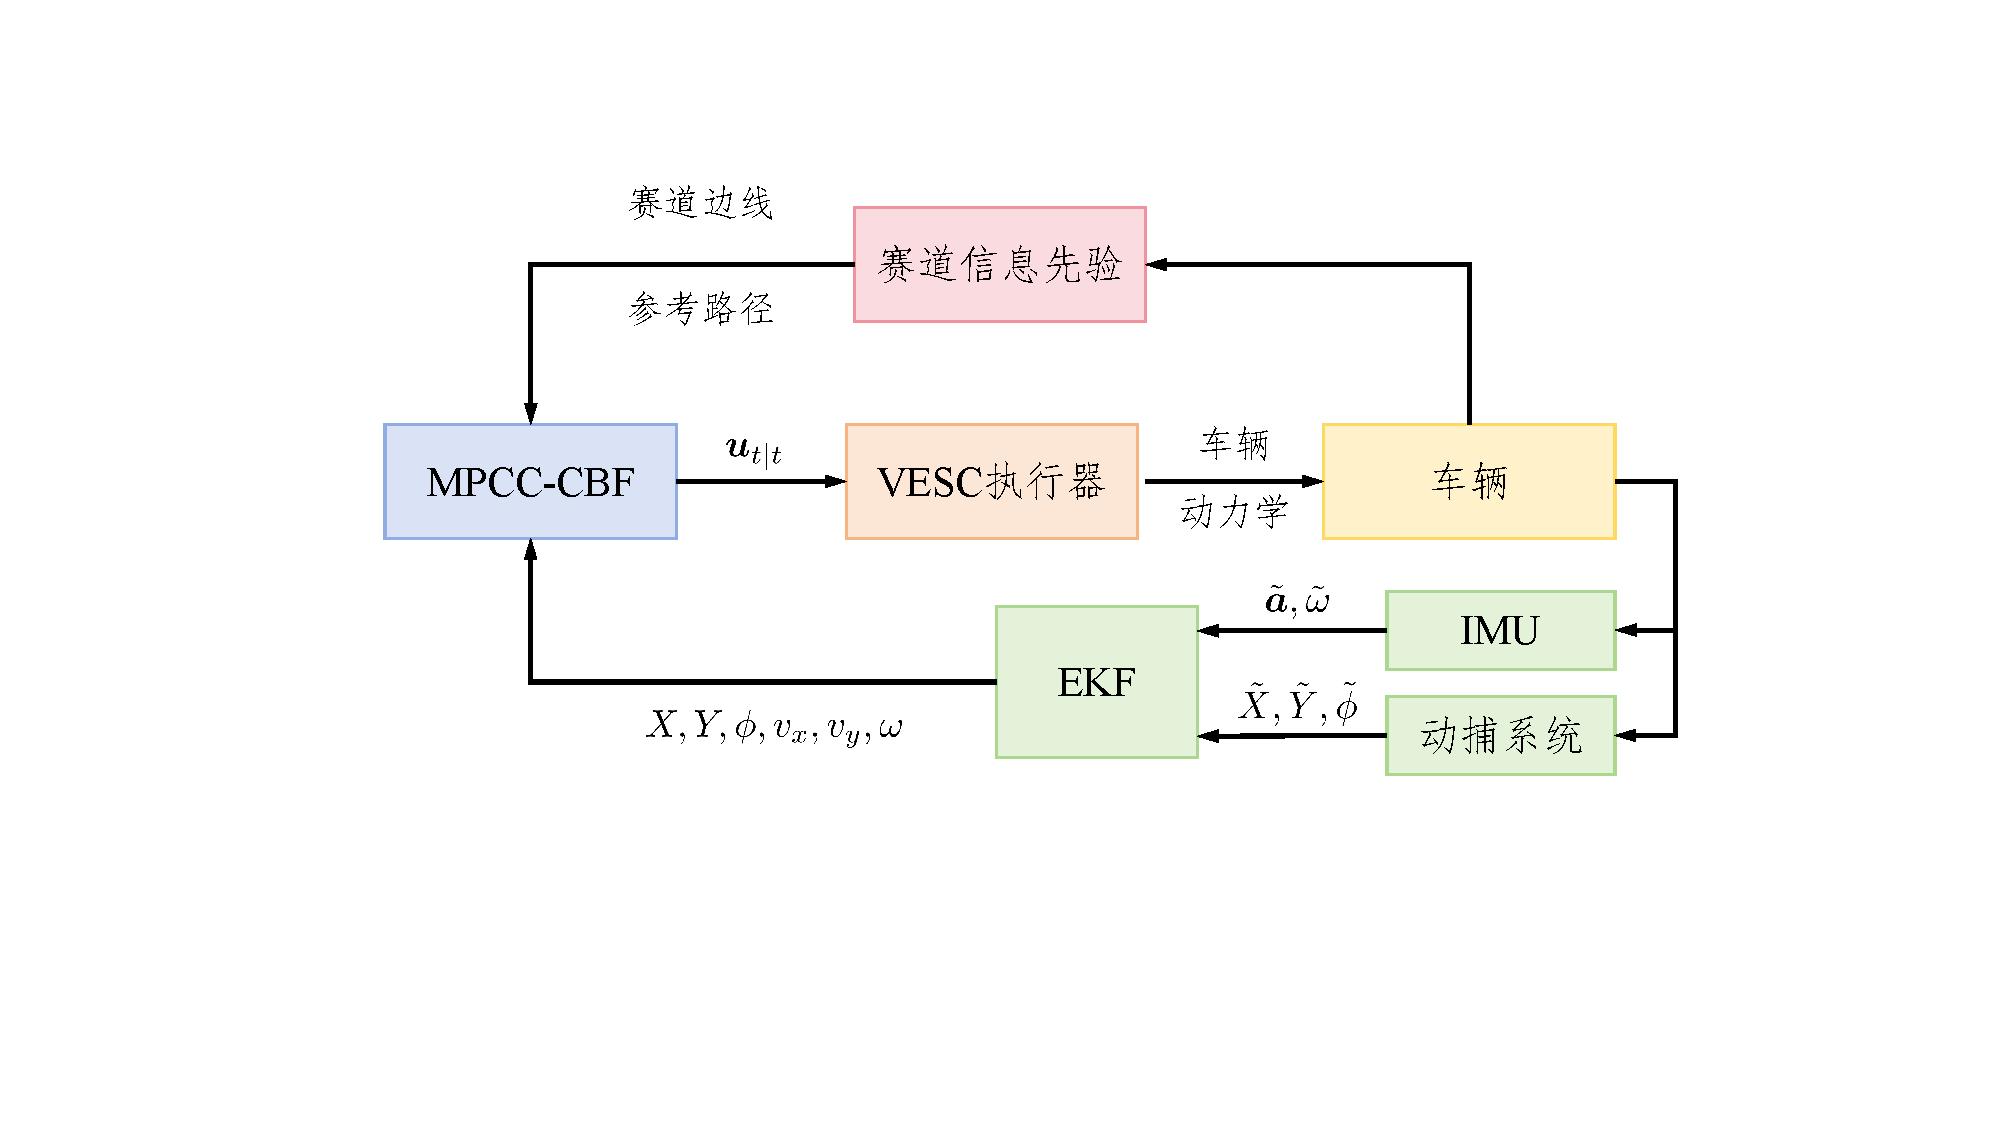
\includegraphics[width=0.6\linewidth]{figure/chapter2/mpcc-cbf-real-system.pdf}}
\caption{赛车硬件平台与系统架构}
\label{fig:car-platform-and-system}
\end{figure}

实车实验在一个长为13m，宽为7m的赛道上进行，如图\ref{fig:real-map}所示。本文中采用了Cartographer算法\cite{hess2016real}作为地图构建算法，构建好地图后手动遥控赛车在赛道上行驶一圈来记录赛车定位，并经过一次平滑处理后得到赛道中心线。赛道中心线被离散化为100个点，并通过三次样条插值来生成连续的赛道中心线函数。实车实验中，MPCC-CBF控制器以50Hz的频率进行控制输入的计算和更新，以实现实时的竞速控制。

实车实验中，MPCC-CBF控制器能够成功地控制赛车沿着赛道进行竞速，同时保持安全距离，避免与赛道边界发生碰撞。图\ref{fig:real-trajectory}展示了实车实验中的运动轨迹，图\ref{fig:real-cbf}展示了控制障碍函数的变化曲线，图\ref{fig:real-control}展示了对应的控制输入变化曲线，表\ref{tab:real-experiment-results}展示了实车实验的结果。可以看出，实物赛车可以安全高速地完成竞速任务；控制输入的变化也比较平滑；滞后误差较小，控制器能准确估计赛车在赛道上的位置。在拐入弯道时，赛车采用入弯前外侧、入弯内侧、出弯外侧的行驶策略来提高过弯性能。CBF值在整个竞速过程中始终保持在安全范围内，即$h(x) \geq 0$，避免了潜在的碰撞风险。
\begin{figure}[H]
    \centering
    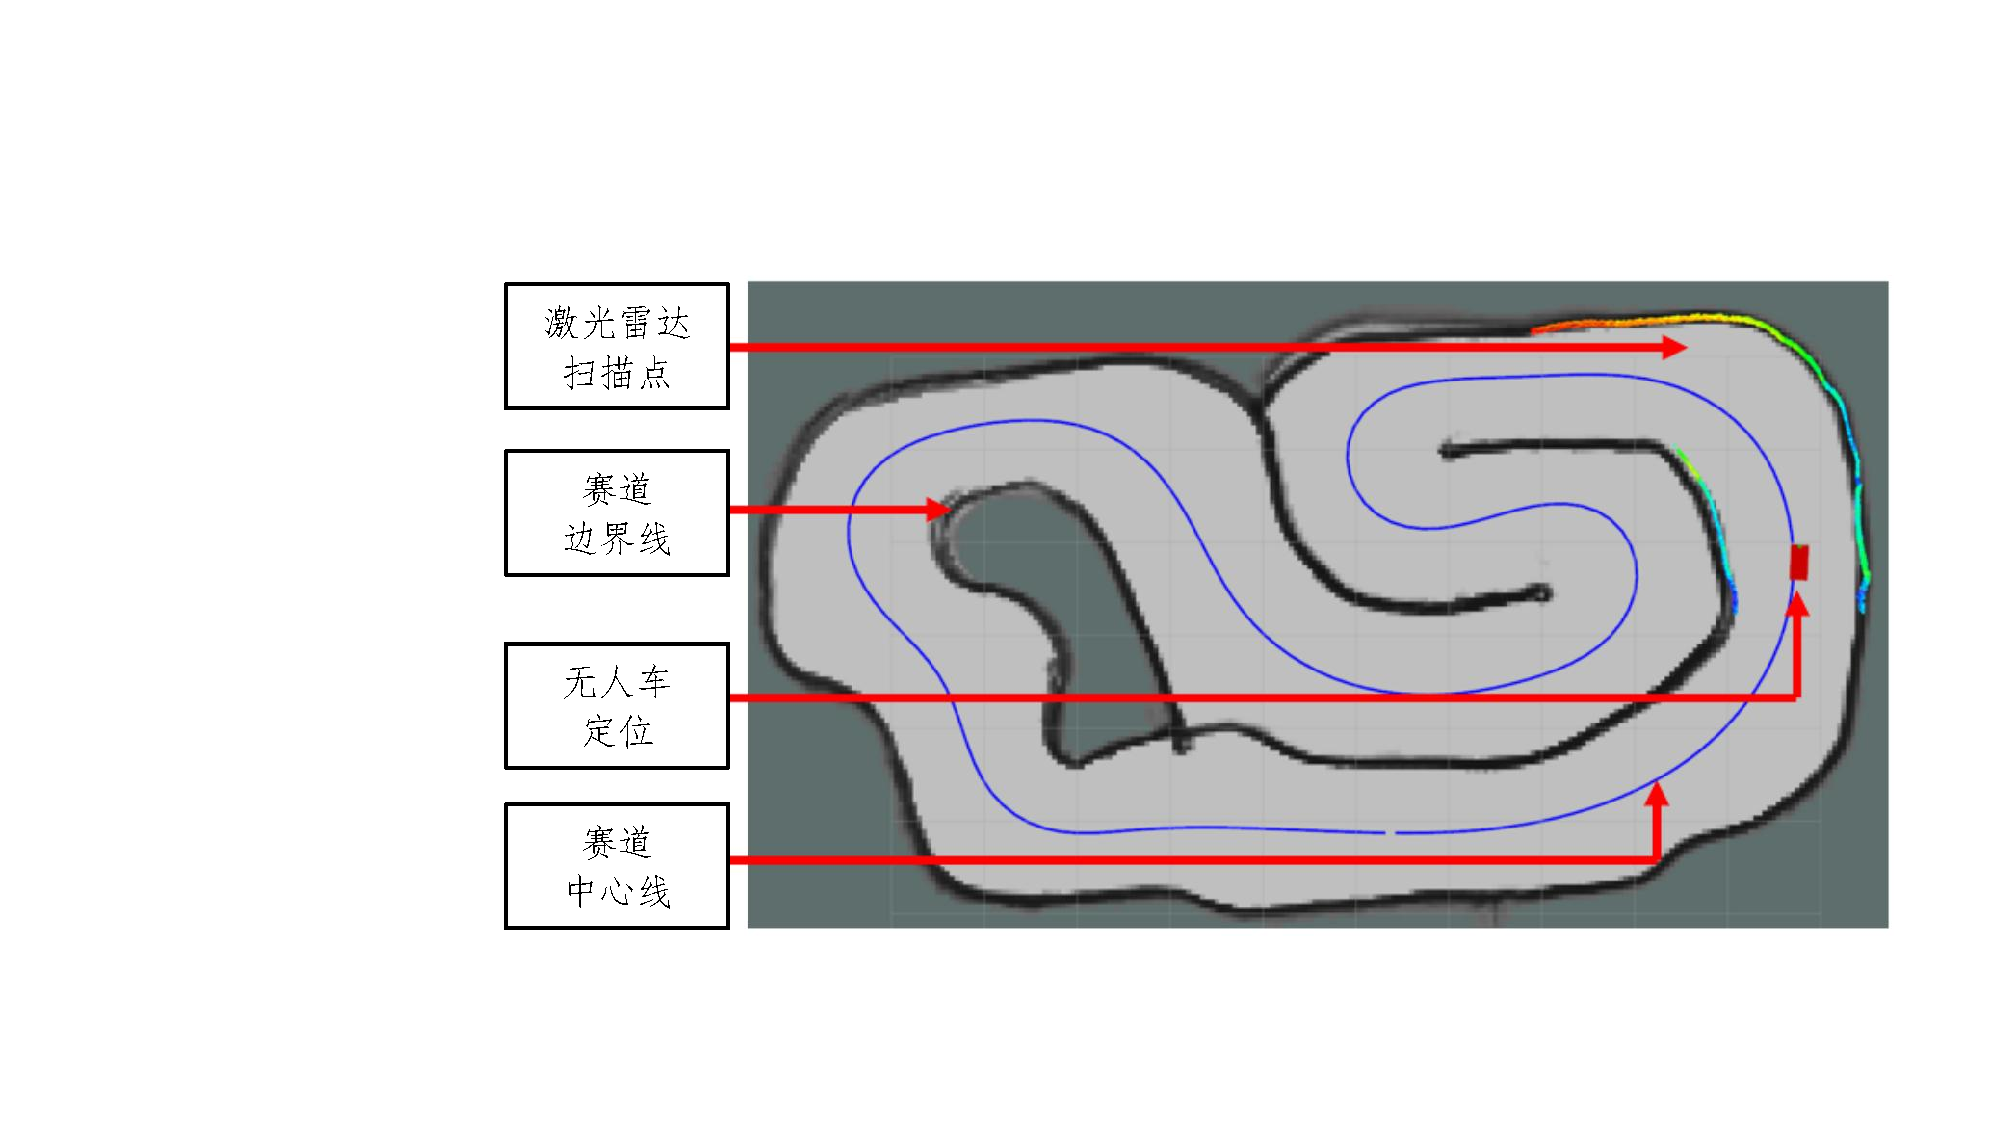
\includegraphics[width=0.7\linewidth]{figure/chapter2/real-map.pdf}
    \caption{实车实验赛道示意图}
    \label{fig:real-map}
\end{figure}
\begin{figure}[H]
    \centering
    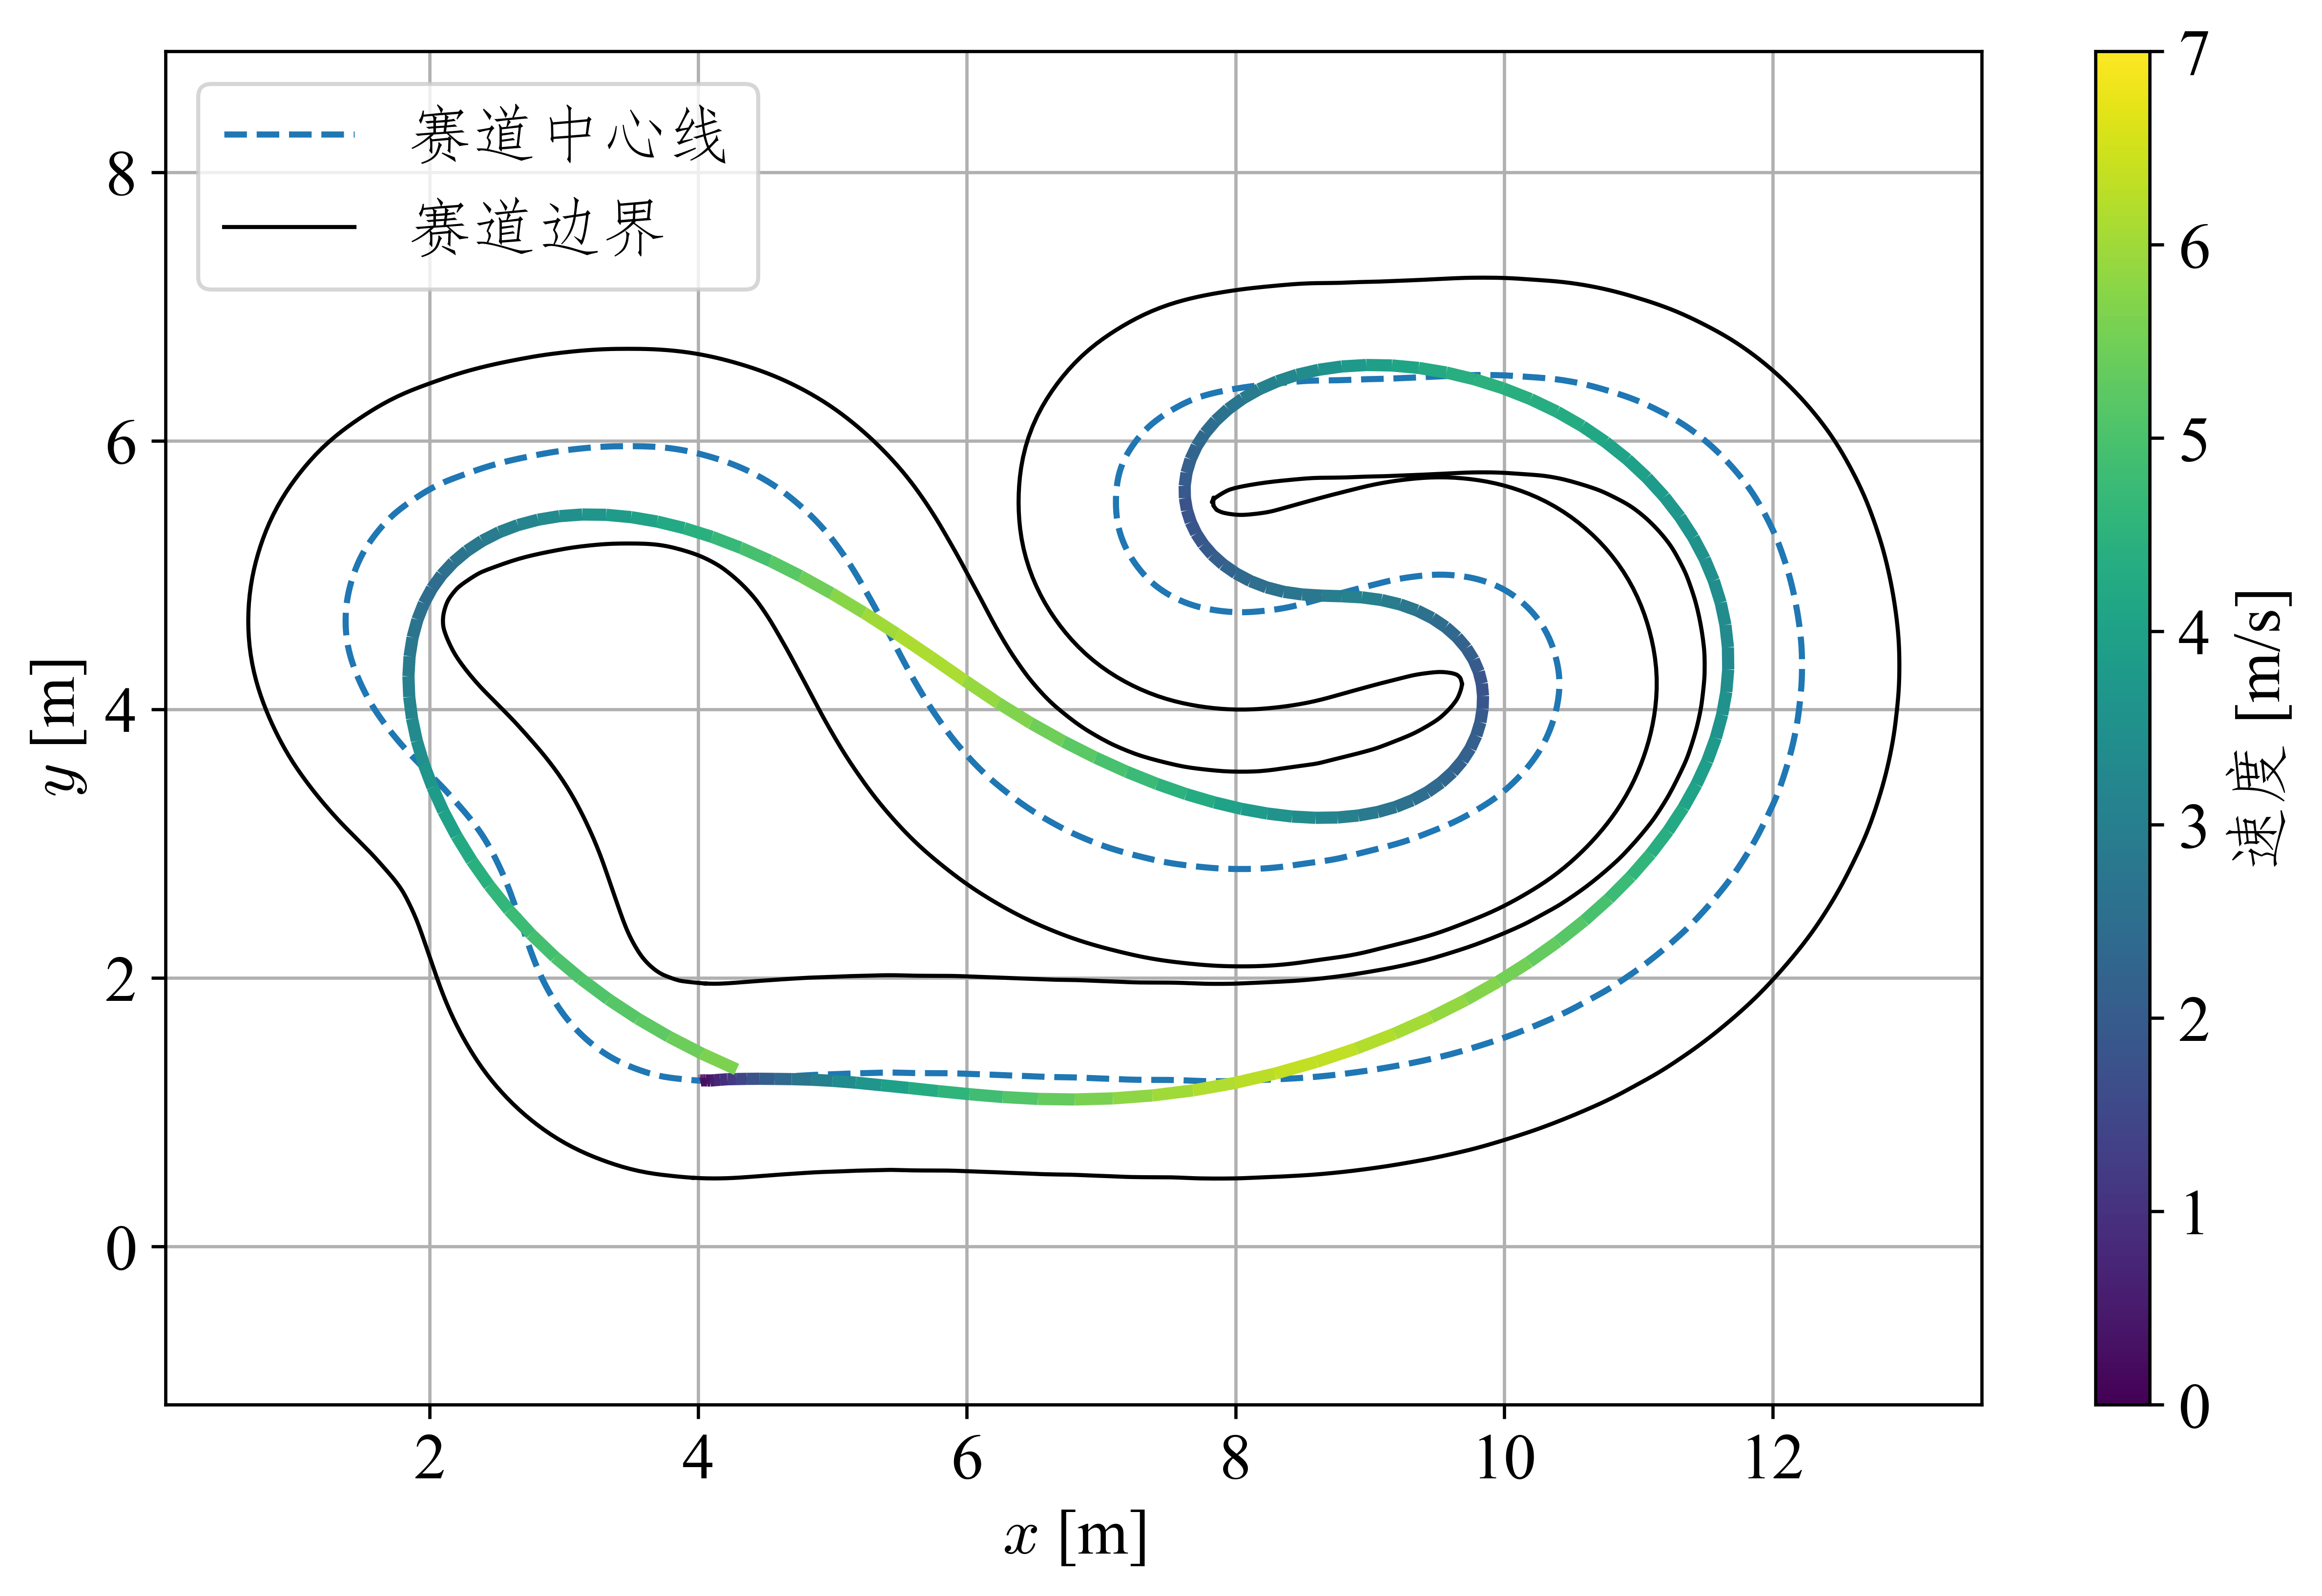
\includegraphics[width=0.7\linewidth]{figure/chapter2/mpcc_cbf_real_trajectory.png}
    \caption{实车实验中的运动轨迹}
    \label{fig:real-trajectory}
\end{figure}
\begin{figure}[H]
    \centering
    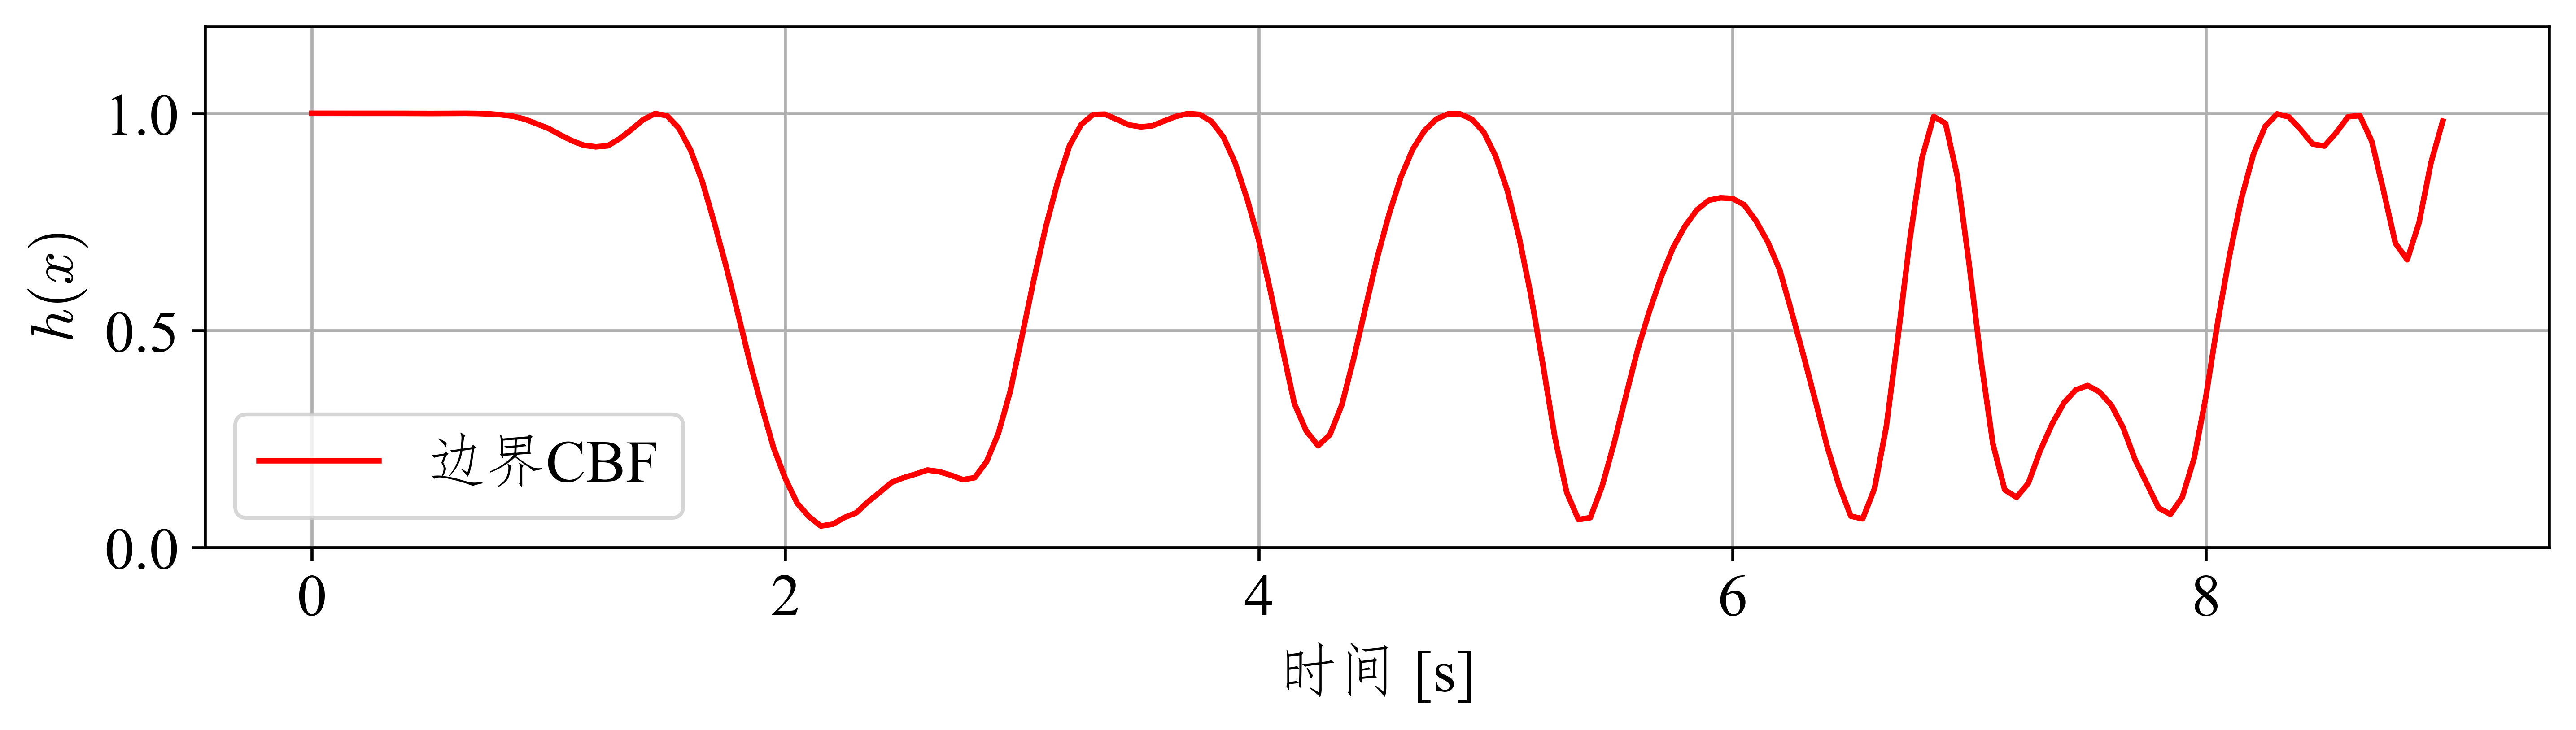
\includegraphics[width=0.75\linewidth]{figure/chapter2/mpcc_cbf_real_cbf.png}
    \caption{实车实验中的控制障碍函数变化曲线}
    \label{fig:real-cbf}
\end{figure}

\begin{figure}[H]
    \centering
    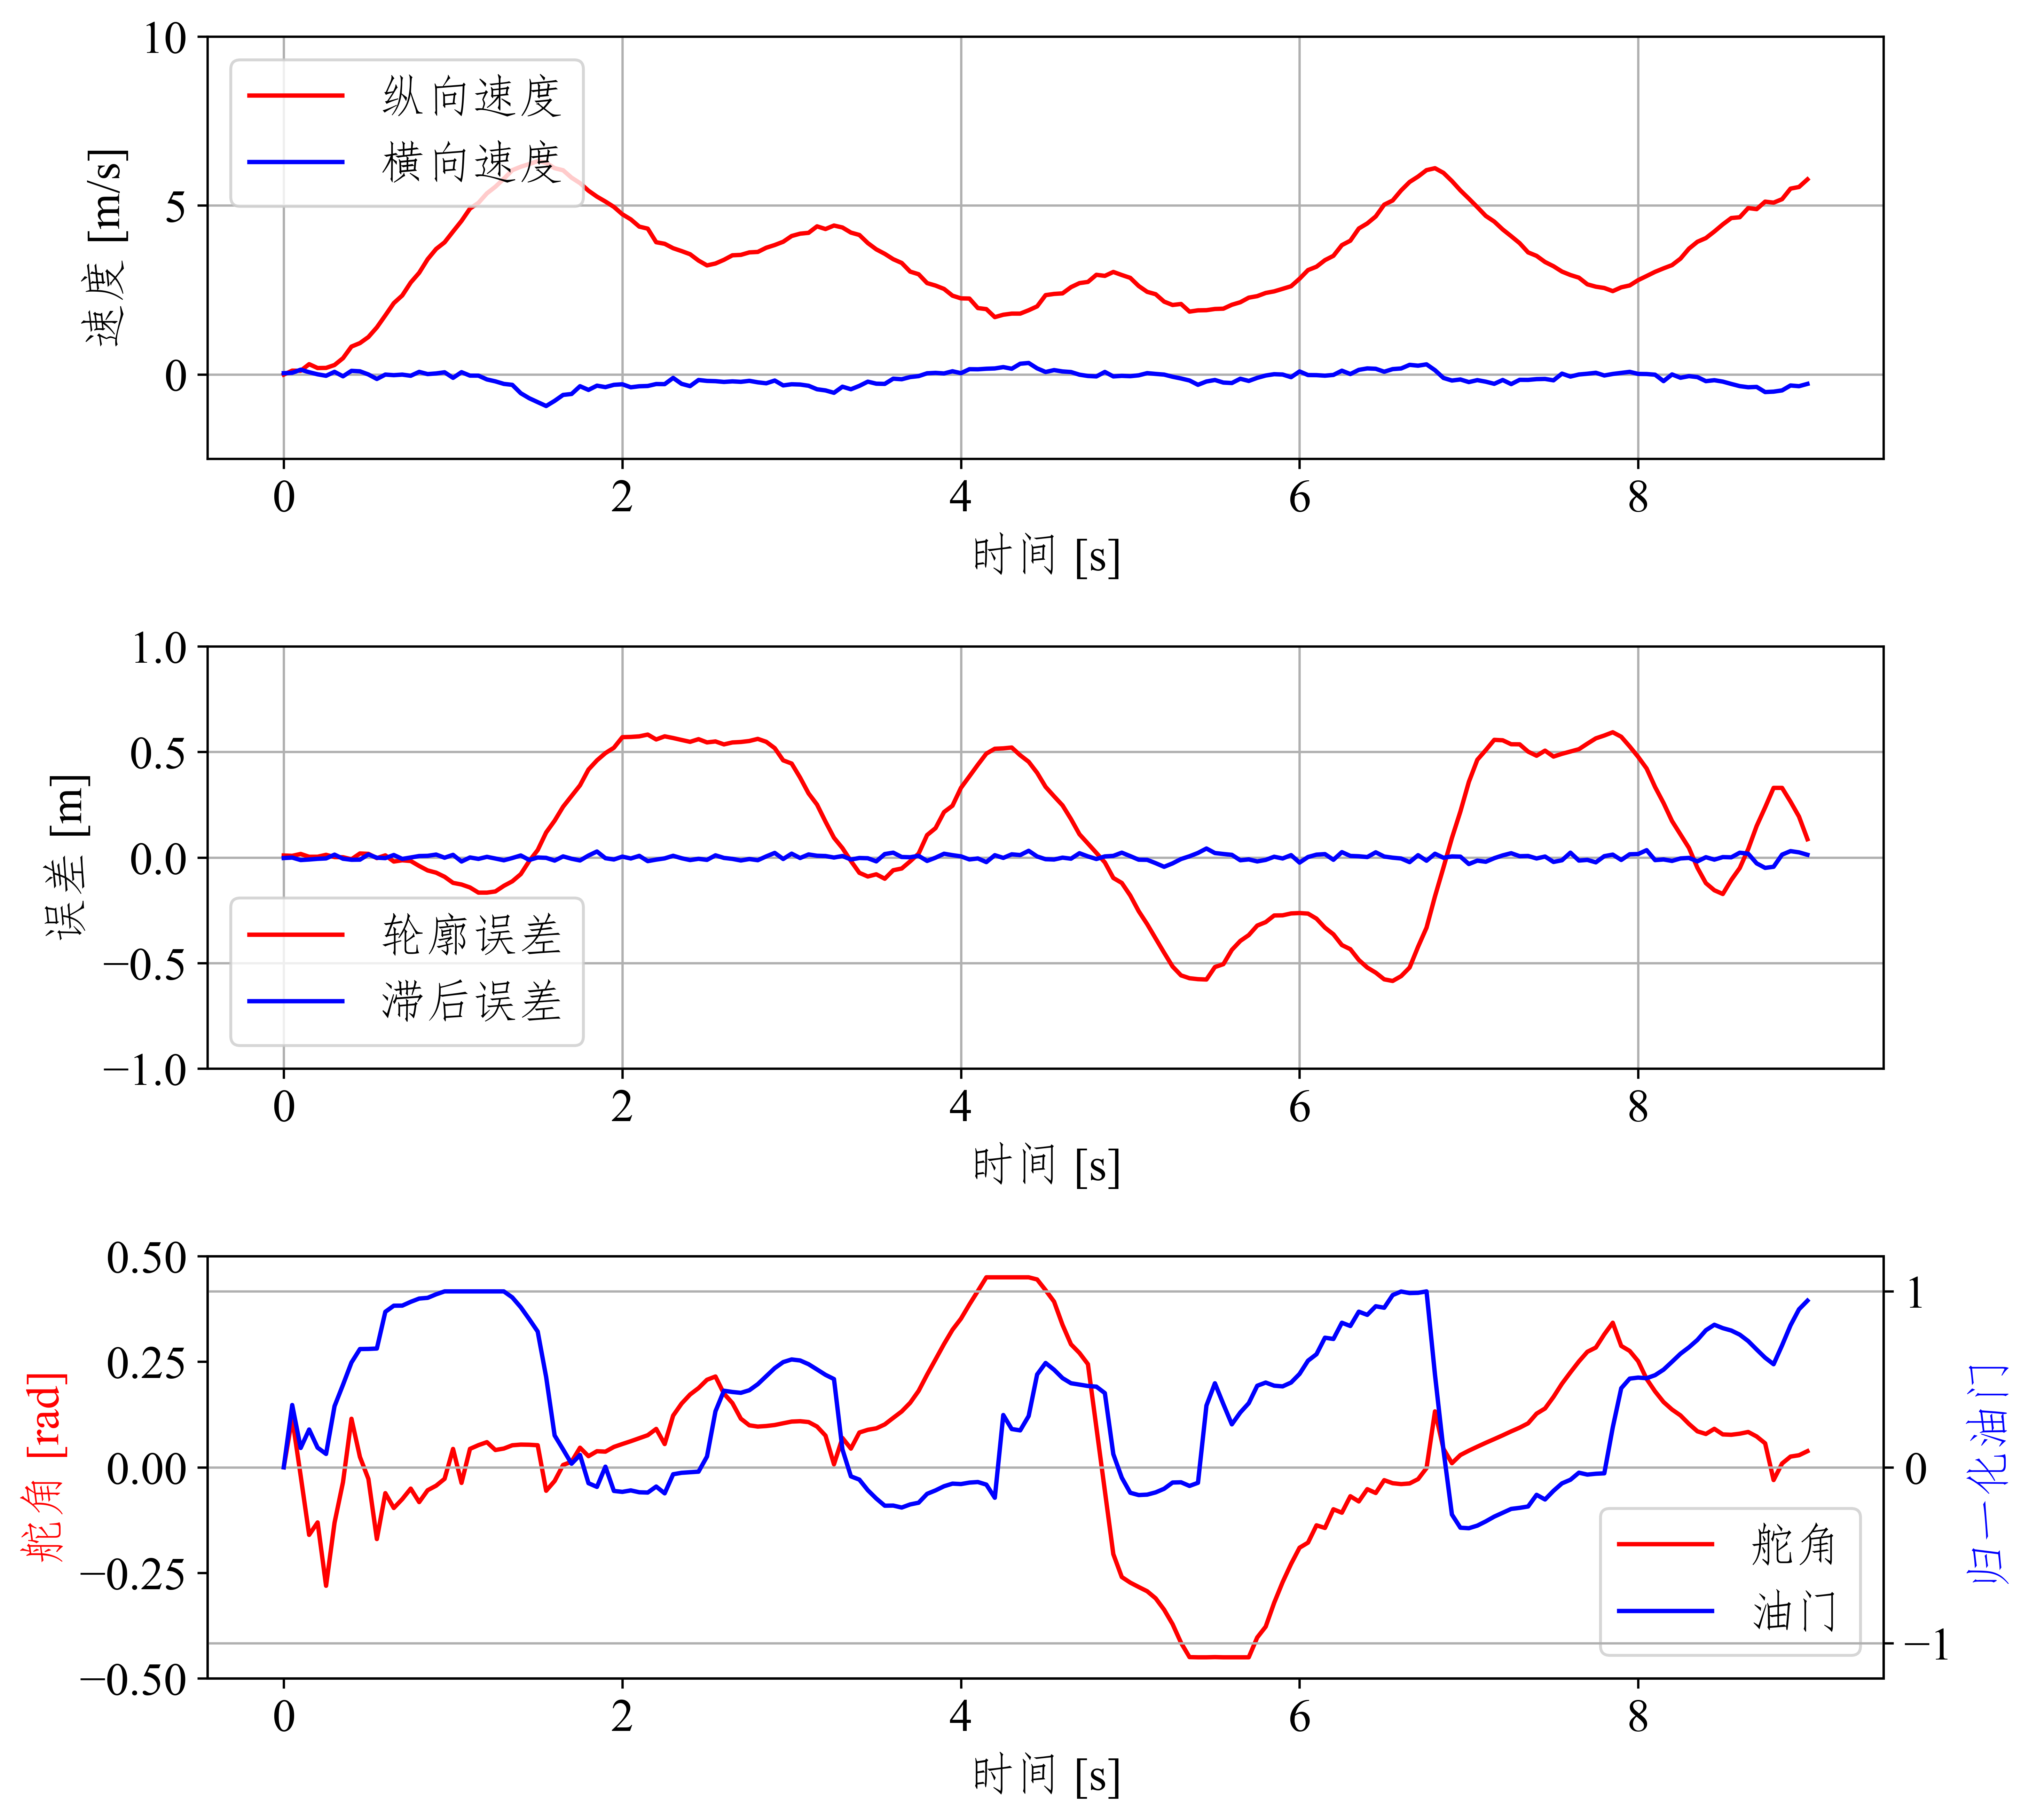
\includegraphics[width=0.8\linewidth]{figure/chapter2/mpcc_cbf_real_control_inputs.png}
    \caption{实车实验中的控制输入变化曲线}
    \label{fig:real-control}
\end{figure}
\begin{table}[H]
    \caption{\label{tab:real-experiment-results}实车实验结果}
    \renewcommand\arraystretch{1.25}
    \begin{tabularx}{\linewidth}{X<{\centering} X<{\centering} X<{\centering}}
    \toprule[2pt]
        参数 & 单位 & 大小 \\ \midrule[1pt]
        单圈时间 & s & $8.97$ \\
        距障碍物最小距离 & m & $0.35$ \\
        平均速度 & m/s & $3.51$ \\
        最大速度 & m/s & $6.35$ \\
        平均计算时间 & ms & $34$ \\ \bottomrule[2pt]
    \end{tabularx}
\end{table}

\newpage
\section{本章小结}
本章提出了一种基于控制障碍函数的模型预测轮廓控制（MPCC-CBF）方法，用于实现安全的竞速运动控制。该方法通过引入一个进度变量来表示赛车在赛道上的路径进度，并通过最小化轮廓误差和滞后误差来优化赛车的竞速性能。同时，控制障碍函数约束确保了赛车在整个竞速过程中始终保持在安全集合内，避免了与赛道边界或其他车辆发生碰撞。通过仿真和实车实验验证了MPCC-CBF控制器在静态和动态环境中的性能，结果表明该方法能够实现高性能的竞速控制，同时具有较强的鲁棒性和安全性。总的来说，MPCC-CBF方法在实现安全竞速控制方面表现优异，能够在保证安全的前提下实现高性能的竞速控制，为自动驾驶赛车领域提供了一种有效的解决方案。